\documentclass[11pt]{article}

%%%\usepackage{lucbr,graphicx,fancyhdr,longtable}
\usepackage{lucidabr,graphicx,fancyhdr,longtable}

\newcommand{\kc}{\textsf{kCARTA}\xspace}
\newcommand{\cm}{\hbox{cm}}

% make a single, doubly indented line 
% (mainly used for driver file examples)
\newcommand{\ttab}{\indent\indent}

\input ASL_defs

\setlength{\textheight}{7.5in}
\setlength{\topmargin}{0.25in}
\setlength{\oddsidemargin}{.375in}
\setlength{\evensidemargin}{.375in}
\setlength{\textwidth}{5.75in}

\newlength{\colwidth}
\setlength{\colwidth}{8cm}
\newlength{\colwidthshort}
\setlength{\colwidthshort}{6cm}

\definecolor{light}{gray}{0.75}

\pagestyle{fancy}

% \date{July 5, 1994} % if you want a hardcoded date

\lhead{\textbf{\textsf{DRAFT}}}
\chead{kCARTA}
\rhead{\textsf{Version 1.11,1.12}}
\lfoot{UMBC}
\cfoot{}
\rfoot{\thepage}

\newcommand{\HRule}{\rule{\linewidth}{1mm}}
\newcommand{\HRulethin}{\rule{\linewidth}{0.5mm}}

\begin{document}
\thispagestyle{empty}
\vspace{2.0in}

\noindent\HRule
\begin{center}
\Huge \textbf{\textsf{kCARTA}}: An Atmospheric Radiative Transfer Algorithm 
using Compressed Lookup Tables
\end{center}
\noindent\HRule

\vspace{0.75in}
\begin{center}
\begin{Large}
Sergio De Souza-Machado, L. Larrabee Strow,\\ Howard Motteler and Scott
Hannon
\end{Large}
\end{center}

\vspace{0.5in}
\begin{center}
Physics Department\\
University of Maryland Baltimore County\\Baltimore, MD 21250 USA\\
\end{center}

\vspace{0.5in}
\begin{center}
Copyright 2002 \\
University of Maryland Baltimore County \\
All Rights Reserved\\
v1.11,1.12  \today\\
\end{center}

\vfill

\noindent\HRulethin
\begin{flushleft}
\begin{tabbing}
Sergio~De~Souza-Machado: \=    sergio@umbc.edu \\
L.~Larrabee~Strow:   \>        strow@umbc.edu\\
\end{tabbing}
\end{flushleft}

%\begin{flushright}
%\includegraphics[width=1.0in]{umseal.eps}
%\end{flushright}

\newpage
\tableofcontents
\listoftables
\listoffigures
\newpage

\begin{center}
{\bf ABSTRACT}
\end{center}
\kc is a radiative transfer code for a non-scattering Earth's
atmosphere.  It can be used to output monochromatic gas optical
depths, layer-to-space transmittances and radiances.  In addition, it can also 
do clear sky radiative transfer computations, or radiative transfer 
computations in the presence of scattering.

In the case of clear sky radiative transfer, \kc can compute and output 
analytic Jacobians with respect to temperature and gas amount.  
 The user can easily change satellite viewing angles
and surface boundary conditions.  As the absorptions coefficients have
been precomputed, the spline interpolations required to compute the
optical depths for arbitrary gas profiles can be done very rapidly, as
can the the spline derivatives needed for the Jacobians.  This makes
\kc very fast.  \kc v1.03+ allows the user to subdivide the lower atmosphere 
layering structure, and then clump together the upper atmosphere layers, 
thereby allowing the program to calculate radiances
for an uplooking instrument more accurately. The namelist files required to 
steer a run are easy to create.  We hope that the ease of use, range of 
features and speed of \kc, make it a useful tool.

In addition to the main \kc source code, some packages need to be picked up
and linked/compiled with the $kcarta$ code. One is $KLAYERS$, which allows an 
user to input a radiosonde or retrieved point profile, and output a layer 
averaged profile that \kc can use. Another is the $RTP$ package, which is a 
AIRS Level II file format. To maintain compatibilty with the AIRS products, 
\kc allows the user to completely or partially interface with the RTP file 
format, which can contain the layer averaged profile and associated 
atmosphere definitions (and convolved radiances). 

We have written and tested a twostream $kSCATTER$ code, which allows fast 
scattering
computations even in the presence of a solar beam. More well known scattering
packages have also been integrated into the code, such as $DISORT$ and 
$RTSPEC$. To produce the Mie scattering parameters required
by both these codes, we have packaged $RTSPEC$, as it contains the code 
necessary ($sscatmie.f$) to produce these parameters for ice and water clouds. 
In addition, for general aerosols, we have interfaced the $OPAC$ database, 
which contains general aerosol properties, with $sscatmie.f$ Along with all 
this, we provide the Fortran and Matlab source code that enables on to read
the output from \kc.

In addition, we have recently begun implementing NonLTE computations into \kc.
As the code essentially performs a line by line spectroscopic computation for
the layers in question, this significantly slows down the code! Currently the
code is optimized for the CO2 4.3 um branch, and closely parallels the GENLN3
code. In addition, we have already included first order linemixing for the R 
branch of the strongest $\Sigma-\Sigma$ band (vib center $\simeq$ 2349 \wn), 
in the 2380 - 2430 \wn temperature sounding region, along with a 
``chi function'' to bring it more into agreement with the full  kCARTA line
mixing.

This document is very much a work in progress.  Some major omissions
include references, significant examples of \kc output, and
comparisons of \kc output to observed spectra.  These omissions will
be rectified in the future.  Please give us your feedback on both the
code and the documentation!  This manual should work for both v1.11 and v1.12.

\newpage
\section{Introduction}

\kc stands for ``kCompressed Atmospheric Radiative Transfer
Algorithm.''  This is an infrared, ``monochromatic'' radiative
transfer algorithm written for a one dimensional non-scattering Earth
atmosphere.  For a downward looking instrument, in a clear sky, 
the surface term and layer emission terms are automatically included in the 
radiative transfer calculation.  In addition, reflected thermal and solar 
terms can also be included :
\begin{equation}
R(\nu) = R_{\hbox{\it surface}}(\nu) + R_{\hbox{\it layer emission}}(\nu) + 
R_{\hbox{\it thermal}}(\nu) + R_{\hbox{\it solar}}(\nu)
\end{equation}
where the terms are the surface, layer emissions, reflected thermal
and solar respectively.  The reflected thermal term is computed
accurately by determining (monochromatically) the layer to ground
cumulative sum of absorption coefficients, and then using an optimum
diffusive angle based on a parameterization of angle as a function of
this cumulative sum.  This makes the inclusion of reflected thermal in
the code quick and accurate.   By differentiating the radiance equation
with respect to a layer gas amount or temperature, the radiance
Jacobian is obtained.  Dropping the surface and reflected thermal terms
enables \kc to compute the radiance measured by an upward looking
instrument as well.  The program can either assume a plane parallel
atmosphere, or include effects on the satellite viewing angle due to
the curvature of the earth.

The absorption coefficients used by the code are computed using a
database of look-up tables.  The look up tables are compressed, using
a Singular Value Decomposition ({\sf SVD}) technique, to produce our
{\sf kCompressed} database.  The point spacing of the current database is
0.0025 \wn, which is an average over five points spaced at 0.0005
\wn.  To compute the absorption coefficients for an arbitrary
profile, the look-up tables are (cubic) spline interpolated in
temperature, and scaled in gas absorber amount.  These splines allow
us to easily compute the analytic temperature derivatives, from
which we can compute temperature Jacobians.

The current database spans 605 \wn to 2805 \wn, broken up into chunks
that are 25 \wn wide.  One hundred pressure layers are used to generate the 
database, from 1100 mb down to 0.005 mb.  These pressure layers are the same 
as those used for the AIRS (Atmospheric InfraRed Sounder) Fast Forward Model, 
for which \kc is the ``Reference Forward Model.''.  The temperatures in the
spectroscopic database are from the U.S. 1962 Standard Profile, as
well as ten temperature offsets (in increments of $\pm$ 10K) on either
side of the Standard Profile.  The current spectroscopic compressed
tables use the {\sf HITRAN98} database for both line-parameters and
cross-sections.  The full and first-order $CO_{2}$ linemixing is from 
refining the modeling undertaken by David Tobin. It should be more accurate 
than that currently in {\sf GENLN2}. in addition, we have used the latest
O2 and N2 continuum models (see Lafferty and J.-M. Hartmann et al in Applied 
Optics 1996, 1997). Other updates to spectroscopy include the ``local'' 
water lineshape as defined by CKD, and the CKDv0, 2.1, 2.3 and 2.4 water 
continuums; in the future we will also add in the $\chi$ function developed 
by D. Tobin. 

\kc is not limited to these pressure levels/layers. $klayers.x$ is a code, 
supplied separately from the \kc distribution, that changes a user supplied 
point profile to a kCARTA layers averaged profile. The default behaviour is 
to use to 
predefined 100 AIRS layers. However, the savvy user can use $klayers.x$ to 
change the pressure levels; these changes then percolate back to \kc.

To maintain compatibility with the AIRS products, for which \kc has been 
developed, the RTP file format and associated libraries need to be linked into
\kc. These files can contain the AIRS profile and the atmosphere definitions 
(such as surface pressure and
temperature, solar reflectance and surface emissivity). \kc allows the user 
to either completely or partially use the information in these files.\\
\textcolor{blue}
{WARNING : If you wish to use RTP, your compiler needs to be able to support 
structures. Currently Absoft, PDF and SGI do, but g77 does not}

In addition, we are adding on more features onto the existing radiative 
transfer algorithm. Currently, it can compute the radiances for either
an upward or downward looking instrument, in a clear atmosphere. The top of 
the atmosphere, and the earth's surface, can be arbitrarily set within the 
pressure level extremes. v1.04 allows the user to compute the upward and 
downward fluxes. Two well known scattering packages, one developed by Frank 
Evans {\em et. al} {\em RTSPEC} and the other by Knut Stamnes et al 
{\em DISORT} has been worked into the kCARTA algorithm. In addition we have 
written our own twostream scattering code {\em TWOSTREAM}. 

We are also working on a perturbative solution to the radiative transfer 
equation, but it has stalled (till Mathematica can solve one of the integrals).
In addition we have used the PCLSAM (Parameterization of Cloud Longwave 
Scattering for use in Atmospheric Models) implementation of Chou, Lee, Tsay 
and Fu's method.

To run any of these scattering  codes, one needs the MIE scattering tables 
generated by F. Evans ``sccatmie'' code. While DISORT is very well tested, it 
is much slower than RTSPEC. RTSPEC runs very fast, almost as fast as 
nonscattering kCARTA, but cannot include the effects of a solar beam. 
$TWOSTREAM$ is a twostream code that runs fast and can include solar beam 
effects. $PCLSAM$ also runs very fast and allows a soalr beam.\\
\textcolor{blue}
{WARNING : If you wish to use DISORT, then your compiler must have the 
autodoubling option, so as to turn REAL variables into DOUBLE PRECISION
variables. If not, then edit file ``scatter\_disort\_code.f'' and change all
occurences of real to double precision}

\textcolor{red}
{The \kc Makefile produces two different executables. 
\begin{itemize}
\item $kcarta.x$ contains all the features of kCARTA (optical depths, clear 
sky radiative transfer, clear sky jacobians and fluxes, $SCATTERING$ 
radiances and fluxes. However, this version uses a $LOT$ of memory
\item $bkcarta.x$ contains only the most basic features of kCARTA 
(optical depths and clear sky radiative transfer). This version uses 
very little memory.
\end{itemize}
}

The speed and features of the code make it an appealing alternative to other
existing ``line by line'' codes such as {\sf GENLN2} and {\sf LBLRTM}.
The accuracy of the database has been extensively compared to {\sf
  GENLN2}.  \kc should contain the latest spectroscopy/lineshape
information.  Furthermore, the code now allows the user to input a set
of externally computed absorption spectra, at various \kc chunks, for one 
gas. The transmittances computed by \kc are smooth and well behaved, which 
will allow people to develop fast-forward models.

\kc is comparatively easy to use. After first picking up and compling the 
$RTP$ and $KLAYERS$ packages, \kc can be compiled, with the right array sizes,
paths to include files and libraries being set in files 
{\sf INCLUDE/kcarta.param, INCLUDE/pre\_defined.param, 
INCLUDE/post\_defined.param  and Makefile}. 
Run time options are set from one driver namelist input file.  We now have 
gone away from the {\sf GENLN2} style driver input files.
\kc is now namelist file driven. However, for users that still wish to use 
the older {\sf GENLN2} style driver input files, we have provided a 
translator code between the old input file and the new namelist (only 
supported upto v1.09).

The driver namelist file contains information such as
start/stop frequency, atmosphere defining information, gas ID's to
be used, and so on.  A layer profile file will also
be read in at this point.  Once the \kc run is complete, supplied
{\sf FORTRAN} or {\sf MATLAB} files can be used to read in the data.

\kc has been written so that it can process one profile at a time. (Note that
while an RTP file can contain more than one profile, \kc can only process
one of the profiles per run). 
Once this profile has been read in, a well written driver input namelist file
can be used to perform many tasks in one run.  For example, it can be
used to compute radiances for many different combinations, such as
with or without solar radiation, with or without background thermal
radiation, different surface temperatures or spectrally varying
emissivities, different start/stop pressures and so on.  For each of
these combinations, clear sky radiance Jacobians can be computed and output. In
the same run, \kc can be used to output layer-to-space transmittances
for various gas combinations, such as all gases combined, all gases
except water, all gases except ozone and so on.  The user can also
choose to output the optical depths of any of the gases read in from
the profile.  Once a \kc run has ended, the user can read in the data
using the supplied readers, or modify the readers to convolve the data
over wanted instrument response functions.

\section{Installing and running \kc}
This is for the user that wants to install and use \kc as quickly as possible. 

\subsection{Distributing \kc}
The distribution is divided into three parts :

\begin{itemize}
\item \textcolor{blue} {Main tarfile $kcartaYYY.tar$} where $YYY$ is the 
version number. This will contain the entire source code distribution (which 
includes the radiative transfer code \kc, and some Matlab and Fortan readers).
There are also some additional data files, and the documentation. This is 
about 80Mb\\
\item \textcolor{blue} {Bugfix tarfile $kcarta\_bugfixYYY.tar$} where $YYY$ 
is the version number.
This will contain the bugfixes, mainly to the radiative transfer code \kc. This
tar file is about 20Mb \\
\item \textcolor{blue} {kCompressed Database} : about 600Mb, supplied on CDs. 
We supply two versions, the big endian or the little endian versions \\
\end{itemize}

\subsection{Installing \kc}
Having obtained the above three, the user can now proceed to install \kc :
\begin{itemize}
\item \textcolor{blue} {Untar $kcartaYYY.tar$} :  this will create a main 
subdirectory, named \kc,
as well as many subdirectories containing the source code, scripts, data files
and so on.
\item \textcolor{blue} {Untar $kcarta\_bugfixYYY.tar$} :  This will overwrite 
the relevant source code files with the latest ones that are deemed bugfree. 
\item \textcolor{blue} {Install datafiles} : Under the KCARTA/DATA 
subdirectory, the user can install (or provide symbolic links to) the 
$CompDataBase$ and $WaterDataBase$ files provided in the diskettes 
containing the kCompressed Database
\item \textcolor{blue} {Create a WORK directory} : Create directory WORK
under the KCARTA directory
\end{itemize}

\subsection{Compiling the packages}
Now the source code compilation can begin. There are three main sets of code
that have to be compiled. We will decribe the compilation assuming the user 
is going to use the 100 AIRS pressure layers/levels, instead of changing the 
pressure levels. Before compiling each of the three packages described below, 
the user should edit the relevant Makefile so that his/her preferred F77 
compiler will be called. We have tested the package mainly on Unix style 
SGI and Absoft machines. The flags for these compilers are
\begin{verbatim}
# SGI Fortran
# ------------
# SGI compiler options
# -u  : turn off implicit typing of variables
# -g  : generate debugging information (turns off optimization)
# -C  : do run time subscript range checking
# -w0 : inform about unused variables
# -O3 : heavy optimization
# -64 : 64-bit objects (libraries must match)
\end{verbatim}
\begin{verbatim}
# Linux with Absoft Fortran
# --------------------------
# Absoft compiler options
# -f    fold all names to lower case
# -N109 fold all names to upper case
# -W    wide source file
# -w    suppress warning messages (absoft is more fussy than SGI or g77)
# -A    alignment warnings
# -C    check array bounds
# -O    some optimizations
# -N3   add record info to unformatted files
# -s    static allocation
# -N2   force intrinsic double functions
# -N113 force double precision
# -N114 force untyped variables as warnings
\end{verbatim}

If Absoft is used, since it is quite fussy, there might be a few warning 
messages produced during the compilations.

\begin{itemize}
\item \textcolor{blue} {SRC symbolic link} :  At the main KCARTA 
subdirectory, make sure that the ``SRC'' symbolic link points to ``SRCv1.11''
\item \textcolor{blue} {BLAS library} : If your computer has a BLAS library, 
you can skip this part. Else go to the KCARTA/LIB/blas.ref subdirectory, and 
type ``make'' (at present the Makefile assumes a LINUX Absoft F77 compiler.
\item \textcolor{blue} {klayers} Go to KLAYERS/Src. Edit the 
``Makefile'' so that the compiler options are those that exist on your 
machine. Type ``make''. This should produce a file \textcolor{red}{klayers.x}.
\item \textcolor{blue} {kcarta} The \kc Makefile can make one or all of 
three different executables. For the basic distribution that will satisfy 
most people, only \textcolor{red} {bkcarta.x} is produced.
Go to KCARTA/SRC. Edit the ``Makefile'' so that the 
compiler options are those that exist on your machine. Edit the little endian 
vs big endian part of the ``kcarta.param'' file, so that the correct paths
are set for the data files (ensure that the kCompPath,kCO2Path,
kCOusin\_CO2Path and kWaterPath 
strings point correctly to the database files, while kCKDPath,kSolarPath and 
kXsecFile point to the correct be vs le files). Type ``make''. If everything 
compiles ok, file \textcolor{red}{bkcarta.x} will appear in the 
KCARTA/BIN directory
\begin{itemize}
\item $kcarta.x$ contains all the features of kCARTA (optical depths, clear 
sky radiative transfer, clear sky jacobians and fluxes, $SCATTERING$ radiances
and fluxes. However, this version can use a $LOT$ of 
memory
\textcolor{red}
{\item $bkcarta.x$ contains only the most basic features of kCARTA 
(optical depths and clear sky radiative transfer). This version uses 
very little memory.}
\end{itemize}
\item \textcolor{blue} {readers with fseek} Go to 
KCARTA/UTILITY. If your compiler supports the  ``fseek'' subroutine, type 
``make'' at the prompt. If everything compiles ok, 
file \textcolor{red}{readkcBasic.x} will appear in the KCARTA/BIN directory.
Note that Absoft F77 can act funny with the fseeks, so it might be better to 
use the g77 compiler here. If this is the case then edit files 
$readkcBasic.f$ and $readbinary.f$, replacing 
\textcolor{red}{iDummy = fseek(,...)} with
\textcolor{red}{CALL fseek(,...)} with
as well as removing FSEEK from the local variables declarations
\item \textcolor{blue} {readers without fseek} Go to 
KCARTA/UTILITY/READwoFSEEK. If your compiler does not support the 
``fseek'' subroutine, type ``make'' at the prompt. If everything compiles ok, 
file \textcolor{red}{readkcBasic.x} will appear in the KCARTA/BIN directory.
\end{itemize}

\subsection{Checking the \kc installation}

If all this has been accomplished successfully, the user is now ready to try 
running \kc. Change to the KCARTA/SCRIPTs directory and type \\
\begin{center}
\textcolor{red} {basic.sc sondeprofile outputfile}
\end{center}

Here $sondeprofile$ is the name of the input radiosonde profile. 
This input profile will be processed through $klayers.x$, producing a layer
averaged profile $kcarta.op.rtp$ in the KCARTA/WORK subdirectory. After that,
$bkcarta.x$ runs, reading in namelist file $basic.nml$ (see below) and profile
$kcarta.op.rtp$. The output of $bkcarta.x$ is stored in a large binary file,
$outputfile$.  This binary output file consists of a header, which
contains information that determine the overall size of the file. After this 
comes the actual binary data. Since \kc works in chunks of 10000 points, 
all the outputs for the first 10000 points are written out, followed by the
outputs for the next 10000 points and so on. 

As an example to use this script, type 
\begin{center}
basic.sc BASIC/USStandardProf\_NEW ../WORK/out.dat
\end{center}

To read the contents of this file, one can use either the $readkcBasic.x$ 
(Fortran) or the $readkcBasic.m$ (Matlab) readers. These readers go ahead 
and ``unchunk'' the data, as shown in the figure below. 

As would be evident from reading the more extensive documentation, \kc works 
in chunks of 10000 points. For example, suppose the user wants 100 mixed 
paths to be output from 605 to 705 $cm^{-1}$ . These mixed paths, 1-100, in 
region 605-630 $cm^{-1}$ are processed and output first. These are followed 
by the 100 mixeed paths in region 630-655 $cm^{-1}$, and so on.

However, most users would want the data in the following format. Mixed path 
1, from 605 to 705 $cm^{-1}$, followed by mixed path 2 in this complete 
wavenumber interval, and so on, uptil mixed path 100. As seen from the 
Figure ~\ref{translatingfiles}, the  $readkcBasic.x$ (Fortran) and the 
$readkcBasic.m$ (Matlab) readers ``reshape'' the matrices that \kc outputs, 
to be in this more convenient format.

$basic.sc$ calls $readkcBasic.x$ and translates file $../WORK/out.dat$ 
(on the left) to a very simple binary file $../WORK/outfile.bin$ 
(on the right of the figure). The only possible problem is that to make this
Fortan reader work fast, we have used the nonstandard ``fseek'' option. 
This seems to work fine with SGI Fortran and g77 on Linux, but causes grief
if used with Absoft.

\begin{figure}
\includegraphics[width=5.5in]{FIG/example_109.eps}
\caption{Translating the output file.}
\label{translatingfiles}
\end{figure}

\subsection{Checking the \kc installation}

The format of the final binary file (shown on the right in the figure above)
is very simple :
\begin{itemize}
\item iSetMin : 1 integer, stating starting index (= 1)
\item iSetMax : 1 integer, stating ending index (= 10000 x iNumChunks)
\item iTotal  : 1 integer, telling how many outputs per chunk
\item Freqs   : 10000 x iNumChunks, giving the kCARTA wavenumbers (reals)
\item Data    : (10000 x iNumChunks) x iTotal, giving the data (reals)
\end{itemize}
If  $ 10000 x iNumChunks = iX$ then the $Freqs$ are output in one Fortran
data block. Similarly the $Data$ is in iTotal rows, each of which contain 
$iX$  elements. So the whole file can be read using a simple program such as

\begin{verbatim}

integer iOUN,iSetMin,iSetMax,iTotal,iX,iR,iFr,iRows,iChunks
real raWaves(10000*iChunks),raaData(iRows,10000*iChunks)

read(IOUN) iSetMin
read(IOUN) iSetMax
read(IOUN) iTotal
iX = iSetMax - iSetMin + 1
read(IOUN) (raWaves(iFr),iFr = 1,iX)
DO iR = 1,iTotal 
  read(IOUN) (raaData(iR,iFr),iFr = 1,iX) 
  END DO 
\end{verbatim}
Typically, for a 100 layer atmosphere, iTotal is about 500 (five sets of 
mixed paths), while iX is an integer multiple of 10000 points (eg for a 
typical AIRS channel, this would probably span one or two kCARTA chunks, which
would be about 10000 or 20000 points).

\section{A Walk Through a \kc Session}

\kc is packaged so that it is easy to set up and start using.  In
order to run the code, the user has to unzip and untar the
distribution; this automatically sets up the correct directory
structure.  The file {\sf README.1ST} describes the steps necessary
to compile the source code for \kc and for the various {\sf UTILITY}
files we include with the package.  After this is done, a script
file can be run, so that the user can check to see if his/her setup
obtains the same test results as we supply in the {\sf COMPARISON}
subdirectory.

At present, the 600 Mb kCompressed Database is distributed on tape.
In the future, we plan to distribute the \kc package on CD in two
parts; the {\sf SVD} compressed database and a zipped tar file of
the source code.  The user has to put the database into the {\sf
DATA/CompDataBase}, {\sf DATA/WaterDataBase} subdirectories.  At
this point, the user can ensure that he/she has the correct summary
of the files in the database.  This is achieved by a run of program
{\sf compdatabase.x}, which produces a parameter file {\sf
comp97.param} summarizing the database.  {\sf compdatabase.f} is one
of the utility programs supplied along with the \kc package, and is
found in the {\sf UTILITY} subdirectory.  Typing ``make'' in that
subdirectory will compile the source files and place them in the
binary subdirectory {\sf BIN}.

The user can now go to the source subdirectory {\sf SRC}, and use
the {\sf makefile} there to compile the main source code.  Assuming
the {\sf BLAS} routines (if needed) have also been
successfully compiled and can be linked in, the code is now ready to
be run.  All it requires are driver namelist input files.

We now give an overview and example of the driver namelist file; a more
detailed view will be given in subsequent sections.  The example has
purposely been written so that \kc does a fairly comprehensive
demonstration of its abilities---radiances for downlooking and
uplooking instruments, solar and thermal background radiation
alternately turned on or off, compute jacobians and so on.  (Of
course, this means the output file from this run will be quite
large!).  All the lines that begin with {\tt !} are comment lines,
and will explain to the reader what the different inputs are.  A
brief description of the purpose/effects of the file is as follows.
The first section asks \kc to use water continuum version CKDv2.1,
as well as to output all spectra as layer-to-space transmittances.
The frequency region is from 2705~to~2780~ $\cm^{-1}$.  We have
chosen to explicitly specify which gasIDs are to be used from the
compressed database, while the program is asked to include the
required gases automatically from the crosssection database.  \kc is
asked to read in supplied regression profile \#1, which happens to
be the {\sf AFGL} tropical (hot/humid) profile.

Note that in this example, we have turned on the water continuum (kCKD=21),
and so we explicitly ask \kc to include gases 101,102 which are the self and 
foreign water continuums.

In this example the gas absorption coefficients will be weighted and
combined in two  different ways, one where all gases are equally
weighted by unity, the second where water (and self and foreign continuums) 
and ozone weights differ slightly from unity. We can use these weights to 
define three separate atmospheres, for the program to do radiative transfer
calculations. The first two atmospheres are defined
so that the high-in-the-sky instrument is downward looking (in
addition to the surface and layer emission terms, one atmosphere has
both solar and background thermal turned on, while the other only
has background thermal turned on).  The third atmosphere is for an
upward looking instrument that is close to the ground, with the sun
filling the field of view.  Jacobians will be computed and output
for all the three atmospheres.

We have now added on scattering routines and the ability to import line by 
line spectra computed by an external code. In the example below, we use 
externally generated spectra for some CO2 regions and for some N2O regions. 
In addition, a two layer cloud is also specified.

The output section asks \kc to output radiances for all three
atmospheres (at different pressure levels), output all layer-to-space
transmittances, and output gas spectra for GasID=2.  

Note that \kc will not really accept this namelist file, as it asks for
Jacobians to be computed, in addition to scattering computations and 
importing external LBL spectra. In addition, it will complain as the output
section asks for multi level radiance outputs. If you turn off the Jacobians, 
as ask for radiances to be output only at one level for each atmosphere, 
the namelist driver file will be successfully parsed in.

Here is the sample namelist river file (which we name example.nml) :

\begin{scriptsize}
%\begin{small}
\begin{verbatim}

 $nm_params
 namecomment    =  '******* PARAMS section *******'
 !set this to output layer to space transmittances
 kLayer2Sp = 2
 !set this to v2.4
 kCKD      = 24
 !set kRTP = 0 so we read only the profile from the RTP file
 kRTP = 0
 $end

 $nm_frqncy
 namecomment    =  '******* FRQNCY section *******'
 rf1            = 905.000
 rf2            = 1005.000
 $end
 $nm_molgas

 namecomment    =  '******* MOLGAS section *******'
 !use  water, carbon dioxide, ozone, nitrous oxide,  methane, HCl and H2CO 
 ! as well as the self and foreign continuums 
 iNGas     =            9,
 iaGasesNL = 1, 2, 3, 4, 6, 15, 20, 101, 102
 $end

 $nm_xscgas
 namecomment    =  '******* XSCGAS section *******'
 !use all minor cross section gases
 iNxsec =            -1
 $end

 $nm_prfile
 namecomment    =  '******* PRFILE section *******'
 caPfname       =  'testprof0.op.rtp'
 $end

 $nm_weight
 namecomment    =  '******* WEIGHT section *******'
 !define 2 sets of mixed path sets
 iNpmix =             3
 caaMixFileLines        = 
 !first set has all gases weighted by 1.0
                          '1   -1    1.0    -1',
 !second set has all gases weighted by 1.0, except water and CO2
                          '2   -1    1.0    4',
                             '1 1.12 3 1.03 101 1.12 102 1.12',
 $end

 $nm_radnce
 namecomment    =  '******* RADNCE section *******'
 !define 3 atmospheres
 iNatm          =  3

 !use WEIGHT set number 1 (from above, this is all gases weighted by 1.0). 
 !The pressure endpts are from 971 to 0.0 mb (so radiation is travelling 
 !upwards, to the down looking instr at 0.0 mb)
 !space temp=2.96K, surface temp=308.34k, 
 !satel view angle=20 degrees, do not include geometry effects in angle
 iaMPSetForRad(1)   =  1
 raPressStart(1)    =  971.7370000
 raPressStop(1)     =  0.0
 raTSpace(1)        =   2.960000
 raTSurf(1)         =  308.3
 raSatAngle(1)      =  0.0000000E+00
 raSatHeight(1)     =   1.00
 ! turn off solar (-1), solar angle=0.0, use surface emiss(-1.0),
 ! turn on thermal diff approx, (0), thermal angle=53 degrees (-1),
 !include thermal background if Jacobians are computed (1)
 iakSolar(1)        =  -1
 rakSolarAngle(1)   =  0.0000000E+00
 cakSolarRefl(1)    =  'NONESPECIFIED'
 iakThermal(1)      =   0
 rakThermalAngle(1) =  -1.000000
 iakThermalJacob(1) =   1
 !use the following data file for spectral dependent surface emissivities
 caEmissivity(1)    =   '../DATA/General/emissivity.dat'
 raSetEmissivity(1) =  -1.000000

 !use WEIGHT set number 2 (from above, this is all gases weighted by 1.0, 
 !except water and ozone). The pressure endpts are from 1200.0
 !to 10.0 mb (so radiation is travelling upwards, to the down looking instr)
 !space temp=2.96K, surface temp=303.34k, 
 !satel view angle=0 degrees, do not include geometry effects in angle 
 iaMPSetForRad(2)   =  2
 raPressStart(2)    =  1200.0000
 raPressStop(2)     =  10.0
 raTSpace(2)        =   2.960000
 raTSurf(2)         =  303.34
 raSatAngle(2)      =  0.0000000E+00
 raSatHeight(2)     =   -1.000000
 !turn on solar (1), solar angle=0.0, use surface emiss (-1.0),
 ! turn on thermal accurate quadrature(1), thermal angle=53 degrees (-1 says 
 ! use this default), include thermal background if Jacobians are computed (1)
 iakSolar(2)        =  1
 rakSolarAngle(2)   =  0.0000000E+00
 cakSolarRefl(2)    =  '../DATA/General/sunrefl.dat'
 iakThermal(2)      =   1
 rakThermalAngle(2) =  -1.000000
 iakThermalJacob(2) =   1
 !use the following data file for spectral dependent surface emissivities
 caEmissivity(2)    =   '../DATA/General/emissivity.dat'
 raSetEmissivity(2) =  -1.000000

 !use WEIGHT set number 1 (from above, this is 2 -1 1.0 -1, which means all 
 ! gases weighted by 1.0). The pressure endpts are from 0.0
 ! to 985.0 mb (so radiation is travelling downwards, to the up looking instr)
 !space temp=5600k (iakSolar = +1, sun fills FOV), dummy surface temp=303.34k, 
 !satel view angle=10 degrees,  include geometry effects in angle
 iaMPSetForRad(3)   =  1
 raPressStart(3)    =  0.0000
 raPressStop(3)     =  985.0
 raTSpace(3)        =  2.96.0000
 raTSurf(3)         =  303.34
 raSatAngle(3)      =  10.0000000E+00
 raSatHeight(3)     =   705.0
 ! as we have upward looking instrument, just give six dummy values
 iakSolar(3)        =  1
 rakSolarAngle(3)   =  0.0000000E+00
 cakSolarRefl(3)    =  'dummysun'
 iakThermal(3)      =   0
 rakThermalAngle(3) =  -1.000000
 iakThermalJacob(3) =   1
 ! as we have upward looking instrument, just give a dummy emissivity
 caEmissivity(3)    =   'dummy'
 raSetEmissivity(3) =  0.9
 $end

 $nm_jacobn
 namecomment    =  '******* JACOBN section *******'
 !NOTE : THIS TELLS YOU HOW TO ENTER JACOBIAN SECTION; SINCE "SCATTER" AND
 !"SPECTRA" BELOW ARE ON, THE CODE WILL NOT ALLOW YOU TO COMPUTE JACOBIANS!

 !if you want to turn off NEWGASES , simply put iNumNewGases = -1 BELOW
 !if you want to turn off SCATTERING, simply put kScatter = -1 BELOW

 !compute two gas jacobians
 iJacob =             2
 !the gas IDs are 2,6  (co2 and n20)
 iaJacob  = 2,6
 $end

 $nm_spectr
 namecomment    =  '******* SPECTRA section ******'
 !if you want to turn this off, simply put iNumNewGases = -1

 !use externally generated LBL spectra for two gases
 iNumNewGases   =             2

 !the girst gas has ID = 2 (CO2), with 6 new chunks of data
 iaNewGasID(1)  =             2
 iaNewData(1)   =             6
   iaaNewChunks(1,1)    =           2305
   iaaNewChunks(1,2)    =           2330
   iaaNewChunks(1,3)    =           2355
   iaaNewChunks(1,4)    =           2380
   iaaNewChunks(1,5)    =           2405
   iaaNewChunks(1,6)    =           2430
   caaaNewChunks(1,1)    =   '../DATANEW/co2_2305'
   caaaNewChunks(1,2)    =   '../DATANEW/co2_2330'
   caaaNewChunks(1,3)    =   '../DATANEW/co2_2355'
   caaaNewChunks(1,4)    =   '../DATANEW/co2_2380'
   caaaNewChunks(1,5)    =   '../DATANEW/co2_2405'
   caaaNewChunks(1,6)    =   '../DATANEW/co2_2430'

 !the girst gas has ID = 4 (N20), with 2 new chunks of data
 iaNewGasID(2)  =             6
 iaNewData(2)   =             1
   iaaNewChunks(2,1)    =           2255
   iaaNewChunks(2,1)    =           2280
   caaaNewChunks(2,1)     =   '../DATANEW/nitrousoxide2255'
   caaaNewChunks(2,1)     =   '../DATANEW/nitrousoxide2280'
 $end

 $nm_nonlte 
 namecomment    =  '******* NONLTE section ******' 
 !!!turn on nonlte
 iNumNLTEGases    =             +1 

 !!use the slow accurate LBL model
 iNLTE_SlowORFast =             +1

 iDoUpperAtmNLTE    = +1
 caaUpperMixRatio = '/home/sergio/KCARTADATA/General/NLTE/atm_md.ip'

 iAllLayersLTE      = -1
 iUseWeakBackGnd    = +1
 iSetBloat          = +1

 iaNLTEGasID(1)      =        2
 raNLTEstrength(1)   =        1.000
 raNLTEstart(1)      =        30.0
 iaNLTEChunks(1)       =        10

 !comment out this so kCARTA finds optimum profile!!!!!
 !!!caaNLTETemp(1)     = 
 !!!  '../SRC/NONLTE2/sergio/VT_48PROFILES/sergio_merge/vt5_s0.prf'
 caaStrongLines(1) = 
     '/carrot/s1/sergio/AIRSCO2/CO2_BANDS_PARAM/co2_4um_bands.txt'

 iaaNLTEChunks(1,1)  =         2230
 iaaNLTEChunks(1,2)  =         2255
 iaaNLTEChunks(1,3)  =         2280
 iaaNLTEChunks(1,4)  =         2305
 iaaNLTEChunks(1,5)  =         2330
 iaaNLTEChunks(1,6)  =         2355
 iaaNLTEChunks(1,7)  =         2380
 iaaNLTEChunks(1,8)  =         2405
 iaaNLTEChunks(1,9)  =         2430
 iaaNLTEChunks(1,10) =         2455

 iaNLTEBands(1)     = 19
 !!! uses strongest  sigma-sigma, pi-pi, delta-delta 
 !!! 2350 .. 2354 = sigma-sigma 
 !!! 2320 .. 2322 = pi-pi 
 !!! 2310 .. 2312 = delta-delta 
 !!!                 GASID   GASIso  iLSGQ     iUSGQ   run7lblID 
 caaaNLTEBands(1,1) ='2        1       1         9        2350' 
 caaaNLTEBands(1,2) ='2        2       1         9        2351' 
 caaaNLTEBands(1,3) ='2        3       1         9        2352' 
 caaaNLTEBands(1,4) ='2        4       1         9        2355' 
 caaaNLTEBands(1,5) ='2        1       2         16       2320' 
 caaaNLTEBands(1,6) ='2        2       2         16       2321' 
 caaaNLTEBands(1,7) ='2        1       4         24       2310' 
 caaaNLTEBands(1,8) ='2        2       4         24       2311' 
 caaaNLTEBands(1,9) ='2        1       3         23       2353'  
 caaaNLTEBands(1,10)='2        1       5         25       2354'  
 !!!these are the ones Manuel suggested adding on; some isotopes of above
 caaaNLTEBands(1,11)='2        2       3         23       2253'  
 caaaNLTEBands(1,12)='2        2       5         25       2254'  
 !!!these are the others Manuel suggested adding on
 caaaNLTEBands(1,13)='2        1       2         15       2110'  
 caaaNLTEBands(1,14)='2        1       3         25       2120'  
 caaaNLTEBands(1,15)='2        1       5         23       2140'  
 caaaNLTEBands(1,16)='2        1       6         36       2160'  
 caaaNLTEBands(1,17)='2        1       7         37       2170'  
 caaaNLTEBands(1,18)='2        1       8         38       2180'  
 caaaNLTEBands(1,19)='2        3       2         16       2322'
 !!!these one never seems to exist in the NLTE profiles
 caaaNLTEBands(1,20)='2        1       3         22       2150'  
 caaaNLTEBands(1,21)='2        1       4         22       2130'  
 $end

 $nm_scattr
 namecomment    =  '******* SCATTR section *******'
 !if you want to turn this off, simply put iNClouds = -1
 
 !use DISORT
 kWhichScatterCode = 3

 !instead of doing scattering at all 10000 pts, do it at 25 points and
 !then scale the results according to ``k'' of lowest layer
 kDis_Pts         =      25

 !number of DISORT streams
 kDis_Nstr         =      16

 !use ``step over wavenumber points'' method
 kScatter         =           1

 !use Mie data in text file format
 iScatBinaryFile  =             -1

 !there are two clouds in the atmosphere
 iNclouds         =             2

 !first cloud, when expanded,  occupies three AIRS layers
 iaCloudNumLayers(1)    =             2
 raExp(1)               = 0.0
 caaCloudName(1)   =  'HappyLittleCloud'
   !layer 1 is from 190 to 180 mb; IWP=5 g/m2   <dme>=50 um
   raaPCloudTop(1,1) =  1.8000000E+02
   raaPCloudBot(1,1) =  1.9000000E+02
   raaaCloudParams(1,1,1)       = 5.0  
   raaaCloudParams(1,1,2)       = 50.0  
   !associate table # 1 with it; data is in file cirrus.cloud.layer1
   iaaScatTable(1,1)    =  1
   caaaScatTable(1,1)   =  'cirrus.cloud.layer1'

   !layer 2 is from 220 to 190 mb; IWP=6 g/m2   <dme>=60 um
   !this wil occupy more than one AIRS layer ie will be expanded
   raaPCloudTop(1,2) =  1.9000000E+02
   raaPCloudBot(1,2) =  2.2000000E+02
   raaaCloudParams(1,2,1)       = 6.0  
   raaaCloudParams(1,2,2)       = 70.0  
   !associate table # 2 with it; data is in file cirrus.cloud.layer2
   iaaScatTable(1,2)    =  2
   caaaScatTable(1,2)   =  'cirrus.cloud.layer2'

 !this cloud will be used in the rad transfer for TWO atmospheres defined
 !in RADNCE above : atmospheres numbers 1 and 2
 iaCloudNumAtm  =             2
 iaaCloudWhichAtm(1,1)       =     1
 iaaCloudWhichAtm(1,2)       =     2

 !!!aerosol at boundary layer
 iaCloudNumLayers(2) = 1
 raExp(2) = +3.0
 caaCloudName(2)='happy little boundary layer aerosol'
   !cloud is from 970 to 960 mb, and so will be expanded
   !also, as raExp(2) = +3, the IWP in the layers will be exponentially scaled
    raaPCloudTop(2,1)   = 970.0
    raaPCloudTop(2,1)   = 860.0
    raaPCloudBot(2,1)   = 970.0
    raaaCloudParams(2,1,1) =  2.5e-1
    raaaCloudParams(2,1,2) =  0.2e+0
    iaaScatTable(2,1)=2
   caaaScatTable(2,1)='aerosol.layer' 
   iaCloudNumAtm(2)=1
   iaaCloudWhichAtm(2,1)=1

 $end

 $nm_output
 namecomment    =  '******* OUTPUT section *******'
 caComment      = 'output for sample file in documentation'

 !notice how we first define paths to be output, then MPs, then radiances

 !for GAS ID=2, output gas path spectra at all layers. Thus the kProfLayer 
 !paths of carbon dioxide (gasID=2) will be output
 iaPrinter(1)   =    1
 iaAtmPr(1)     =    2
 iaNp(1)        =    -1

 !output all mixed path spectra. Thus from *WEIGHT, there are 300 
 !mixed paths that will be output
 iaPrinter(2)   =    2
 iaAtmPr(2)     =    -1
 iaNp(2)        =    -1

 !for first atm, output radiance at TOA
 iaPrinter(3)   =    3
 iaAtmPr(3)     =    1
 iaNp(3)        =    1
 raaOp(3,1)     =    0.0

 !NOTE THAT SINCE WE HAVE TURNED ON SCATTERING CODE, WE CAN ONLY OUTPUT
 !RADIANCES AT ONE LEVEL. IF WE WANT TO OUTPUT RADIANCES AT MANY LEVELS, THEN
 !WE CANNOT HAVE SCATTERING
 !TO TURN OFF SCATTERING, SET kScatter = -1 ABOVE

 ! output two radiances for the second atmosphere, at pressures 10 and 20 mb.
 ! because of the atmosphere definition, these are at the satellite posn, and 
 ! slightly below the satellite position, respectively
 iaPrinter(4)   =    3
 iaAtmPr(4)     =    2
 iaNp(4)        =    1
 raaOp(4,1)     =    10.0

 ! output four radiances for the third atmosphere, at pressures
 ! 960.0 mb, 970.0 mb, 980 mb and 985.0 mb
 ! because of the atmosphere definition, the first three are on top of the 
 ! satellite, while the fourth is at the satellite.
 iaPrinter(5)   =    3
 iaAtmPr(5)     =    3
 iaNp(5)        =    4
 raaOp(5,1)     =    960.0
 raaOp(5,2)     =    970.0
 raaOp(5,3)     =    980.0
 raaOp(5,4)     =    985.0

 $end

 $nm_endinp
 namecomment    =  '******* ENDINP section *******'
 $end

\end{verbatim}
\end{scriptsize}
%\end{small}

To run the program, the user should type 
     `` kcarta.x example.nml out.dat outjacob.dat''
Assuming that the driver file ``example.nml'' is in the same
directory as ``kcarta.x,'' this will make kcarta.x to read in the
driver file, and then output the radiances/transmittances to be
output to ``out.dat'' and the jacobians to be stored in ``outjacob.dat.''
A simple flow diagram that pulls together the different files required to
run \kc, is shown below.

\begin{figure}
\includegraphics[width=5.5in]{FIG/flow.eps}
\caption{Files needed to run \kc.}
\end{figure}

Our supplied programs {\sf readkcarta.x} (a {\sf FORTRAN} reader) and
{\sf readkcstd.m} (a {\sf MATLAB} reader) can now be used to read the
data produced by \kc.  The {\sf FORTRAN} reader can be used to read in
the header and {\em all} the data, and save to a simpler binary file
that only contains the data.  Or the {\sf FORTRAN} reader can be used
to save {\em one} of the paths/mixed paths/radiances to a two column
text file, that can easily be read in graphics packages.  Using this
option, Figure ~\ref{sampleplot} shows the radiance computed from the
first print option (i.e. the radiance at the top of atmosphere number 1).
Here we have combined the results of three runs, one with no scattering, and
the next two with DISORT and RTSPEC used for an atmosphere where there is
aerosol near the ground, and a cirrus cloud at 11 km.

\begin{figure}
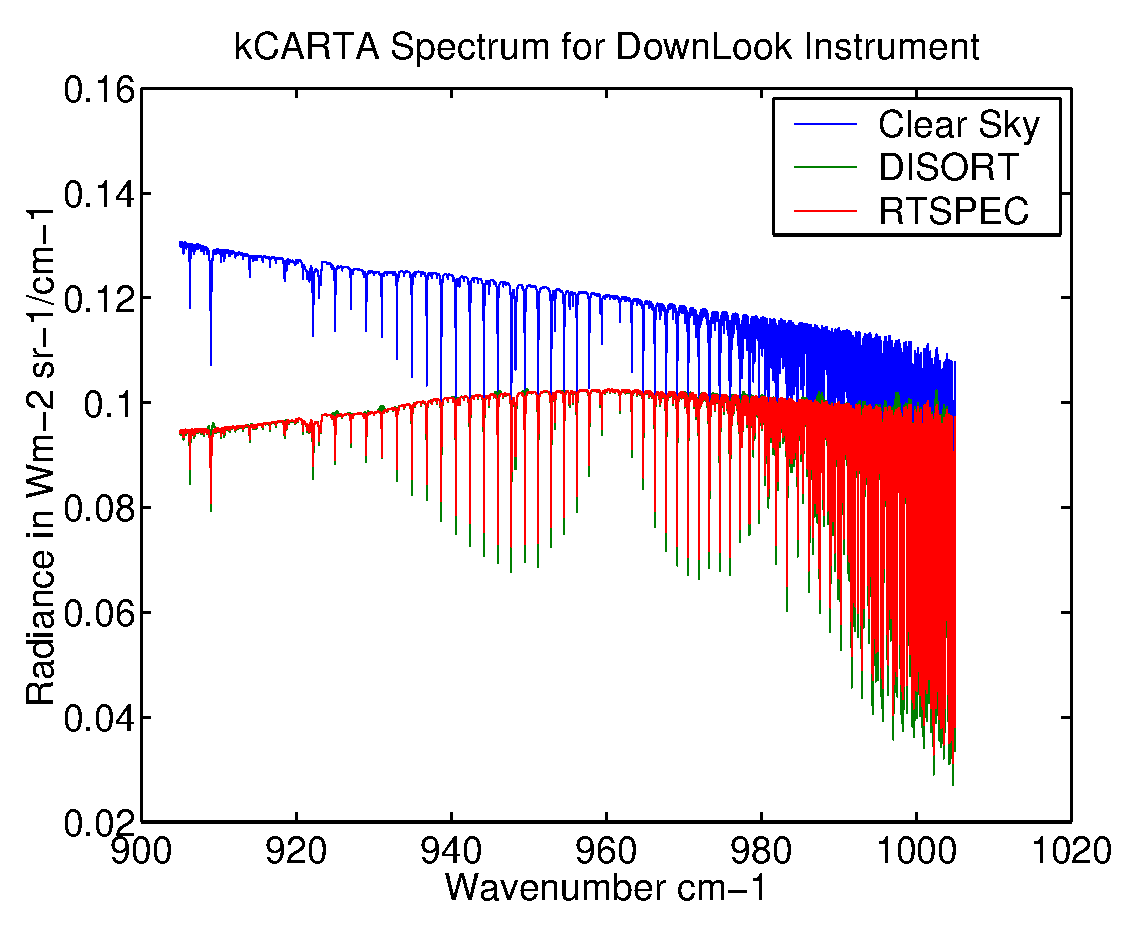
\includegraphics[width=5.5in]{FIG/show2.eps}
\caption{Sample output radiance spectrum.}
\label{sampleplot}
\end{figure}

Plotted next in Figure ~\ref{samplerads}, the clear sky radiative transfer 
algorithm was used to produce a radiance plot. 
\begin{figure}
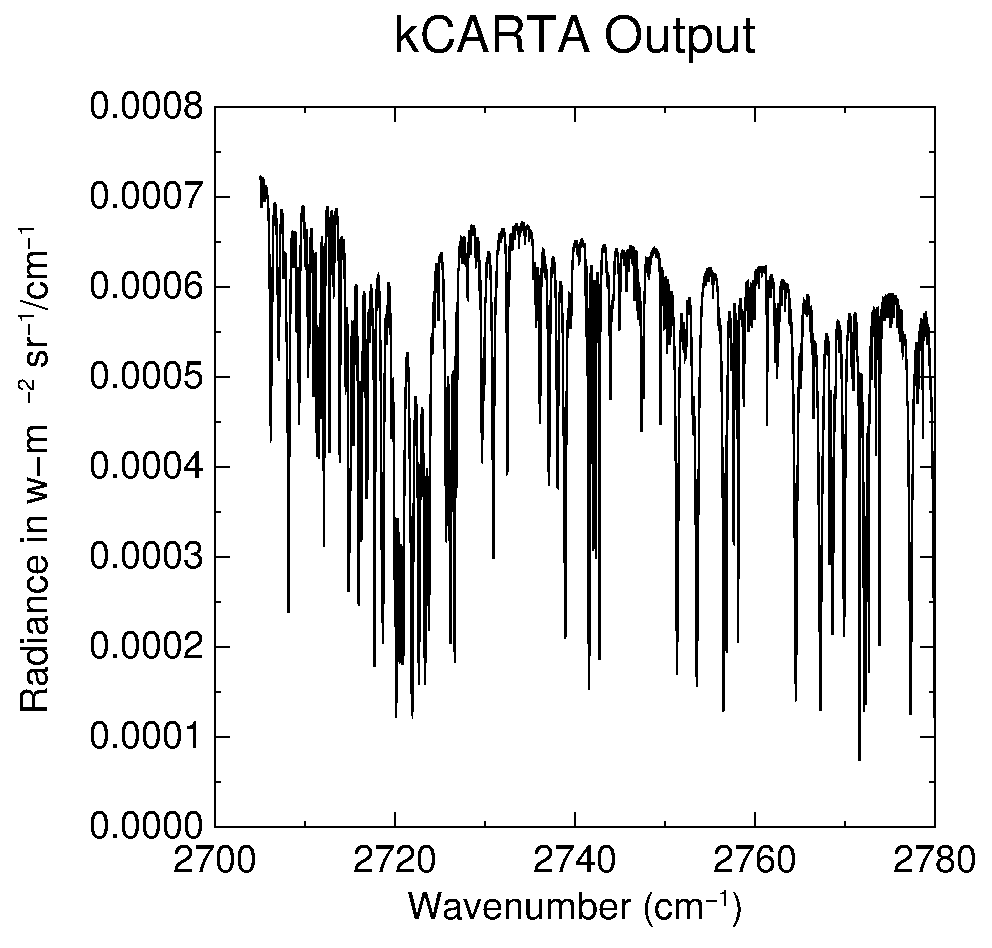
\includegraphics[width=5.5in]{FIG/show.eps}
\caption{Sample output radiance spectrum.}
\label{samplerads}
\end{figure}

\section{New Spectroscopy used by \kc}
Most of the compressed optical path database that is used by \kc, is generated
by our own custom line-by-line code. This code is based on $GENLN2$. The main
differences between our code and $GENLN2$ are
\begin{itemize}
\item $GENLN2$ divides the lines into ``near'' and ``far'' bins, while our
      code also uses a ``medium'' bin
\item Our code uses Q branch line mixing, as well as P and R branch line mixing
      for the 4 and 15 micron CO2 optical depths
\end{itemize}

Some other features of the spectroscopy used by \kc also include our 
modifications to the water-self and -foreign continuums in the 1600 \wn 
bandhead. CKDv2.4 currently underestimates the continuum contribution in this 
region.

The spectroscopy used by \kc has been validated by comparing to data from 
campaigns such as CAMEX-1, WINTEX, ARIES and CLAMS. This variety means a 
number of different instruments, in differing atmospheric situations, all seem
to imply that \kc is generally correct. In addition, we are now using data from
the AIRS instrument, which is further helping us refine some of our 
spectroscopy. For example, we had previously noted that while the linemxing 
in the 15 micron region gave us very acceptable obs-calcs, there had always 
been a little trouble in the 4 micron bandhead. The AIRS data is helping us 
further refine our model, and we hope to come out with some updated corrections
to the database very soon.

\section{Units and Definitions}

While reading this section, the user is reminded that \kc uses the 100
AIRS layers, spline interpolated onto MYNLAY layers. All angles set in the 
\kc files should be in degrees.
Frequencies are in units of wavenumbers (\wn).  In defining the
atmospheres inside the $nm\_radnce$ section, pressure boundaries should be
in millibars (1.0 atm=1013.25 mb).  Surface and deep space temperatures
are in Kelvin.  If the user specifies pressures at which radiances are
to be output, they should also be in millibars.

The gas profiles expected by \kc use the following units.  The gas
amounts are path averaged over the layers, and are in units of
$\hbox{\em kiloMoles} \cm^{-2}$.  Temperatures should be
specified in {\em kelvin}, while pressures and partial pressures
should be expressed in {\em atmospheres}.  Layer altitude
(approximately at center of the layer) should be in {\em
kilometers}.  Each gas will have a kProfLayer layer profile.  Note that if
the user inputs a point profile in the appropriate format to our
supplied {\sf kLayers} program, the path averaged profile that is
output by this program will be in the correct units.

Output gas and mixed path optical depths are dimensionless (absorption
coefficient $\times$ gas amount); obviously so are transmittances.
Output radiances are in blackbody radiance units ($\hbox{\em milliwatts}
\;\ m^{-2} sr^{-1}/\cm^{-1}$).  Jacobians can be output in one of three
modes : an example is $d(\hbox{\em rad})/ds_{m}$, where $s_{m}$ is the
temperature or gas amount in layer $m$. Fluxes are output in one of two 
modes : radiance * angle units, or $K day^{-1} /cm^{-1}$

The following terms will be found in various places throughout the document.
\begin{longtable}{|l|p{\colwidth}|}
\caption{Glossary of terms used in document}\\
\hline
compressed   coefficients & \kc uses a compressed database to quickly 
determine the absorption coefficients of most gases in the {\sf HITRAN} 
database, for the required profile\\ \hline
xsec  database & Some of the gases in the {\sf HITRAN} database (notably the 
{\em CFCs}) are too complex to have their parameters determined 
experimentally. The absorption coefficients for these gases are computed by 
interpolating the measured coefficients at various temperatures and 
pressures\\ \hline
kMaxLayer & this is the number of AIRS layers that were used in producing the
            kCompressed Database (=100)\\ \hline
kProfLayer & our $kLayers$ code allows the user to subdivide the lower AIRS 
             layers or clump together the upper AIRS levels. This means the 
             resulting number of layers could be lesser or greater than 
             kMaxLayer, depending on how klayers.x is set up. This will be 
             the actual maximum number of layers in each atmosphere for the 
             particular \kc run   \\ \hline
$nm\_params$ & some required parameters have default values.  The user can 
              change these values to other allowed values. Note these settings
              apply to the entire run.  For example, if the user chooses to 
              use water continuum version CKDv2.1, this will be used for all 
              the mixed paths and atmospheres in the run.\\ \hline
$nm\_molgas$ & required section in \kc driver namelist file.  This specifies 
              which gases need to have their optical depths computed using the
              compressed database\\ \hline
$nm\_xscgas$ & optional section in \kc driver namelist file.  This specifies 
               which gases need to have their optical depths computed using
               the cross-sectional database (xsec)\\ \hline
path         & the optical depth for a gas, in a particular layer.
               Each gas will have kProfLayer paths associated with it. If 
               there are iNGas gases specified in $nm\_molgas$, and iXsec 
               gases specified in $nm\_xscgas$, there will be a total of 
               kProfLayer(iNgas+iNXsec) paths\\ \hline
$nm\_prfile$ & required section in \kc driver namelist file.  This specifies 
              which gas  profile to use in the run. The profile would be in 
              the $kLAYERS$ output format. Each layer for each gas in this 
              profile will constitute a gas path.\\         \hline
$nm\_weight$ & required section in \kc driver namelist file.  This specifies 
               the gas weightings (one weight per gas).  This is a multiplier 
               to the gas profile, applied equally to the gas in ALL 
               $kProflayers$. \\ \hline
mixed path & When the paths for one gas are computed, as determined by the gas
             profile, the user can then combine different weights of this
             gas, with the optical depths of other appropriately weighted
             gases.  In this way, the user can build up an atmosphere that
             consists of the gases specified in $nm\_molgas$ and $nm\_xscgas$, 
             weighted appropriately. 
           As the paths are in sets of $kProfLayers$, so the mixed paths are 
           also in sets of $kProfLayers$\\ \hline
mixing table & is a term used to describe how the weightings of various
             gases (from $nm\_weight$) are added together cumulatively to
             obtain a set of mixed paths\\ \hline
atmosphere & Once the individual gas absorption coefficients have been
        combined to form sets of mixed paths (kProfLayers mixed paths per 
        set), an atmosphere can be defined from any one of the sets.
        In addition, the boundary conditions of the atmosphere (start
        and stop pressures, surface temperature and emissivity) and the
        direction of radiation travel define individual atmospheres.\\ \hline
$nm\_radnce$ & optional section in \kc driver namelist file.  Once the user 
               has combined individual gas paths to form mixed paths, he/she 
               can now define an atmosphere, as above. The radiance measured 
               by an instrument anywhere within the boundaries of the 
               atmosphere, can be calculated.  The boundary conditions (eg 
               surface temperature, upper and lower pressure boundaries) and 
               direction of radiation travel are amongst other parameters the 
               user specifies here\\ \hline
$nm\_jacobn$ & optional section in \kc driver namelist file.  Once the user 
              has defined an atmosphere, the sensitivity of the measured 
              radiance to gas amounts and temperatures of the different 
              layers can be 
              studied by computing the Jacobians and weighting functions. Note
              these sensitivities are for clear skies only. At present, the 
              code does not allow the user to compute radiances using 
              scattering models, and then compute jacobians.
              In addition, since the code computes temperature jacobians while
              it is uncompressing the kCompressed Database, it cannot compute
              these jacobians if the spectra for some gases in a wavenumber
              interval are externally supplied.\\ \hline
$nm\_scattr$ & optional section in \kc driver namelist file.  Once the user 
               has defined an atmosphere, by default, radiance computations 
               will assume a clear sky.  However, the user can choose to 
               include various clouds in each atmosphere, and use our 
               interface to the scattering codes such as $rtspec.f$, 
               $disort.f$ or $twostream.f$ or $pclsam.f$ . If scattering is 
               turned on, then jacobians will be be computed using the 
               $pclsam$ algorithm.\\ \hline
$nm\_nonlte$ & optional section in \kc driver namelist file.  Once the user 
               has defined an atmosphere, by default, radiance computations 
               will assume a clear sky in LTE.  However, the user can choose 
               to include NONLTE computations for some of the upper layers of
               the AIRS atmosphere. Since this entails doing laborious line by
               line computations, the code slows down tremendously!\\ \hline
$nm\_spectr$ & This section allows the user to choose more than one gas, and 
              have  kCARTA read in LBL spectra produced by some other code
                for defined spectral regions. These regions have to overlap 
                the kCARTA chunks eg 705-730, 1255-1280 etc
                If this option is used, then $nm\_jacobn$ cannot be used!!
                Also, the code will simply read in the spectra, and weight it
                appropriately ... it will not do checks . In other
                words, it is the users responsibility to make sure the
                spectra read in were computed with the correct layer amounts
                and temperatures.\\ \hline
$nm\_output$ & required section in \kc driver namelist file.  The user can 
            choose to output path or mixed path spectra, or radiances\\ \hline
$nm\_endinp$ & required section in \kc driver namelist file.  Specifies end of 
         driver namelist file\\
\hline
driver namelist file & this namelist file contains settings that are read in 
            by  \kc  and then control the running of the code 
            (namely, what output to produce)\\ \hline
iNatm     & number of atmospheres defined in driver namelist input file\\ 
            \hline
\end{longtable}

\subsection{Note about computed fluxes}
Here our definition of flux is integration of the upward radiance over 
incident angles minus integration of downward radiance over incident angles,
at each boundary pressure level in the atmosphere. The difference between the
upward and downward ``fluxes'' then give us the net heating of the layer, 
which is directly related to the temperature change per unit time.  Refer to 
Liou,  ``An Introduction to Atmospheric Radiation'', pg 107. If the 
atmosphere is defined between layers 3 and 65, then the flux differences 
(at 0.0025 \cm resolution) between the top and bottom of each of layers 
3-65 is output. In other words, the code does not sum over all the radiances 
across the infrared spectrum, but just outputs the monochromatic ``flux''. The
user will read in this flux, and ``add all the points, multiplied by 0.0025.''

If the user supplies a name $filename$ for the usual radiance 
results to be output, then the flux results (kFLux = 1,2) are in 
$filename\_FLUX$ (or if kFLux = 3,4 $filename\_OLR$); otherwise
they will stored in flux.dat. Note that if kFlux=1,2,3,4 and if a radiance for
an atmosphere is to be output, then the fluxes will be computed. This is 
independent of whether or not Jacobians are to be computed. 

If kFlux=1, the fluxes are simply an integral of radiance over 
$2 \pi \mu d\mu$, which means the units will be radiance units $\times$ s
teradians, or mW m-2/cm-1. 

If kFlux=2, the fluxes are an integral of radiance over $2\pi \mu d\mu$, and 
then divided by $-c_{p} \;\; \rho \delta z$ where $c_{p}$ is the specific heat
at constant pressure, $\rho$ is the density and $\delta z$ is the layer 
thickness. This means the units will be $Kelvin$ per $day$ per$cm^{-1}$. 

To get the same type of plots that are in Liou, ``An Introduction to 
Atmospheric Radiation'', pg 108, the user first has to read in the computed 
``fluxes''; then for each layer, 
\textcolor{red}{sum across the monochromatic ``fluxes'', multiply the result 
by 0.0025 $cm^{-1}$} (as this is the same as integrating $I(\nu) d\nu$) to 
get the correct flux units (the factor of 86400 has already been accounted 
for, so the units are ``correct.''). 

If kFlux=3, only outgoing radiation at the top of each layer is computed; so 
the units are the same as for kFlux=1 case, namely  mW m-2 per wavenumber 
point. If the user is only interested in OLR at the top of the atmosphere, 
then kFlux=4 only outputs upgoing flux at TOA (thus making the binary output 
files approximately 100 times smaller than fluxes outout at $all$ layers).
For kFlux = 3,4
\textcolor{red}{don't forget to multiply by d(nu) = 0.0025 cm-1 
                when doing the (Matlab) integral over frequency (and divide 
                the result by 1000 to change from mW to W if kFlux = 1,3)!!!!}


A sample flux plot is shown below, in Figure ~\ref{sampleflux}

\begin{figure}
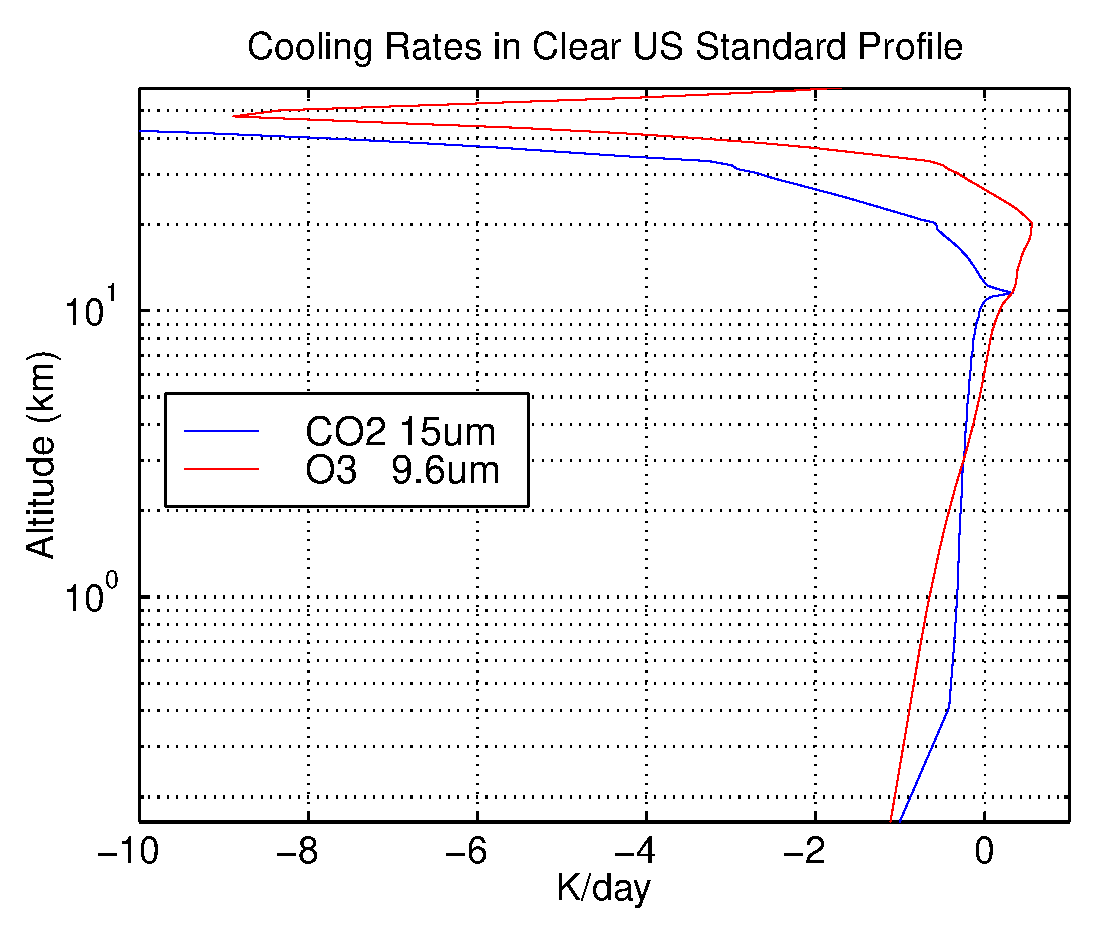
\includegraphics[width=5.5in]{FIG/coolrate.eps}
\caption{Sample flux computation.}
\label{sampleflux}
\end{figure}

\section{Using KLAYERS : change point profile to layer averaged profile}
See the KLAYERS documentation. It is supplied to default to the AIRS 100 layers
but the user can rest the pressure levels as necessary.

\subsection{Compiling kcarta}
Once the user has successfully run klayers.x as described above, he/she should
now go to the kCARTA/SRC directory. 

The user now has to edit kcarta.param, and set kProfLayer to the same number 
of layers that $klayers.x$ can produce. Having 
done this, \kc is ready to be compiled (type ``make'') and then run.

\section{Using RTSPEC : producing the Mie Scattering tables}
If the user only wants to compute clear sky radiances, then this section can 
be skipped. However, this section must be read by someone interested in using
\kc for scattering computations. 

To do scattering computations, \kc has been interfaced with two extensively
tested scattering routines : $RTSPEC$ and $DISORT$. While $RTSPEC$ 
\footnote{ M.~N.~Deeter and K.~F.~Evans, ``A Hybrid Eddington Single 
Scattering Radiative Transfer Model for Computing Radiances from Thermally 
Emitting Atmospheres,'' {\em JSQRT} {\bf 60} 635-648 (1998)}
is very fast, it cannot be used when one has a beam source present 
(eg a solar beam). $DISORT$ 
\footnote{ K.~Stamnes, S-C.~Tsay, W.~Wiscombe and K.~Jayaweera, ``Numerically
Stable Algorithm for discrete ordinate method Radiative Transfer in multiple
scattering and emitting layered media,'' {\em Appl. Opt} {\bf 27}, No 12, 2502
(1988)} can handle this case; however it is much slower than $RTSPEC$. We have
written our own $TWOSTREAM$ code that is fast and allows the user to use a
solar beam. In addition we now have an interface to $PCLSAM$ which also 
allows the use of solar beam, and is very fast. Jacobians and fluxes can easily
be computed with this algorithm.

To combine the advantages of both of these well documented and tested 
scattering codes, \kc has been interfaced to both these codes so that the 
same information is needed for either scattering routine. As $RTSPEC$ needs
some more specific information, we have chosen to include the scaled Mie
properties computed by the sister code to $rtspec.f$, $sscatmie.f$. Given
some general inputs, this code will compute extinction coefficients, single 
scattering albedos and asymmetry parameters that can be used by both codes,
for ice or water clouds.

In addition, we have extended the capability of $sscatmie.f$ by interfacing
the aerosol package $OPAC$ 
\footnote{M.~Hess, P.~Koepke and I.~Schult, ``Optical Properties of Aerosols 
and Clouds : The Software Package OPAC,'' {\em Bull. Am. Met. Soc}, {\bf 79}, 
No 5, 831 (1998)} to it. The addition of this database extends the 
capabilities of $sscatmie.f$ to compute the same parameters 
for a variety of aerosol modes, at varying relative humidity values.

The original source code and documentation for some of the packages is 
easily obtained over the Internet : \\
\begin{verbatim}
RTSPEC : http://nit.colorado.edu/~evans/rtspec.html
DISORT : ftp://climate.gsfc.nasa.gov/pub/wiscombe/Multiple_Scatt/DISORT2.0beta/
OPAC : http://www.lrz-muenchen.de/~uh234an/www/radaer/opac.html
\end{verbatim}

To produce the Mie scattering tables, go to the $../SCATTERCODE/RTSPEC$ 
directory. Type ``make'' at the prompt to compile the code (at present the
code has been tested on SGI Ultrix and Absoft F77 Linux).
This should produce 5 executables :\\
\begin{itemize}
\item combine : this allows the user to ``combine'' a number of text output
                Mie files, into one single binary file
\item translate : this allows the user to ``translate'' a text output
                Mie file, into a smaller binary file
\item rtspec : the compiled ``rtspec'' code
\item SSCATMIE : this is the executable the user will use to generate Mie
                 scattering tables of ice, water clouds or aerosols
\item refind : the user can use this to compute refractive indices of ice, 
               water clouds or aerosols
\end{itemize}

The particle distribution assumed by $sscatmie$ is a modified gamma 
distribution, where the user can vary parameter $\alpha$ (typically = 6): 
\[
n(r) = \gamma r^{\alpha} exp^{-br}
\]
The peak of the distribution is at $x = \alpha/b$. Both $b$ and $r$ are in 
microns. The normalization term $\gamma$ is related to the liquid water 
content $\rho_{lwc}$ by
\[
\rho_{lwc} (g m^{-3}) = \int (4/3)\pi r^3 \rho_{water} n(r) dr = 
\gamma  \frac{4 \pi}{3} \rho_{water} \frac{\Gamma(\alpha+4)}{b^{\alpha+4}}
\]
while the average or effective radius of the distribution is given by
\[
r_{avg} = \frac{\int n(r) r^3 dr}{\int n(r) r^2 dr} = \frac{\alpha+3}{b} = Dme
\]
Depending on the grid of particle sizes chosen (see {\em Enter min and max 
Dme, and number of sizes} below), this are the values at which $sscatmie$ 
reports results. 

As $sscatmie$ runs, it prompts the user to answer the follwoing questions :
\begin{verbatim}
 Enter filename for output table
 Fixed wavenos or evenly-spaced wavenos (F or E):
 Enter min, max and number of wavenumbers (cm^-1)
 Enter min and max Dme, and number of sizes
 Enter alpha for particle distribution
 Enter species ('I'=ice, 'W'=water, 'A'=aerosol):
 If aerosol, 
   Enter aerosol type and Relative Humidity
        0 : General NH4SO4, from Remote Sensing of Atm by G. Stephens
        1 : OPAC INSO : insoluble aerosol
        2 : OPAC WASO : water-soluble aerosol
        3 : OPAC SOOT : soot
        4 : OPAC SSAM : sea salt (accr mode)
        5 : OPAC SSCM : sea salt (coag mode)
        6 : OPAC MINM : mineral salt (nucleated mode)
        7 : OPAC MIAM : mineral salt (accr mmode)
        8 : OPAC MICM : mineral salt (coag mode)
        9 : OPAC MITR : mineral transported (desert dust)
       10 : OPAC SUSO : sulphate droplets
 Enter cloud temperature (Kelvin)
 If ice or aerosol
   Enter Volume fraction factor (a) and exponent (b) (vf=a*D^b, D in um)
 Enter E for evenly-spaced mu or Q for Lobatto-Quadrature mu
 Enter min and max mu, and number of angles
 Delta scale the scattering properties (Y, N, H, or G)
\end{verbatim}

Typical answers for an atmosphere with sulphate droplets aerosol, are
\begin{verbatim}
/CLOUDS/aerosol.scatab805     !output file name
'E'                           !evenly spaced wavnos
805.0 1005.0 50               !start,stop waveno
0.1 100 10                    !particle sizes
6                             !alpha parameter, for the particle size distr
'A'                           !aerosol   
 10  30.0                     !sulphates (OPAC file 10), at 30%RH
230.0                         !cloud temp (irrelevant)
1.0 0.0                       !volume fraction and exponent
'E'                           !evenly spaced mu (cos(x)) for quadrature
0.1 1.0 10                    !min(mu),max(mu) ... used by RTSPEC
'G'                           !delta scale to make things more accurate
\end{verbatim}

Typical answers for a cirrus cloud in the troposphere (~11 km), are
\begin{verbatim}
/CLOUDS/ice.scatab805         !output file name
'E'                           !evenly spaced wavnos
805.0 1005.0 50               !start,stop waveno
0.1 100 10                    !particle sizes
6                             !alpha parameter, for the particle size distr
'I'                           !aerosol   
230.0                         !cloud temp (irrelevant)
1.0 0.0                       !volume fraction and exponent
'E'                           !evenly spaced mu (cos(x)) for quadrature
0.1 1.0 10                    !min(mu),max(mu) ... used by RTSPEC
'G'                           !delta scale to make things more accurate
\end{verbatim}

The files produced by running the code can now be used by \kc

\section{\kc source files}
This section gives a brief description of the different files containing the
source code for \kc.

\begin{itemize}
\item this set of continuum and cross section files will eventually be phased
out, as we are moving towards using a kCompressed style format for the 
cross section gases, and a lookup table format for the CKD computations.
\item {\sf calcon*.f} : compute the water continuum (CKD v0,1,2,2.3,2.4 etc)
\item {\sf calq.f}    : auxiliary file to compute cross-section absorption 
                        coefficients (gas IDs 51-63)
\item {\sf calxsc.f}  : file to compute cross-section absorption 
                        coefficients (gas IDs 51-63)

\item {\sf freqfile.f}        : kCARTA start/stop chunks, other misc stuff
                                eg database freq checks for given gas/chunk
                                combos and so on
\item {\sf rtp\_interface.f}   : interface with RTP libraries
\item {\sf spline\_and\_sort.f} : lots of functions; sorting, splines, mod, 
                                  div,real2double etc

\item {\sf h2oft0.f} : water continuum data blocks, GENLN2 (lorentz) style
\item {\sf h2ost0.f} : water continuum data blocks, GENLN2 (lorentz) style
\item {\sf h2ost1.f} : water continuum data blocks, GENLN2 (lorentz) style
\item {\sf h2oft0\_wb.f} : water continuum data blocks, correct (local) style
\item {\sf h2ost0\_wb.f} : water continuum data blocks, correct (local) style
\item {\sf h2ost1\_wb.f} : water continuum data blocks, correct (local) style

\item {\sf rad\_main.f} : clear sky radiance calculations
\item {\sf rad\_diff.f} : compute thermal background using diffusivity approx
\item {\sf rad\_quad.f} : compute thermal background using quadrature
\item {\sf rad\_misc.f} : solar and other misc radiance code
\item {\sf rad\_flux.f} : clear sky flux code

\item {\sf scatter\_rtspec\_main.f} : interface to RTSPEC calculations
\item {\sf scatter\_rtspec\_code.f} : RTSPEC scattering code (from Frank Evans)
\item {\sf scatter\_rtspec\_flux.f} : flux code (totally incomplete!!!!)

\item {\sf scatter\_pclsam\_main.f} : interface to PCLSAM calculations
\item {\sf scatter\_pclsam\_code.f} : PCLSAM scattering code 
\item {\sf scatter\_pclsam\_flux.f} : flux code

\item {\sf scatter\_disort\_main.f} : interface to DISORT calculations
\item {\sf scatter\_disort\_code.f} : DISORT scattering code (from K. Stamnes)
\item {\sf scatter\_disort\_misc.f} : couple of DISORT specific routines
\item {\sf scatter\_disort\_flux.f} : flux code (totally incomplete!!!!)

\item {\sf scatter\_twostream\_main.f} : interface to TWOSTREAM calculations
\item {\sf scatter\_twostream\_code.f} : twostream scattering code 
\item {\sf scatter\_twostream\_guts.f} : twostream scattering code (contd)
\item {\sf scatter\_twostream\_flux.f} : flux code 

\item {\sf jac\_main.f} : main jacobian code
\item {\sf jac\_up.f} : jacobian code for up looking instrument
\item {\sf jac\_down.f} : jacobian code for down looking instrument

\item {\sf kcartamain.f} : main \kc source file
\item {\sf kcartamisc.f} : misc routines eg splines

\item {\sf kcoeffMAIN.f} : set up calls to compute LTE absorption coefficients
\item {\sf kcont\_xsec.f} : set up calls to compute continuum, xsec
\item {\sf kcoeffSPL.f}  : compute LTE absorption coefficients
\item {\sf kcoeffSPLJAC.f}  : compute LTE absorption coefficients, do Jacobians

\item {\sf knonlte.f} : set up calls to compute NLTE absorption coefficients
\item {\sf klineshapes.f}  : computes qfncs, lte line strengths etc for NLTE 
                             absorption coefficients; optimized for 4 um CO2 
                             region, and also reads in HITRAN parameters
\item {\sf kreadVTprofs.f} : reads/writes GENLN2 styles vib temp files
\item {\sf kpredictVT.f}   : tries to predict NLTE profs and writes out GENLN2
                             style vib temp files
\item {\sf kvoigt\_cousin.f}  : computes voigt and cousin lineshapes
\item {\sf kcousin.f}         : computes co2 continuum and cousin lineshapes

\item {\sf n\_main.f} : main input file parsing routines 
\item {\sf n\_gas\_spectra.f} : MOLGAS,XSCGAS,SPECTRA,NLTE parsing routines 
\item {\sf n\_pth\_mix.f} : PTHFIL,MIXING  parsing routines 
\item {\sf n\_rad\_jac\_scat.f} : RADFIL,JACOBN, SCATTER parsing routines 
\item {\sf n\_output.f} : OUTPUT parsing routines 

\item {\sf s\_writefile.f} : output writing routines 
\item {\sf s\_misc.f} : misc parsing routines and readers
\end{itemize}

\section{Required data files}

\kc requires a number of data files to be present at compile time, and
another set to be present at run time.  At compile time, the required files 
contain definitions for the array sizes, as well as the paths to the 
database and required files. 

At run time, the various required files drive the run-time session of the 
program, tell it which compressed data files exist for which gas, in different
wavenumber regions, and so on.  Thus, some of these files will have to be
regenerated by the user each time he/she updates the compressed
database.  In particular, the program compdatabase.f, in subdirectory
{\sf UTILITY} (along with the script comp.sc that exists in
subdirectory {\sf SCRIPTS}) should be run each time the user updates
the files that exist in the compressed database.  A summary of the
existing database files then exists in {\sf comp97.param}.

The following parameter files need to be present at compile time,
in the same subdirectory as the source code.

\begin{small}
\begin{longtable}{|l|p{\colwidth}|}
\caption{Compile time parameter files.}\\
\hline
kcarta.param        & compile time file that allows the user to define the
                      paths to compressed database, reference profiles etc
                      In addition, the user can define the size of matrices,
                      arrays and so on here\\ \hline
gauss.param         & contains Gauss-Legendre wieghts for angular 
                      integrations\\ \hline
scatter.param       & contains interface array dimensions kCARTA to scatter 
                      code\\ 
pre\_defined.param  & contains many interface array dimensions for kCARTA; 
                      DO NOT TOUCH!!!!\\ 
post\_defined.param & contains many interface array dimensions for kCARTA; 
                      DO NOT TOUCH!!!!\\ 
\hline
\end{longtable}
\end{small}

\noindent The following data files need to be present at run time, in the
relevant subdirectory specified in {\sf kcarta.param}.  (If no cross-section 
gases are to be used, then {\sf xsec.param} is not necessary)\\
\begin{small}
\begin{longtable}{|l|p{\colwidth}|}
\caption{Run time data files.}\\
\hline
comp97.param  & contains a summary of the compressed database, so the
                program knows which gas absorption coefficients can be
                uncompressed for a particular frequency range\\ \hline
xsec.param    & contains a summary of the crosssection database, so the
                program knows which {\sf CFC} absorption coefficients can be
                included for a particular frequency range.
                Note that currently there is a switch between using the H92
                cross section database, or using the H98 kCompressed files for
                these gases; this will be phased out eventually.\\
                \hline
\end{longtable}
\end{small}


Of the following data files, only the driver namelist input file and the 
profile need to be present at run time, in the relevant subdirectory chosen 
by the user. Depending on the set of instructions found in the driver 
namelist file, the last two files may or may not be needed.\\
\begin{small}
\begin{longtable}{|l|p{\colwidth}|}
\caption{Other data files.}\\
\hline
driver namelist file & contains user specified Gas ID's, frequency range
            gas weights, atmosphere definitions, output styles, etc.
            This is the main file that drives the running of \kc\\ \hline
gas profile & contains the path profile information (gas amounts,
            pressures, partial pressures, temperatures and so on.
            kProfLayers layers are required for each gas.
            User can opt to use a shorter version (water and ozone 
            amount/temperature profiles), or just use read in a 
            regression profile.
            NOTE the gas profile can either be in the old KLAYERS format, 
            which is a text file, or in the new RTP format\\ \hline
continuum  & we are using our own set of lookup tables for the water
             continuum. These tables are based on the CKDv0,21,23,24 tables,
             as well as CKD 51,55 which are our own modifications\\ \hline
emissivity  & if radiances are to be computed, the user can vary the
            surface emissivity as a function of wavenumber.
            NOTE If a RTP file is used to read in atmospheric info as well,
            this file will also include the emissivity and solar reflectivity\\
            \hline
xsecdata  & if the absorption coefficients of the {\em CFC's} are to be
            included, and the user wants to use the old H92 cross sections
            data, the file containing this info must be present. the user needs
            to set  kXsecFormat = -1 in the kcarta.param file 
            We supply file xsecdata.dat in {\sf DATA/General}.
            Note that this requirement has been phased out, as the user can 
            use a kCompressed style format for the cross section gases, by
            setting  kXsecFormat = +1  in the kcarta.param file\\ \hline
\end{longtable}
\end{small}

A partial listing of the parameter file {\sf comp97.param} is\\
\begin{center}
\begin{small}
\begin{longtable}{cccc}
\caption{Parameter file listing.}\\
  1 &    605.000000 &    2830.000000 & 2\\
  2 &    605.000000 &    1105.000000 & 2\\
  2 &   1205.000000 &    1405.000000 & 2\\
  2 &   1830.000000 &    2555.000000 & 2\\
  2 &   2580.000000 &    2655.000000 & 2\\
  2 &   2730.000000 &    2780.000000 & 2\\
  3 &    605.000000 &     880.000000 & 2\\
\end{longtable}
\end{small}
\end{center}
where the first column denotes the ({\sf HITRAN}) GasID, and the second/third 
columns the start/stop frequencies of the compressed database coverage of 
that gas. The fourth column indicates these files are of type ``2''
which all have a wavenumber spacing of 0.0025 \wn. 
The only gases/frequency combinations stored in the database are 
those that have appreciable cross sections for an Earth atmosphere.

When the program starts to run, it checks to ensure that the parameters set 
in {\sf kcarta.param, pre\_defined.param, post\_defined.param} make sense.  
It then parses in the
driver namelist file, and if necessary the gas profile.  After this, the 
program starts running in earnest, making use of files {\sf comp97.param,
  xsec.param} and {\sf xsec.data} when necessary.

%A flow diagram is shown below.
%\begin{center}
%\begin{picture}(360,560)
%\thicklines
%\put(110,550){\framebox(140,50){kcarta,airslevels.param}}
%\put(125,445){\framebox(110,60)}
%\put(130,450){\framebox(100,50){compile \bf kCARTA}}
%\put(10,250){\framebox(100,50){input namelist file}}
%\put(10,150){\framebox(100,50){gas profile?}}
%\put(10,50){\framebox(100,50){emissivity?}}
%\put(250,250){\framebox(100,50){comp97.param}}
%\put(250,150){\framebox(100,50){xsec.param?}}
%\put(250,50){\framebox(100,50){xsecdata.dat?}}
%\put(130,50){\framebox(100,260){parser}}

%\put(180,550){\vector(0,-4){45}}
%\put(180,445){\vector(0,-4){135}}
%\put(180,50){\vector(0,-4){45}}
%\put(60,200){\vector(0,4){50}}
%\put(300,100){\vector(0,4){50}}

%\put(110,275){\vector(4,0){20}}
%\put(250,275){\vector(-4,0){20}}
%\put(250,175){\vector(-4,0){20}}
%\put(110,75){\vector(4,0){20}}

%\end{picture}
%\end{center}

\section{Compile time file {\sf kcarta.param}}

Before compiling the code, the user has to tell \kc what size arrays
and matrices are to be declared, as well as the paths to required
files, such as those in the compressed database and the reference and
regression profiles.  This is done by setting various parameters in
file {\sf kcarta.param}, which is divided into 2 sections.  The first
section has the set of user defined parameters.  How to set up this
section of the file has to be thoroughly understood, as the parameters
set in the {\sf kcarta.param} file determine where the programs
searches for the compressed database, as well as allocating memory.
Any errors here will likely cause the program to stop execution. The
second section of the file contains other definitions and parameters
and should NOT BE TOUCHED (if they are, insert usual hazard messages,
use at own risk, etc., here).

Table ~\ref{kcarta.param} gives the list of user definable parameters
for this file.  Recommended settings are given in the table; the user
should not set his/her parameters indiscriminately. Note that the datafiles
that are pointed to by the paths, need to be for the correct endian versions.

%\begin{small}
%\begin{table}
\begin{longtable}{|l|p{\colwidth}|}
\caption{Setting up compile time file {\sf kcarta.param}\label{kcarta.param}}\\
\hline
kOrigRefPath & this tells kCARTA where to look for the original 100 layers
              AIRS reference profiles. One should think of this as the
              definition of the kCARTA database; it is essentially the 
              1962 US Standard Profile, tweaked slightly to reflect eg 
              increased CO2 and CH4 levels, and interpolated onto the AIRS
              100 layers (101 pressure levels) grid.\\
              \hline \hline
           & IEEE\_BE vs IEEE\_LE\\              
           & \\
kWaterPath & Path to the compressed data files for Water.\\ 
           & Typically {\sf ../DATA/WaterDataBase}\\ 
kCO2Path   & Path to the compressed data files for linemix CO2.\\
           & Typically {\sf ../DATA/CompDataBase}\\ 
kCousin\_CO2Path   & Path to the compressed data files for cousin CO2.\\
           & If available, typically {\sf ../DATA/CompDataBaseOld/}\\ 
           & If unavailable, set to {\sf ../DATA/CompDataBase/} and ignore\\ 
kCompPath  & Path to the compressed data files for RestOfGases 
             (excl water,Co2).\\
           & Typically {\sf ../DATA/CompDataBase}\\ 
kCKDPath   & Path to the CKD continuum data files (Water Self and Foreign).\\ 
           & Typically {\sf ../DATA/General/CKD}\\ 
kSolarPath & Path to the solar spectral data files.\\
           & Typically {\sf ../DATA/General/SOLAR}\\ 
kXsecFile & path to {\sf xsecdata.dat}, which stores the cross-sectional 
               cross-sectional absorption coefficients.\\
              & Typically, in DATA/Template subdirectory\\ \hline \hline
           & \\
kCompParamFile & path to {\sf comp97.param}, which stores gas ID/frequency
               span in the compressed database.\\
              & Typically, in DATA/Template subdirectory\\ 
kXsecParamFile & path to {\sf xsec.param}, which stores gas ID/frequency
               combinations in the cross-section databases.\\ 
              & Typically, in DATA/Template subdirectory\\ \hline
           & \\
kProfLayer & this is number of layers that kCARTA will do computations for.
             This parameter should be set to be the same as the number of 
             layers produced from $klayers.x$\\
kMaxAtm    & max number of atmospheres allowed. 
           Does not use too much memory, so 5 is a safe number\\ \hline
kGasStore  &  max number of gases for which kCARTA allocates storage
           (from MOLGAS + XSCGAS  $\le$  kMaxGas).  Typically, set to 38
           (25 from MOLGAS, 13 from XSCGAS) \\ 
kMixFilRows& max number of mixfil rows that can be read in.
         Remember that each set of mixedpaths has kProfLayers mixed paths. 
         Thus a safe number = kProfLayers*(number of sets you will define)
         So a forward model using four sets of mixed paths (F,FW,FWO and FO), 
         will require this number set to 4*kProfLayers\\
kMaxPrint  & max number of printing options that can be read in.  Does not use 
            too much memory, so 5(atmospheres)+2(one for gas spectra, one 
            for path spectra)=7 is a safe number. 
           Note that you should account for gas paths, mixed paths and
           radiances from EACH atmosphere as separate options\\ \hline
         & \\
kEmsRegions & max number of data points in any emissivity data file.
            This means the number of regions defined = kEmsRegions-1.
            This can typically be set to 20\\ 
kMaxDQ     & max number of gases to compute d/dq Jacobians for.
           Note that this uses up a LOT of memory.  All gases specified in
           $nm\_jacobn$ have their d/dq computed (ALL gases are used in 
           computing d/dT).  Typically, set to 2 or 3.\\ 
kProfLayerJac  & this is set to kProfLayer if the user wants to compute 
                 Jacobians while running the code, else it is set to 1\\
kMaxPtsJac  & this is set to 10000 (number of wavenumber points per 
           kCompressed chunk - see kMaxPts defined above) if the user wants to 
           compute Jacobians while running the code, else it is set to 1\\
             \hline
         & \\
kMaxClouds  & tells the code how many clouds can be used in radiance 
              computations \\
kCloudLayers  & tells the code how many layers each cloud can have\\
             \hline
         & \\
kXsecFormat   & tells the code if minor cross section gases data are in
               separate kCompressed files format (+1) or  binary file (-1).
               Will eventually be phased out as we move towards supplying only
               the kCompressed files for these gases\\
             \hline
           & \\
kBoxCarUse & tells the code how many points to BLOAT the NLTE calcs by.\\
kRegrProf  & tells the code how many regression training profiles used \\
kMaxPtsBox & tells the code how much space to save for NLTE optical depths\\
kBloatPts  & seems to be the same as kBoxCarUse, but not really; too lazy to 
             remember the difference, but I am sure there is one; probably if
             kBloatPts == 1, then this is SPACESAVER mode and so cannot
             do the bloated computations\\
caWeakCO2Path &  for each of the $N$ gases in NLTE, we now know how many 
                 chunks are in NLTE. The gas molecules have many lines/bands; 
                 some are weak and in LTE, some are strong and are in LTE, 
                 while others are strong and in NLTE. caWeakCO2Path is a path 
                 that points to a compressed databse, that has the WEAK lines 
                 in LTE precomputed. \\
kUpperAtmRefPath & path to upper atm 100 layers reference profiles. These 
                  profiles were used in making upper atm kCARTA database. \\
caWeakUpperAtmCO2Path & same as above, except it is the database for the upper
                        atm (70-120 km). Also has 100 layers x 10000 pts \\
caLineMixDir & tells the code where the CO2 4 um LineMix files are, for use in
               the LBL nonLTE computations.\\
caStrongLineParams & tells code where the CO2 4 um line parameters are, for 
               strong NLTE lines used in the LBL nonLTE computations.\\
             & Must agree with the information in caaStrongLines (see below)\\
kNLTEProfLayer & tells the code the maximum number of layers in the NLTE
                 profiles supplied by Dave Edwards GENLN2 (<= 120 right now) \\
kRegrFile & path to regression profiles that code needs if it guesses VT.
            In the nm\_nonlte section, user can give kCARTA a vib temp NLTE
            profile in variable caaNLTETemp; if the user does not do so and
            puts the name 'nlteguess', kCARTA will use a polynomial guess
            of the NLTE temps (it could also read in 48 regression profiles 
            to see which one most closely matches the current profile, and 
            then interpolate this profile in solar angle, but this is 
            a little too complicated)\\
kLOPEZPUERTAS & if kCARTA tries to put in its own vib temp profile based on 
               those from the regression profiles, it needs to know where to 
               pick up the NLTE files computed by Manuel Lopez-Puertas\\
kNLTEPolyfits & if kCARTA tries to put in its own vib temp profile based on 
               polynomial fits from the regression profiles, it needs to know 
               where to pick up the coefficients for the bands and QVs \\
               \hline
\end{longtable}

To keep memory sizes manageable, the jacobian parameter declarations in this
file might be set to ``1''. To allow \kc to perform jacobian computations, 
turn off the ``space save dimensions'' that might be in the tar package by  
simply uncommenting the lines above which these space saver dimensions are 
defined.

\section{Compile time file {\sf scatter.param}}
Here the user can prune or enlarge the arrays used by the scattering codes 
$DISORT$, $RTSPEC$, $TWOSTREAM$ $PCLSAM$. This will have major consequences on
the amount of memory used when
running \kc. However, it it probably safer to use the param file as it is. We
might supply the tar package with the ``space save dimensions'' turned on; 
variables maxcly, maxulv,mammon etc might be set to 1; if so simply uncomment
the lines above which these space saver dimensions are defined, to turn on
the parameter value that $DISORT$ can work with.

\section{The Driver Namelist File}

At present, our kCompressed database spans the wavenumber range from 
605 \wn to 2805 \wn, with a point spacing of 0.0025 \wn. kCARTAv0.97+ has
been written so that planned future extensions to the database can be 
easily handled by this current version. (The planned extensions are from
about 250 \wn to 605 \wn, and will need a higher resolution than  0.0025 \wn).
Note that the program has been written so that the user cannot ``mix'' regions
that have different wavenumber point spacings. In other words, if the starting 
frequency is such that the corresponding file has a wavenumber spacing of 
0.0001 \wn, and the stop frequency is such that the corresponding file has a 
wavenumber spacing of 0.0025 \wn, the program will stop.

This section gives the structure of the namelist file that controls the 
running of \kc.  Note that 
\begin{itemize}
\item {\bf IMPORTANT} Each run of \kc involves one driver namelist file.
  Within this file, the user can either read in his own profile, or
  use one of the supplied regression files.  Thus one \kc run can only
  use one profile.
\item At present the absorption spectra for the minor cross section gases can
  be computed by either using a binary file containig all HITRAN92 data, or by
  reading in kCompressed files for these gases. This is controlled by
  parameter kXsecFormat above (set to -1 in kcarta.param distribution)
\item While the code does allow one to compute the radiation measured
  by an upward looking instrument, at present even the bottommost
  layers are probably too coarse for an accurate estimate. Using our new 
  kLAYERS code, the bottom AIRS layers can be subdivided finely, or the 
  topmost layers can be clumped together. In
  addition, if the user wants the sun to be included in the FOV of the
  instrument, the program does not compute the variation in the local
  solar angle; at present, it simply uses the variation in the local
  path angle.  We will be working on fixing these issues in the future.
\item While reading this section, it might be helpful to look at the
  sample template files in {\sf ../DATA/TemplateNML} subdirectory.  In
  addition, the following points should be remembered :
   \begin{itemize}
   \item the namelist file is divided into about 12 separate sections. For
      example, $nm\_prfile$ contains the profile name, while 
      $nm\_frqncy$ contains the start and stop frequencies.
   \item if at most the profile is driven by an RTP file (kRTP = -2,-1,0) then 
         keywords MOLGAS, FRQNCY, PRFILE, OUTPUT are required  
   \item if the RTP file drives almost everything (kRTP = 1) then 
         keywords MOLGAS, PRFILE, OUTPUT are required  
  \item keywords PARAMS, XSCFIL, WEIGHT, RADNCE, JACOBN, SCATTR, NONLTE, 
        SPECTRA are optional 
   \item comment lines begin with !, character strings enclosed in quotes
   \end{itemize}
\item The namelist file is divided into separate sections, using the convention
 {$ \$nm\_section  \$end$}. Within each section, the user will specify the
 variables required to be changed; any variables that are not changed will be
 initialized to dummy values that should not affect the running of \kc. 
 The namelist sections should be defined in the order they appear below.
\item Looking at the example files, you will notice that each of the separate
  namelist sections have a character string {\em namecomment} (of 33 
  characters) associated with them. This is not required, but it is good 
  practice, as it clearly visually separates the sections from each other.
\end{itemize}

The following sections describe the formats and requirements for
each of the $nm\_keywords$.

\subsection{$nm\_params$ (optional)}

Here the user can reset values of parameters specific to a
particular run.  All lines beginning with ``{\tt !}'' are considered
comment lines and are ignored.  If the value of a parameter is not
set here, it defaults to the defined value below.  These parameters affect 
the entire run of the program (including parsing in the
driver namelist input file).

The following line is  repeated as many times as necessary

\medskip
\ttab {\sf caP = NewValue}
\medskip

\noindent
where {\sf caP} is an string that specifies which of the 
following 8 parameters is to be reset, and {\sf NewValue} is the new 
setting of that parameter.  The user should ensure that {\sf NewValue} 
is real or integer as required.

Using the list of variable names below, the user can choose to reset
the values corresponding to that particular variable.  All of these
parameters are considered one-time settings, and so will affect an
entire \kc run.

Following is the table which gives a listing of the parameter name,  
allowed list of values for the parameter, and a description of what that 
setting of the parameter does.  The boldface indicates the default setting 
of the parameter.  If the user wants the
program to use this default, he/she does not have to refer to the
parameter in $nm\_params$.  Thus, if the user wants to use {\em all} the
default settings, this section need not appear in the driver namelist
file, or just be blank.  All parameter values are integers. At present there is
space for 12 parameters, but only 9 are used.

\begin{small}
\begin{longtable}{|c|c|c|p{\colwidthshort}|}
\caption{Setting up parameters in $nm\_params$}\\
\hline
PARAM  & PARAM & ALLOWED & DESCRIPTION\\
NUMBER & NAME  & VALUES  & \\
   &              &     & \\
\hline
1  & {\sf kLayer2Sp} & -2,-1,1,2 & (integer) Controls output for 
           paths/ mixed paths, i.e., specifies whether to output 
           transmittances or optical depths.\\
   &           &  -2  &    Output Layer transmittance  \\
   &           &      &    $t(i)=exp(-k(i))$\\
   &           & {\bf -1} & {\bf Output Layer Optical depth    $k(i)$}\\
   &           &    1 &    Output Layer-to-Space Optical Depth   \\
   &           &      &    $k2s(i)=\sum_{j=i}^{n}(k(j))$\\
   &           &    2 &    Output Layer-to-Space transmittance   \\
   &           &      &   $t2s(i)=\hbox{exp}(-\sum_{j=i}^{n}k(j))$\\ \hline

2  & {\sf kCKD} & -1,N    & (integer) turn water continuum versions 
on/off. If turned on, specifies which of the  following models to use \\
   & & 0,21,23,24 & Official CKD releases prior to January 2003\\
   & & 1 & MT\_CKD releases (January 2003)\\
   & & 2 & our modified MT\_CKD 1 (July 2003) \\
   & & 51,55,60 & derived by Machado, Strow, Hannon from RAL + AIRS data)\\
   & & 12,13,50,52,56 & will be gotten rid of eventually\\
   &           &  -1   & no continuum\\
   &           &   0   & use water continuum CKDv0 \\
   &           &   21  & use water continuum CKDv2.1\\
   &           &   23  & use water continuum CKDv2.3 \\ 
   &           &   24  & use water continuum CKDv2.4 \\ 
   &           &   60  & use water continuum CKD-MSH v60\\
   &           &   \bf{1}  & \bf{use water continuum MT\_CKDv1} \\
   &           &   2       & use water continuum MT\_CKDv1, modified \\ \hline

3  & {\sf kGasTemp} & -1,1       & (integer) how to set mixed path vertical 
temperatures for use in radiative transfer algorithm and Jacobian algorithm. 
The program can either use the CO2 temperature, or do a weighted average 
over all gases.\\
   &        & {\bf -1}    & {\bf do weighted gas average}\\
   &        & 1           &  use CO2 layer temperatures (if present)\\\hline

4  & {\sf kLongOrShort} &-1,0,1    & (integer) whether or not to output all 
driver namelist file information (including path profiles and weighting table 
lines) into output binary file header, or to output only essential 
information 
into the header \\
   &  & {\bf 1}  & {\bf output complete header info to output binary file} \\
   &             & -1 & output summary header info to output binary file
                    (does not repeat mixing table/gas profile info)\\
   &             & 0 & output bare minimum header info, and bare data\\ \hline
5 & {\sf kJacobOutput} & -1,0,1 & (integer) one of 3 output styles for 
    Jacobians.  They can be in raw $dR/ds_{m}$, $dR/ds_{m} \Delta s_{m}$ or 
    $d(BT)/ds_{m} \Delta s_{m}$ where $R$ is radiance, $s_{m}$ is layer gas 
    amount or temperature for layer $m$ and $BT$ is the brightness 
    temperature.  $\Delta s_{m}$ is the amount of gas in layer $m$, or a 
    $1~K$ change in temperature \\
  &      & -1        & output dR/dq,dR/dT\\
  &      & 0         & output dR/dq * q, dR/dT\\
  &      & {\bf 1}   & {\bf output d(BT)/dq * q, d(BT)/dT
                       where q is the gas profile being perturbed.}\\ \hline
6 & {\sf kFlux}   & -1,1,2,3 & (integer) to calculate flux (+1,+2), outgoing
radiation(+3) or nothing (-1). There are 2 different output styles for the 
computed ``fluxes.'' Note that the user has to read in the computed ``flux'' 
for each layer, and then sum over the computed fluxes, at the output 
resolution, to get the correct units. Also note that at present, only clear
sky fluxes, or single cloud layer twostream fluxes, or multiple cloud layer 
pclsam fluxes, are possible\\
   &  & {\bf -1}  & {\bf no flux computations} \\
   &             & 1 & flux computations : output units are radiance * angle\\
   &             & 2 & flux computations : output units are Kelvin/day\\ 
   &             & 3 & OLR  computations : output units are radiance * angle\\
\hline
6a & {\sf kFlux}   & 0,-1,1,2,3 & (integer) to output Planck modifiers if NLTE 
computations are being done (+1), or nothing output (-1). \\
   &  & {\bf -1}    & {\bf no output planck modifiers} \\
   &  & 0           & output planck modifers\\
   &  & 1,2,3       & no output planck modifiers \\
\hline
7 & {\sf kSurfTemp}   & -1,1 & (integer) use this to either use the surface 
temperature found in $nm\_radnce$, or to use the surface temperature found in 
$nm\_radnce$ as an offset to the temperature found by interpolating the 
surface pressure with respect to the AIRS pressure levels/profile layer
temperatures. Note that if the atmosphere is being defined using the 
information in an RTP file (kRTP = 1), then the only possible setting for
kSurfTemp is -1\\ 
  &         & {\bf -1}   & {\bf use surface temps in $nm\_radnce$}\\
  &         & {+1}   & {interpolate profile, and add on to 
                                      surface temps in $nm\_radnce$}\\
\\ \hline
8 & {\sf kTempJac}   & -2,-1,0   & (integer) how to compute temperature 
jacobians. This jacobian can be computed as a sum over d/dT(Planck $\times 
\tau$), or as d/dT(planck) or as d/dT($\tau$). Note that whether
you use kTempJac = 0,-1,-2 the gas amount jacobians should not get messed 
up. This parameter only works for a downlooking instrument (ie has no effect on
calculating the Jacobians for an uplook instrument) \\
  &              & {\bf 0}  & {\bf use temp dependence in both Planck 
                               and $\tau$}\\
  &              & {-1}  & use temp dependence only in $\tau$. Note this
                              should not mess up gas amount jacobians \\
  &              & {-2}  & use temp dependence only in Planck. Note this
                              should not mess up gas amount jacobians \\ \hline
9 & {\sf kRTP}   & -2,-1,0,1   & (integer) whether or not to use an RTP file. 
                                 Can have arbitrary number of layers per gas in
                                 each profile, as long as N <= kProfLayer 
                                 (except fpr the kRPT=-1 case, where number of
                                  layers per gas must equal kProflayer \\
  &              & {\bf +1}  & {\bf RTP style profile, RTP atmosphere, 
                                scatter defn}\\
  &              & {0}       & {\bf RTP style profile, user atmosphere, 
                                scatter defn}\\
  &              & {-1}      & {\bf old style ``klayers'' profile, user 
                                 atmosphere, scatter defn. This case NEEDS 
                                 number of layers in profile == kProfLayer }\\
  &              & {-2}      & {\bf GENLN4 style ``layers'' profile, user 
                                 atmosphere, scatter defn}\\
   \hline
\end{longtable}
\end{small}

Parameter 3 ({\sf kGasTemp}) is relevant {\bf only} for a radiance
(and jacobian) calculation.  If set to +1, and CO2 is in the gas
profile, the layers of the atmospheres built from the mixed paths, are
set to the temperatures of the CO2 If CO2 is not present in the
profile, or if the parameter is set to -1, the layer temperature that
is used is a weighted average over the gases.

\subsection{$nm\_frqncy$ (mandatory)}

This section specifies the frequency start/stop endpoints.  If kRTP = -2,-1,0 
the user has to speciy the start/stop wavenumbers that kCARTA has to process. 
The format here is

\medskip
{\sf
\ttab rf1 =  \\
\ttab rf2 = 
}
\medskip

Note that the start/stop values could be altered by the program at
run time, so that entire 10000 point chunks are output each time.  
For instance if the start,stop frequencies are specified by the user
as 720.0 780.0, the program will reset these values to 705.0 and
779.9975 so that entire 10000 point chunks are output (705-729.9975,
730-754.9975, 755-779.9975).

If kRTP = +1, the RTP file must contain the channel minimum and maximum 
wavenumbers (head.vcmin and head.vcmax) that \kc will chunk through. \kc will 
automatically select start and stop endpoints that include the extremeties of 
these numbers.

\kc can currently compute spectra between 605.0 to 2830 cm-1, and so 
head.vcmin and head.vcmax need to be set within this interval. 
605.0 = kaMinFr(2),  2830.0 = kaMaxFr(2) ... are the extremeties of our 
current database; in the future, when we go to variable wavenumber spacing, 
this will be changed. 

All database files starting with ``r'' have a point spacing of 0.0025 \wn.
These files currently span 605 to 2805 \wn.\\

In the future we will extend the frequency region that kCARTA can process.\\
All database files starting with ``q'' will have a point spacing of 0.001 \wn.
These files will probably span 205 to 605 \wn.\\
All database files starting with ``s'' will have a point spacing of 0.005 \wn.
These files will probably span 2405 to 2805 \wn.\\

The start and stop frequencies specified in this section should be set 
with the above wavenumber restrictions in mind, as kCARTA will not allow a run
that involves ``mixing'' of these database files. For example, if the 
start/stop frequencies are 605.0 and 2805.0 respectively, this means only files
from the ``r'' database are required, and kCARTA will allow this run to 
proceed. However, if the 
start/stop frequencies are 405.0 and 805.0 respectively, this means that files
from the ``q'' and ``r'' databases are required, and kCARTA will not allow 
this run to proceed. 

\subsection{$nm\_molgas$ (mandatory)}

This section specifies molecular gas ID's.  The format is

\smallskip
{\sf
\ttab iNgas = \\
\ttab iaGasesNL = Lgases(1), Lgases(2), ...  , Lgases(iG)
}

\smallskip
\noindent or

\smallskip
{\sf
\ttab{\sf iNgas = -1}
}

\medskip\noindent 
{\sf iNgas} specifies how many molecular gas ID's to read in.  If {\sf
iNgas = -1}, then the program automatically includes all gases that exist
in the compressed database.  If {\sf iNgas $>$ 0 then the program
requires a list of {\sf iaGasesNL} valid GasID's (between 1and 28)

Note there is a a subtle point here, the water continuum. If $kCKD \ge 0$ then 
the user wants water vapor plus continuum. Hence gasIDs 101 and 102 will also
be included as two separate ``gases, '' if $iNgas = -1$. If the user
specifies $kCKD \ge 0$ and lists the $molgas$es to be used, but neglects to
use gasIDs 101 and 102, the program will halt. Similarly if the user
specifies $kCKD < 0$ (no continuum) but includes gasIDs 101,102 in the list
of $molgas$es to be used, the program will halt. However if the user
specifies $kCKD <  0$ (no continuum) and uses $iNgas = -1$, the program will
ingest this, knowing that gasIDs 101,102 are NOT to be used.

\subsection{$nm\_xscgas$ (optional)}

This section specifies cross-section gas ID's.  The format is similar to 
above,

\smallskip
{\sf 
\ttab iNxsec = \\
\ttab iaNxsecNL = Lxsec(1),  Lxsec(2),  ..., Lxsec(iX)
}

\smallskip
\noindent or 

\smallskip
{\sf 
\ttab iNxsec = -1
}

\smallskip
\noindent or 

\smallskip
{\sf 
\ttab iNxsec = 0
}

\medskip\noindent 
where {\sf iNXsec} specifies how many cross-section gasID's to read in.
If {\sf iNXsec} $ = -1$, then the program automatically includes all gases
that exist in the cross-section database.  If {\sf iNXsec}$> 0$ then the
program requires a list of {\sf iaNxsecNL} valid GasID's (between 51 and
63).  If {\sf iNXsec} = 0 then no cross section gases will be used.

The total number of gases to be used in building up the atmosphere is

\medskip
\ttab {\sf iN = iNumGases = iNgas + iNxsec}. 

\subsection{$nm\_prfile$ (mandatory)}

\label{inprofile}

If kRTP = -2,-1, this means the user wishes to use an old style (text) GELN4/
kLAYERS file for the profile. So in addition the user simply has to specify 
the name  of the $kLayers$ profile file. If kRTP = -1, the number of layers $N$
for each gas MUST equal kPRofLayers; else we need $N$ $\le$ kProfLayer\\
{\sf 
\ttab caPfname = \\
}
Inside the profile file, the following data is required: \\
\begin{itemize}
\item an integer iNpath that gives the total number of paths in the datafile. 
   For each of the iNumGasesInProfile gases, there should be kProfLayer paths,
  giving a total of iNpath=iNumGasesInProfile*kProfLayer paths. This number 
  should correspond to all the iNumGases*kProfLayer required paths 
  corresponding to the gases found in MOLGAS and XSCGAS above. If it is less 
  than the required number, the program will stop
\item The rest of the  strings contain the actual gas path information, 
   repeated $kProflayer$ times for each of the iNumGasesInProfile gases.  
   Note that the program only saves in memory the gas profiles for the gas 
   ID's actually found in MOLGAS,XSCGAS. An example file is in the 
   {\sf DATA/TemplateNML} subdirectory. This is file {\sf testprof0}, which 
   contains a 100 layer water and a 100 layer ozone profile, for the US 
   Standard Profile.  
\end{itemize}

The datafile produced by $kLayers$ is therefore in the following format : \\
\medskip
{\sf 
\ttab  iNpath              (where iNpath=iNumGases * kProfLayer)\\
\ttab  idgas amt t dt p dp partp height
\hspace{0.25in} repeat $\times$ kProfLayer  for gas 1\\
\ttab  idgas amt t dt p dp partp height\\
\ttab ...\\
\ttab  idgas amt t dt p dp partp height
\hspace{0.25in} repeat $\times$ kProfLayer for gas 2\\  
\ttab  idgas amt t dt p dp partp height\\
\ttab ...\\
\ttab  idgas amt t dt p dp partp height
\hspace{0.25in} repeat $\times$ kProfLayer  for gas iN\\  
\ttab  idgas amt t dt p dp partp height\\
}

\medskip
\noindent {\sf idgas} gives the Gas ID (by the end of the file, all
gases found in GASFIL and XSCGAS must have been found in file
caPfname).  {\sf amt,t,p,partp} are required during the
uncompressions, and stand for gas integrated amount (in the {\sf
GENLN2} units of kilomoles/square centimeter), temperature in
Kelvin, layer pressure and gas partial pressure in atmospheres.
{\sf height} is the layer height, in kilometers (could be used
during the radiative transfer, if user wants to account for the
local radiation angle changing due to curvature of the earth)

The two other variables, {\sf dt} and {\sf dp}, at present are not
needed, and can be set to 0.0.

If kRTP = 0,+1, this means the user wishes to use an new style netcdf RTP
file for the profile. So in addition the user has to specify the name 
of the $kLayers$ profile file. The number of layers $N$ for each gas must
be less that or equal to kProfLayer : $N$ $\le$ kProfLayer\\
{\sf 
\ttab caPfname = \\
}
as well as state $which$ of the profiles should be used
{\sf 
\ttab iRTP = \\
}
The RTP profile file will have the gasID, layer gas amounts, pressures and
temperatures. The partial pressures (used only by water, for the continuum as
well as for broadening effects) are computed by \kc

In this section, if the RTP file drives \kc to include an atmophere, 
computation, then one more variable must be set at this point \\
{\sf 
\ttab iMPSetForRadRTP = \\
}
This variable gives the MP set that is used to construct the atmosphere. For 
further information, the reader is referred to the namelist section 
$nm\_radnce$  (see below).

Additionally, in this section, if the RTP file drives \kc to include a cloud 
scattering computation, then two more variables must be set at this point \\
{\sf 
\ttab caCloudFile = \\
\ttab iBinORAsc= \\
}
The first (character*80) variable gives the name of the file that contains 
the cloud scattering information (such as asymmetry, single scattering albedo 
and extinction). The second (integer) parameter tells the code whether the 
file is in ascii format or binary format (-1/+1). 

This file needs to be in the same format (producde by running Frank Evans' 
Mie scattering code) as that used to drive the scattering computations in the 
namelist section $nm\_scattr$ (see below), to which the user is referred to.

\subsection{$nm\_weight$ (optional)}

If this section is not included, then no radiance calculations will
be attempted, even if $nm\_radnce$ exists.  In this section, the
following are required.  Other than the first line, which contains an integer,
the input information in this section is inscribed using strings (with opening
and closing single quotes). 

The first line contains the integer number of sets of kProfLayer
mixed paths in the table, iNpmix (which gives a total of {\sf
kProfLayer*iNpMix} mixed paths defined).  

The next few lines each contain, for each set, the weights assigned to the
gases in one of three formats.  Thus this section would look like

\medskip
{\sf 
\ttab iNpmix\\
\ttab 1  set of weights \\
\ttab 2  set of weights \\
\ttab 3  set of weights \\
\ttab ...\\}

\medskip
\noindent
where the set of weights is in one of the following possible
formats. Note that each line you write out, should be preceded by 
'caaMixFileLines(x) = ' , where ``x'' is a counter that specifies which
line you have written out. Also, the set of weights needs to be
enclosed in single quotes.

\medskip
{\sf
\ttab caaMixFileLines(x) = \\
\ttab \indent 'iN list of weights' }

\smallskip\noindent or

{\sf
\ttab  caaMixFileLines(x) = \\
\ttab \indent 'iN -1 rW -1'}

\smallskip\noindent or

{\sf
\ttab caaMixFileLines(x) =    \\
\ttab \indent 'iN -1 rW iG' \\
\ttab caaMixFileLines(x+1) =  \\
\ttab \indent  'i1 r1 i2 r2  ... iG rG'}

\medskip
Each set of weights defines kProfLayer mixed paths.  Thus if the
user specifies that there are 5 sets of weights in the $nm\_weight$ section
(iNpmixtemp=5), then 500 mixed paths are defined by \kc.  We now
explain the three formats, giving examples.

\subsubsection{format iN list of weights} 
\label{one}

For mixed path set iN, the weights for the gases are specified by the
list of weights (one for each of the gases in MOLGAS/XSCGAS).  Thus for
example, if there are a total of 5 gases (from MOLGAS/XSCGAS), then

\smallskip
\ttab {\sf '1   1.0 1.1 1.01 1.0 1.0'}

\smallskip\noindent
is valid.  The leftmost $1$ identifies this as the first set of weights
in the section.  The next five numbers are the weights of the 5 gases,
and says that the first, fourth and fifth gases have a weight of 1.0,
while gases 2,3 have weights of 1.1,1.01 respectively.

\subsubsection{format  iN -1 rW -1}

For mixed path set iN, the weights for ALL the gases are specified by rW
Thus again, if there are five gases, then

\smallskip
\ttab {\sf '2 -1 1.0 -1'}

\smallskip\noindent
says that all five gases are weighted by 1.0 (the leftmost number $2$ indicates
this is the second set of weights in our hypothetical $nm\_weight$ section)

\subsubsection{format  iN -1 rW iG}

This format specifies that for mixed path set iN, all the gases have a weight 
of rW, except for iG of the gases.  These iG gases then have their weights
specified by the additional lines(s), where the gas ID is followed by the 
weight of that gas.

\smallskip
\ttab {\sf  'i1 r1 i2 r2  ... iG rG'}

\smallskip\noindent
Then, for example, a set of gas weights that are explicitly
specified in subsection ~\ref{one} above, {\sf 1 1.0 1.1 1.01 1.0
1.0}, could be specified equally by the following two lines

\smallskip
{\sf
\ttab  '1 -1 1.0 2' \\
\ttab \indent '2 1.1 3 1.01'}

\smallskip
On the first line, the leftmost $1$ specifies this is the first set
of mixed paths being defined.  All gases have a weight of $1.0$,
except for 2 gases.  The next line then lists the gasIDs and the
weights associated with these 2 exceptions.

\subsubsection{Detailed example}

Assuming 6 gases have been found in MOLGAS/XSCGAS, the following WEIGHT 
table defined in a file, then

\medskip
{\sf
\ttab 3\\
caaMixFileLines(1) = \\
\ttab '1 -1 1.0 -1'\\
caaMixFileLines(2) = \\
\ttab '2 -1 1.0  2'\\
caaMixFileLines(3) = \\
\ttab \indent   '101 1.8 102  1.1'\\
caaMixFileLines(4) = \\
\ttab '3 1.1 1.2 1.3 1.4 1.5 1.6'
}

\medskip
\noindent defines 3*kProfLayer mixed paths.

\begin{itemize}
\item The first kProfLayer have all 6 gases equally weighted by 1.0, in all
  layers (ie the weight table is 1.0 1.0 1.0 1.0 1.0 1.0)
\item The next kProfLayer have all 6 gases equally weighted by 1.0, in all
  layers.  The exception are 2 gases---gasID 101 (water self) has weight 
  1.8 in all layers, gasID 102 (Water Foreign) has a weight of 1.1 in 
  all layers (ie the weight table is 1.0 1.0 1.0 1.0 1.8 1.1)
\item The last kProfLayer have weight 1.1 for the first gas (all
  layers),weight 1.2 for the second gas (all layers), ..., weight
  1.6 for the sixth gas (all layers) (i.e., the weight table is 1.1 1.2
  1.3 1.4 1.5 1.6)
\end{itemize}

\subsection{$nm\_radnce$ (optional)}

If this section is ignored, no radiance calculation will be done (only
absorption coeffs or mixed path spectra can be output).  If this section is 
present, without $nm\_weight$, no radiance calculations can be performed.  
Also note : if this
section is present, without any radiance from a chosen atmosphere
being specified in the $nm\_output$ section, the program will not bother to
do a radiative transfer for that defined atmosphere.  This also means
that no Jacobian or flux calculations will be done for that atmosphere.
Satellite angles are with respect to the vertical.

\medskip
If $kRTP = -2,-1,0$ this means the user will be defining the atmosphere, 
using the specifications stated below. If $kRTP = +1$ then \kc will use the 
atmosphere definitions specified in the RTP file that contains the profile; 
the documentation can be found in KLAYERS/Doc. Only $ONE$ atmosphere can
be read in from the $RTP$ file. \\
If kRTP = -1, the number of layers $N$ for each gas MUST equal kPRofLayers; 
else we need $N$ $\le$ kProfLayer\\
\textcolor{red}
{Note that if a radiance computation is needed,
and the lowest pressure (highest altitude) level in the RTP file is greater 
than 10.0 mb, the code will halt, as there will be inaccurate radiance
computations performed.}

\medskip
\subsubsection{kRTP = -2,-1,0}
\noindent We now assume that $kRTP = -2,-1,0$ and so the user needs to define 
the atmosphere(s) in the namelist file, as follows. The first line has an 
integer {\sf iNatm} that specifies how many atmospheres are going 
to be defined in this section. For each of those atmospheres, the user
has to specify the start and stop pressures, satellite view angle, 
information specifying whether solar and background  thermal are on or off, 
and the emissivity. Thus this section would look like\\
{\sf
\ttab iNatm\\ 
\ttab \\
\ttab iaMPSetForRad(1)   = \\
\ttab raPressStart(1)    = \\
\ttab raPressStop(1)     = \\
\ttab raTspace(1)        = \\
\ttab raTsurf(1)         = \\
\ttab raSatAngle(1)      = \\
\ttab raSatHeight(1)     = \\
\ttab iakSolar(1)        = \\
\ttab rakSolarAngle(1)   = \\
\ttab cakSolarRefl(1)    = \\
\ttab iakThermal(1)      = \\
\ttab rakThermalAngle(1) = \\
\ttab rakThermalJacob(1) = \\
\ttab caEmissivity(1)    = \\
\ttab raSetEmissivity(1) = \\
\ttab \\
\ttab iaMPSetForRad(2)   = \\
\ttab raPressStart(2)    = \\
\ttab raPressStop(2)     = \\
\ttab raTspace(2)        = \\
\ttab raTsurf(2)         = \\
\ttab raSatAngle(2)      = \\
\ttab raSatHeight(2)     = \\
\ttab iakSolar(2)        = \\
\ttab rakSolarAngle(2)   = \\
\ttab cakSolarRefl(2)    = \\
\ttab iakThermal(2)      = \\
\ttab rakThermalAngle(2) = \\
\ttab rakThermalJacob(2) = \\
\ttab caEmissivity(2)    = \\
\ttab raSetEmissivity(2) = \\
\ttab \\
\ttab ...\\
}

{\em OR}
\ttab iNatm\\
\ttab iaMPSetForRad   = i1,i2, ...\\
\ttab raPressStart    = r1,r2, ...\\
\ttab raPressStop     = r1,r2, ...\\
\ttab raTspace        = r1,r2, ...\\
\ttab raTsurf         = r1,r2, ...\\
\ttab raSatAngle      = r1,r2, ...\\
\ttab raSatHeight     = r1,r2, ...\\
\ttab iakSolar        = i1,i2, ... \\
\ttab rakSolarAngle   = r1,r2, ...\\
\ttab cakSolarRefl    = ca1,ca2, ...\\
\ttab iakThermal      = i1,i2, ...\\
\ttab rakThermalAngle = r1,r2, ...\\
\ttab rakThermalJacob = r1,r2, ...\\
\ttab caEmissivity    = ca1,ca2, ...\\
\ttab raSetEmissivity = r1,r2, ...\\

\smallskip\noindent
Note that if the instrument is upward looking, the last 8 parameters \\
($iakSolar$,$rakSolarAngle$,...,$raSetEmissivity$) are read in and ignored.  

\begin{description}

\item[{\sf iaMPSetForRad(iI)}] is an integer specifying the program which set 
of mixed paths to use (1 corresponds to the first set of mixed paths,
numbered 1 to kProfLayer, 2 corresponds to the second set of mixed paths,
numbered kProfLayer+1 to 2*kProfLayer etc.  Refer to the section on 
$nm\_weight$ above).

The program internally defines the atmospheres sequentially 
from {\sf 1} to {\sf iNatm}, so that the user can easily specify the 
output he/she desires for any of the atmospheres. Thus the user should 
remember that {\sf iaMPSetForRad(iI)...} refer to the {\em mixed path weight 
sets} defined in $nm\_weight$ above, in any order, and {\em NOT} to the 
atmosphere number.

\item[{\sf raPressStart(iI),raPressStop(iI)}] are real numbers (units of 
millibars) that define the direction of radiation travel thru the atmosphere by
specifying the pressures that constitute the upper/ lower boundaries.

\begin{itemize}
\item if the pressures are less than 0.005 mb, they are reset to 0.005
  mb (top of 100th AIRS layer ~ 100km)
\item if the pressures are greater than 1100.0 mb, they are reset to
  1100.0 mb (bottom of 1st AIRS layer)
\item if {\sf rStartP} is greater than {\sf rStopP} then the radiation is
  travelling from high pressure (low in the atmosphere) to low
  pressure (higher up in the atmosphere), and so the instrument is
  downward looking.  In this case, the user can further fine tune the
  radiative transfer model, by specifying surface temperatures,
  emissivities and so on (see below)
\item if {\sf rStartP} is less than {\sf rStopP} then the radiation is
  travelling from low pressure (high in the atmosphere) to high
  pressure (lower down in the atmosphere), and so the instrument is
  upward looking.  Parameters such as surface temperature and
  emissivities are now meaningless (but they {\sf must} be set to
  dummy values for the program to read in.
\item the start and stop pressures are flexible enough to allow the
  user to be able to define fractional top and bottom layers.  Please
  refer to Section \cite{Fractional Layers} below
\end{itemize}

\item[{\sf raTSpace(iI)}] is a real number, stating the blackbody 
temperature of the background space($\simeq$ 2.6K). \\

\item[{\sf raTSurf(iI)}] is a real number, stating the
temperature of the earth's surface.  Note for an upward looking
instrument, this value is read in and ignored. Also note that depending on the
value of $kSurfTemp$ set in $nm\_params$, this value should be set with 
care!!!\\
If $kSurfTemp$ is less than 0.0, then for a downlooking instrument, the 
program will read in raTSurf(iI) and use this for the actual surface 
temperature.\\
If $kSurfTemp$ is greater than 0.0, then for a downlooking instrument, the 
program will read in the surface temperatures raTSurf(iI) in $nm\_radnce$, 
and add these values to a pressure interpolated boundary temperature it 
computes, for the actual surface temperature.

\item[{\sf raSatAngle(iI)}] is a real number that specifies the satellite view 
angle (wrt vertical) in degrees.  For a downward looking instrument, this is 
the angle between the satellite looking down to the center of the earth,
and the satellite looking away at a point on the surface of the
earth.  For an upward looking instrument, this is the angle between where the
satellite is looking at and the local vertical.

\item[{\sf raSatHeight(i)}] is a real number that specifies
the satellite height (in km).  This accounts for the slight change
of angle wrt vertical, as radiation travels between the earth's
surface and satellite, due to the intrinsic curvature of the earth's
surface.

\begin{itemize}
\item If this value is set to a negative amount, then the angles used
  in all layers are the same (specified by {\sf Sat~Angle} above).
\item if this value is set to a positive amount, then the angles used
  in all layers are a modification to {\sf Sat~Angle}.
\item if the satellite is upward looking, and if parameter {\sf Sat
    ~Height} is positive, the code automatically sets the height of
    the instrument to 705 km.  (In other words it tries to reverse trace 
    the path that a ray from a downward looking instrument at 705 km 
    would take). In addition, at present, if the sun fills the FOV, 
    the local sun angle that is used is simply the local mixed path angle.
    As mentioned elsewhere, since the present layering is probably too
    coarse for an upward looking instrument, more work will be done on the
    upward looking algorithm in the future.
\end{itemize}
\end{description}

\begin{description}
\item[{\sf iakSolar(iI)}] is an integer {\bf (limited to -1, 0 or 1)} that 
tells the program whether or not to include solar radiation for up
or downlooking instruments
\begin{itemize} 
\item (+1) : include solar radiation, using actual solar spectral data
\item (0)  : include solar radiation, using T=5600K
\item (-1) : do not include solar radiation
\item Obviously, if the sun angle and the satellite view angle are different 
      for an uplook instrument, then the sun being on will have no effect if
      there is no cloud scattering.
\end{itemize}

\item[{\sf rakSolarAngle(iI)}] is a real number specifying the sun angle, in
degrees.  It has to be between 0.0 and +90.0, or iaKSolar will be reset to -1

\item[{\sf cakSolarRefl(iI)}] is a character allowing the user to assign a 
file to read sun reflectance values from. If this is not specified, then 
$(1-\epsilon)/\pi$ is used across the spectrum.
\begin{itemize}
\item If DISORT scattering code is used, then the solar reflectance cannot be
  set by the user ie it is always $(1-\epsilon)/\pi$ 
\item If the filename specified is DISORT scattering code is used, then the 
  solar reflectance can be set by the user, and so can violate
  $refl + (1-\epsilon)/\pi = 1$ 
\end{itemize}

\item[{\sf iakThermal(iI)}] is an integer {\bf( limited to -1, 0 or 1)} that
tells the program whether or not to include the effects of reflected
background thermal radiation.
\begin{itemize}
\item If set to $-1$, no background thermal effects are included
\item If set to $0$, background thermal effects included are computed
  using our fast diffusive approximation at lower layers, where it
  matters, while the upper layers use an $acos(3/5)$ diffusive
  approximation.  Also, parameter {\sf rThermalAngle} is meaningful.
\item If set to $+1$, background thermal effects included are computed
  using a Gaussian quadrature over the zenith angles (slow)
\item If DISORT scattering code is used, then background thermal is always ON
\end{itemize}

\item[{\sf rakThermalAngle(iI)}] is a real number specifying the diffusivity
angle, in degrees (whose magnitude must be less than 90.0).  This
parameter has meaning only if {\sf iThermal = 0}, else the
background thermal is either not computed or computed accurately
using Gaussian quadrature.
\begin{itemize}
\item If the user specifies a positive value between 0.0 and +90.0,
  this angle will be used at all layers.
\item If the user specifies a negative value, a value of acos(3/5)
  will be used at the upper layers, while our optimum diffusive angle
  will be used at lower layers, the combination of which is a better
  approximation than using a single diffusive angle at {\em all}
  layers.
\item If JACOBN is set, then this could lead to some discrepancies. The clear
sky jacobian assumes all angles are $acos(3/5)$, while the radiative transfer 
will use whichever angles it needs, as set by rakThermalAngle
\item If DISORT scattering code is used, then this angle is irrelevant
\end{itemize}

Thus if {\sf iakThermal(iI) = 0}, then {\sf rakThermalAngle(iI)} should be used
with care.  If it is set at a negative value $x$, then for the upper
layers the diffusive angle $acos(3/5)$ is used for the reflected
thermal, while for the lower layers, a parameterized optimum
diffusivity angle is used.  If it is set at a positive value, then for
all layers, the diffusive angle $acos(x)$ is used for the
reflected thermal.

\begin{small}
\begin{longtable}{|l|lp{\colwidth}|}
\caption{Diffusivity Options.}\\
\hline
kThermalAngle& -x  & use parameterized optimum diffusivity angle at \\
             &     & lower layers, acos(3/5) at higher layers\\
             & +x  & user specified value (in degrees) at ALL layers\\
\hline
\end{longtable}
\end{small}

\item[{\sf iakThermalJacob(iI)}] is an integer {\bf( limited to -1 or 1)} that 
tells the program whether or not to include the effects of background thermal
\begin{itemize}
\item (-1) : do not include background effects in radiance Jacobian
\item (+1) : include background effects in radiance Jacobian
\item if effects of background thermal are to be included in the
  radiative transfer algorithm, but not in the Jacobian, there could
  be large errors (as much as 30 \%) in the Jacobians of the lower
  levels.
\item to speed up the Jacobian code, an angle of $acos(3/5)$ is used
  for all layers, instead of the optimum diffusivity angle being used
  at the lower layers.  Thus the setting of parameter {\sf kThermal}
  is ignored here.
\end{itemize} 
\end{description}

Either the {\sf emissivity~data~file caEmissivity(iI)} is a text file 
containing the (wavenumber dependent) surface emissivity, or {\sf 
emissivity~value raSetEmissivity(iI)} is a real number for the surface 
emissivity (constant at all wavenumbers). If a emissivity file is to be read
in then raSetEmissivity(iI) $MUST$ be set to a negative value; if it is set
to a positive value, this is what will be used across the entire wavenumber
range. For an upward looking instrument, the surface
emissivity file/values are read in and ignored.  

To summarize,

\medskip
\noindent for a downward looking instrument (rStartP $>$ rStopP)

\smallskip
\ttab  {\sf iaMPSetForRad} tells which set of mixed paths to use\\
\ttab  {\sf raPressStart} is the pressure of the starting layer \\
\ttab  {\sf rPressStop} is the pressure of the stop layer \\
\ttab  {\sf raTSpace} is the space blackbody temperature (~2.6k)\\
\ttab  {\sf raTsurf} is the surface temperature\\
\ttab  {\sf raSatAngle} is the satellite angle (in degrees)\\
\ttab  {\sf raSatHeight} (in km) indicates whether to modify {\sf SatAngle}\\
\ttab  {\sf iakSolar} (-1, 0 or 1) sets solar radiation on/off\\
\ttab  {\sf rakSolarAngle} sets the solar zenith angle\\
\ttab  {\sf cakSolarRefl} sets the solar reflectance\\
\ttab  {\sf iakThermal} (-1, 0 or 1) sets the reflected thermal on/off\\
\ttab  {\sf rakThermalAngle} sets the diffusivity angle\\
\ttab  {\sf iakThermalJacob} sets thermal background inclusion in 
              Jacobian on/off \\
\ttab  {\sf caEmissivity} is a file containing the emissivity parameters 
         {\sf OR} \\
\ttab  \indent {\sf raSetEmissivity} specify a constant emissivity value

\medskip
\noindent For an upward looking instrument (rStartP $<$ rStopP)

\subsubsection{The Emissivity and Solar Reflectance Data Files}

This is a text file containing the (wavenumber dependent) surface emissivities 
or solar reflectances are in the following format

\medskip
{\sf
\ttab iE\\
\ttab rS(1)   emiss(1)\\
\ttab rS(2)   emiss(2)\\
\ttab ...       ...\\
\ttab rS(iE) emiss(iE)} 

\medskip\noindent
where iE is an integer that tells how many emissivity/reflectance points are
going to be set (minimum of 2).  The frequencies should be input in
ascending order.  Each of the $iE$ sets of data contain

\medskip
\ttab{\sf  start-freq   emissivity}
\medskip

Thus the total number of regions defined by the file is {\sf iE-1}.
A linear interpolation of emissivities is done between the {\em
i,i+1}th data points set in the file, rS(i) and rS(i+1).  For
frequencies less than the minimum frequency defined in the file, the
emissivity is set to the corresponding emissivity value; for
frequencies more than the maximum frequency defined in the file, the
emissivity is set to the corresponding emissivity value.  

For example, if the start/stop frequencies from $nm\_frqncy$ were 705.0
755.0 and the following was found in the emissivity data file

\medskip
\ttab 2 \\
\ttab 730.0 \hspace{1.2in} 0.9\\
\ttab 750.0 \hspace{1.2in} 0.95

\medskip
\noindent then the following emissivities are used

\medskip
\ttab 705.0-730.0  \hspace{1.0in} 0.9\\
\ttab 730.0-750.0  \hspace{0.2in} 0.9+(0.05)*(freq-730.0)/(750.0-730.0)\\
\ttab 750.0-755.0  \hspace{1.0in} 0.95

\subsubsection{kRTP = +1}
As mentioned above, the documentation for this will be found in the 
KLAYERS/Src/Doc directory. If $kRTP = 1$ then only $ONE$ radiance can be
computed for $ONE$ single atmosphere. Parameter $kSurfTemp$ has to be set to 
-1, as the RTP file specifies the surface temperature. From the $WEIGHT$ 
section, one still needs to set IAMPSetForRad, to tell \kc which set of 
weights to use for the atmosphere. The rest of the variables needed to define 
the radiating/emitting/absorbing atmosphere are set as follows.

\begin{verbatim}
 The atmosphere start/stop pressures depend on prof.spres,prof.pobs and 
 prof.upwell!! In addition, the observing pressure needs to be set as well.
 see more explanations below !!!!
                a) rPressStop  = 0.0 (TOA) 
                    (can be reset depending on pobs and upwell)
                b) rPressStart = prof.spres 
                    (can be reset depending on pobs and upwell)

 The surface temperature and satellite view angle are straightforward
                c) rTBdy       = 2.96 
                d) rTSurf      = prof.stemp  
                e) rAngle      = abs(prof.satang)  
                f) rHeight     = prof.zobs (in meters!!!! if prof.zobs > 0)
                               = -1 o/w

  Background thermal is alsways turned on (iaKThermal(iC) = 0)
  At least one data point is required in prof.efreq, prof.emis (corresponding
  to a constant emissivity); two or more points correspond to a spectrally
  varying emissivity
                g) iaKThermal(iC)   = 0  
                   raKThermalAngle(iC) = -1.0  
                   iakThermalJacob(iC) = 1  
                h) iaSetEms(iC) = prof.nemis  
                   DO i=1,iaSetEms(iC)   
                     r1   = prof.efreq(i)  
                     rEms = prof.emis(i)  
                     END DO 

  The sun is turned ON or OFF depending on the value of prof.solzen
  At least one data point is required in prof.rfreq, prof.rho (corresponding
  to a constant emissivity); two or more points correspond to a spectrally
  varying emissivity. O/W a sun reflectivity of (1-emiss)/pi is used

                i) rakSolarAngle(iC) = prof.sunang
                   IF (prof.sunang >=  0.0) & (prof.sunang <= 90.0)) THEN  
                     iakSolar(iC) = +1   
                   ELSE   
                     iakSolar(iC) = -1  
                    END IF  

                j) caKSolarRefl(iC) = 'Dummy' which gives  
                   iaSetSolarRefl(iC) = prof.nrho
                   DO i=1,iaSetSolarRefl(iC)   
                     r1   = prof.rfreq(i)  
                     rRefl = prof.rho(i)  
                     END DO 
           OR
                j) caKSolarRefl(iC) = 'NONESPECIFIED' which gives  
                   iaSetSolarRefl(iC) = prof.nemis
                   DO i=1,iaSetSolarRefl(iC)   
                     r1   = prof.efreq(i)  
                     rRefl = (1-prof.emis(i))/pi
                     END DO 
\end{verbatim}

As seen above, more explanation of the setting of the atmosphere start/stop 
pressures is needed. Recall the RTP file has the lowest and highest profile
pressures (corresponding to highest and lowest altitudes), $pLow$ and $pHigh$
\begin{itemize}
\item A first cut is to assume a downlooking instrument at TOA (upwelling 
      radiation), and so the code sets upwell = +1, rPressStop = 0.0, 
      rPressStart = prof.spres, observation pressure pobs = 0.0
\item Then the code checks the value of prof.pobs : \\
        If $prof.obs \ge 0$, then the observation pressure is checked to 
        ensure that it lies between $plow \le pobs \le phigh$\\
        If $prof.obs \le 0$, then the observation pressure is still 0.0
\item Then the code checks the value of prof.upwell : \\
        If $prof.upwell = 1$, then $upwell = prof.upwell$ (downlook instr)\\
        If $prof.upwell = 2$, then $upwell = prof.upwell$ (uplook instr)\\
        If $prof.upwell O/W$, then $upwell = 1$ (downlook instr)
\item Now that the code has set the radiation direction ($upwell$) and 
      pbservation pressure ($pobs$), it can set the start/stop pressures 
      correctly \\
        If $upwell = 1$, it sets $rPressStart = prof.spres, rPressStop = pobs$
        and the code requires $rPressStart \ge rPressStop$, or it halts \\
        If $upwell = 2$, it sets $rPressStart = pobs, rPressStop = prof.spres$
        and the code requires $rPressStart \le rPressStop$, or it halts \\
\end{itemize}

\subsubsection{Fractional Layers}
\label{Fractional Layers}

Depending on the user requirements, such as surface pressure or
position of a downward looking instrument, the start and stop
pressures can define layers that are fractional.  Thus for example, we could
have the following namelist initializations for this section : \\

\medskip
\ttab iaMPSetForRad(1)   = 1\\
\ttab raPressStart(1)    = 1000.0\\
\ttab raPressStop(1)     = 40.0\\
\ttab raTspace(1)        = 2.7\\
\ttab raTsurf(1)         = 303.34\\
\ttab raSatAngle(1)      = 0.0\\
\ttab raSatHeight(1)     = -1.0\\
\ttab iakSolar(1)        = -1\\
\ttab rakSolarAngle(1)   = -1.0\\
\ttab cakSolarRefl(1)    = 'NONEDEFINED'\\
\ttab iakThermal(1)      = 0\\
\ttab rakThermalAngle(1) = -1.0\\
\ttab rakThermalJacob(1) = 1\\
\ttab caEmissivity(1)    = 'emiss.dat'\\
\ttab raSetEmissivity(1) = -1\\
\ttab  \\
\ttab iaMPSetForRad(2)   = 2\\
\ttab raPressStart(2)    = 0.0\\
\ttab raPressStop(2)     = 1000.0\\
\ttab raTspace(2)        = 2.7.0\\
\ttab raTsurf(2)         = 303.34\\
\ttab raSatAngle(2)      = 10.0\\
\ttab raSatHeight(2)     = 705.0\\
\ttab iakSolar(2)        = 1\\
\ttab rakSolarAngle(2)   = 0.0\\
\ttab cakSolarRefl(2)    = 'dummysun'\\
\ttab iakThermal(2)      = -1\\
\ttab rakThermalAngle(2) = 35.0\\
\ttab rakThermalJacob(2) = 1\\
\ttab caEmissivity(2)    = 'dummy'\\
\ttab raSetEmissivity(2) = 0.85\\
\medskip

\noindent
Assume we are using the 100 original AIRS layers in this discussion. 
The above defines instruments in two atmospheres.  The first atmosphere has a
downward looking instrument, with the radiating atmosphere defined
between pressures 1000.0 and 40.0, with the first kProfLayer mixed paths
being used.  This corresponds to roughly layers 4 to 68.  However,
only the top one third of layer 4 is included (due to the position
of the surface).  Similarly layer 68 has a fractional weight of 0.2
(only the bottom 2 tenths of the layer is included, due to the
position of the instrument flying within the layer).  Note that if
the program is asked to include the solar and background thermal
contributions, then it will use layers kProfLayer downto 4 in the
computation of solar/thermal incident at the surface, and then
revert back to atmosphere from layers 4 to 68.

From the second line, solar radiation is turned off.  However, the
fast diffusive approximation is turned on, and if Jacobians are to
be computed, the contribution of background thermal is included.
The last $-1.000$ indicates that the effects of curvature of the
earth on the local satellite viewing angle, are not to be included
(in any case, the satellite view angle is 0.0).  From the third
line, file {\sf ../OUTPUT/emissivity.dat} contains the the data for
the emissivity.

The second atmosphere has a upward looking instrument, with the
radiating atmosphere defined between layers 200 and 110.  (the
integer ``2'' indicates that the mixed paths 101-200 should be
used---the pressures correspond to the 10th and 100 th in this set).
However, layer 110 has a fractional weight of 0.6 (due to the
position of the surface).  As the start pressure was input as 0.0
mb, it is reset to 0.005 mb (top of 100th layer).  The highest layer
(200) thus has a fractional weight of 1.0 as we are looking all the
way into space.  The sun is filling the FOV.  The instrument is
pointed in a direction of 10 degrees with respect to the vertical,
and the program has been asked to include the effects of curvature
on the viewing angle.  The next two lines contain settings that are
read in and ignored (the emissivity is set to 0.85 across the entire
frequency range, even though it is ignored in the forward model
calculations).

\subsection{$nm\_output$ (mandatory)}

This section requires the user to specify the output filename.  Note
the program will not overwrite an existing file. Additionally, this section 
requires the user to specify which paths/mixed paths/radiances are to
be output (for ALL wavenumbers).  Note that if the user specifies the
same output option more than once, the program will try to merge the
information together.

The information required in this section is of the form
output file name followed by output specification part, as follows

\medskip
{\sf
\ttab caComment = \\
\ttab caLogFile = \\
\ttab iaPrinter(1)          =  \\
\ttab \indent iaGPMPAtm(1)  = \\
\ttab \indent iaNp(1)       = \\
\ttab \indent iaaOp(1,:)    = \\
\ttab \indent raaOp(1,:)    = \\
\ttab \\
\ttab iaPrinter(2)          =  \\
\ttab \indent iaGPMPAtm(2)  = \\
\ttab \indent iaNp(2)       = \\
\ttab \indent iaaOp(2,:)    = \\
\ttab \indent raaOp(2,:)    = \\
\ttab ...\\

{\em OR}\\

\ttab iaPrinter          = i1,i2, ...\\
\ttab \indent iaGPMPAtm  = i1,i2, ...\\
\ttab \indent iaNp       = i1,i2, ...\\
\ttab \indent iaaOp   = \\
\ttab \indent raaOp   = \\
\ttab ...\\

\medskip
\noindent caComment is a 80 character string that the user can use to 
enter a short one line summary of the kCARTA run eg 'Cirrus cloud run' or
'Gas breakouts for Fast Models' or 'Uplook instrument' etc. If this variable
is not set, it is defaulted to 'KCARTA run'

\medskip
\noindent caLogFile is a 80 character string that the user can use to 
specify the name of the log file that kCARTA produces. This log file details
any warnings, and pretty much tells the user hoiw \kc interpreted the 
directives of the namelist file. If this variable is not set, it is 
defaulted to 'warning.msg'

\noindent One of three possibilities (iaPrinter) can be output by the 
program :
{\sf 
\begin{small}
\begin{longtable}{cl}
\caption{Output options.}\\
1 & specify which gas path spectra to output\\
2 & specify which mixed path spectra to output\\
3 & specify atmospheres/pressures to output radiances at\\
\end{longtable}
\end{small}
}

\medskip
\noindent If iaPrinter(iI) is not one of 1,2 or 3, the program aborts\\

Because of the structure of the algorithm, the output options have to be 
listed in order ie Gas paths followed by Mixed paths followed by radiances. 
If the user specifies eg radiances to be output, followed by path spectra, 
the code will halt immediately after parsing in the driver namelist file.
\textcolor{red} 
{WARNING : At present, both $DISORT$ and $RTSPEC$ can only output radiances
at pressure level boundaries. If arbitrary pressures are specified, they are 
rounded up or down to the nearest boundary.}

\noindent Depending on what output option was chosen 
(iaPrinter(iI) = 1,2 or 3), the user then has to to specify 
\begin{center}
{\sf iaGPMPAtm and iaNp   }
\end{center}
\noindent where iaGPMPAtm(iI) = gas id/mixedpath set/atmosphere number\\
\noindent and iaNp(iI) = number of paths/mixed paths/radiances to output\\

As \kc outputs the lists of paths and MPs to be output, it
checks to make sure that the same path/MP layer does not occur more
than once.  Similarly, it checks the number of atmospheres read in
from RADNCE against the highest atmosphere number read in from
OUTPUT to make sure that information from an an invalid atmosphere
will not be expected to be output. It also makes sure that the radiances 
output per atmosphere is less than or equal to {\em minimum(kProfLayer,actual 
number of radiating layers)} output per atmosphere. If these criteria 
are violated, the program informs the user and halts.

Note that when the user specifies the pressures at which radiances
are to be output, he/she must ensure the pressures lie within those
that define the atmosphere, else the program will halt.  Again, as
in the $nm\_radnce$ section, if the user inputs pressures greater than
1100.0 mb or less than 0.005 mb, they are reset to 1100.0 and 0.005
mb respectively.  In addition, depending on the specifics of the
atmosphere, the highest/lowest pressures at which radiances are
output are set according to those specified by the boundaries.

The next three subsection explains the requirements for a path, mixed path 
and radiance outputs. 

\subsubsection{Output Gas Paths (Option 1 : iaPrinter(iI)= 1)}

\vspace{0.1in}
\noindent For this iaPrinter(iI) ( = 1), the user needs to specify iG (gas 
IDs) and list of gas paths to output. The program expects one of the 
following four combinations of {\sf iaGPMPAtm(iI) iaNp(iI)} : \\
\vspace{0.2in}
\begin{small}
\begin{longtable}{|c|c|p{\colwidth}|}
\caption{Output options for iaPrinter(iI)=1}\\
\hline
iaGPMPAtm & iaNP & DESCRIPTION\\ \hline
-1    &  -1   & all paths/mixed paths output\\ \hline
iG    &  -1   & for gasID=iG  output all kProfLayers layers\\ \hline
-1    & iN    & for all gases iG=1,iNumgases, output spectra in the iN layers 
                specified in list on next line\\ \hline
iG    & iN    & for gas iG, output spectra in the iN layers specified in 
              list on the next line\\ \hline
\end{longtable}
\end{small}
If iaNP(iI) is not equal to -1, then the next line should contain a 
list of the iaNP paths to be output

Note that iPrinter = 1 can be repeated more than once---the 
instructions found each time it finds iPrinter = 1 are simply merged
together with the previous instructions.  Thus for instance

\medskip
\ttab iaPrinter(1) = 1\\
\ttab iaGPMPAtm(1) = 1\\
\ttab iaNp(1) = -1\\
\ttab iaPrinter(2) = 1\\
\ttab iaGPMPAtm(2) = 101\\
\ttab iaNp(2) = -1\\
\ttab iaPrinter(3) = 1\\
\ttab iaGPMPAtm(3) = 102\\
\ttab iaNp(3) = -1\\
\ttab iaPrinter(4) = 1\\
\ttab iaGPMPAtm(4) = 2\\
\ttab iaNp(4) = -1\\

\medskip
\noindent
are perfectly valid, as the program will output the spectra for all
kProfLayers layers for Gas ID's 1,101, 102 (water basement, water self, water
foreign) and 2 (CO2)

\medskip
\noindent
\textcolor{red}
{WARNING : \kc has been structured so that the total water optical depth is
broken into that of three components, according to the CKD definitions : 
gasID = 1 being the without basement lorentz term, gasID = 101 being the self
continuum and gasID = 102 being the foreign continuum. An unsuspecting user
might only turn gasID = 1 on, and be puzzled why the water optical depth seen
in the output files seems small (eg in the 10 um window region, the main 
contribution is due to the self continuum). Thus the user should ask for gases
1,101 and 102 to be output, as has been done in the example above!!! See 
Figure ~\ref{watertrp}, which illustrates this for the tropical (wet) profile.
One can see that in between the lines (eg at 894 \cm, the water without 
basement (blue) and water foreign (red) have a  negligible contribution; the 
water self (green) contributes the most to the overall optical depth (cyan).
Conversely, Figure ~\ref(watersaw) for the sub artic 
winter (dry) profile will demonstrate that only about 1/2 to 2/3 of the 
optical depth in the same region is due to water(self); other gases will have 
an appreciable contribution to the total optical depth}

\begin{figure}
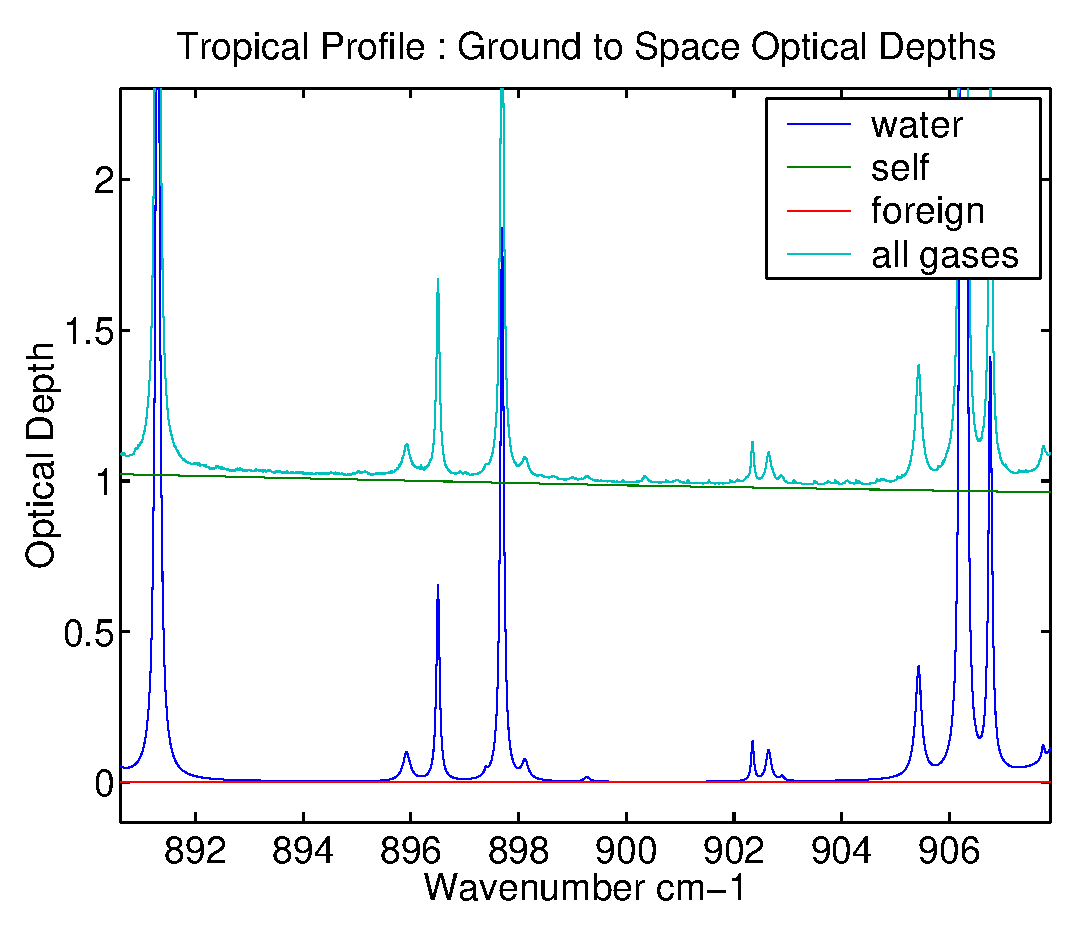
\includegraphics[width=5.5in]{FIG/water_tropical.eps}
\caption{Water and total optical depths in 10 um window.}
\label{watertrp}
\end{figure}

\begin{figure}
\includegraphics[width=5.5in]{FIG/water_subarticwinter.eps}
\caption{Water and total optical depths in 10 um window.}
\label{watersaw}
\end{figure}

Example : Suppose 3 gases have been found in $nm\_molgas$ or $nm\_xscgas$ and 
400 mixed paths defined using $nm\_weight$ and 2 atmospheres defined in
$nm\_radnce$.  The following are examples of what output paths the user can 
specify

\medskip
\medskip
\ttab iaPrinter(1) = 1\\
\ttab iaGPMPAtm(1) = 1\\
\ttab iaNp(1) = -1\\

\medskip
\noindent
will list ALL spectra for ALL gases.  For each 10000 point chunk,
the kProfLayers layers of gas 1, kProfLayers layers of gas 2 and kProfLayers 
layers of gas 3 will be output (10000 pts per layer).

\medskip
\medskip
\ttab iaPrinter(1) = 1\\
\ttab iaGPMPAtm(1) = 1\\
\ttab iaNp(1) = 2\\
\ttab iaaOp(1,1)=10\\
\ttab iaaOp(1,2)=20\\
\ttab \\
\ttab iaPrinter(2) = 1\\
\ttab iaGPMPAtm(2) = 2\\
\ttab iaNp(1) = 1\\
\ttab iaaOp(2,1)=30\\
\ttab \\
\ttab iaPrinter(3) = 1\\
\ttab iaGPMPAtm(3) = 3\\
\ttab iaNp(3) = 2\\
\ttab iaaOp(3,1)=60\\
\ttab iaaOp(3,2)=70\\

\begin{itemize}
\item will list layers 10,20  of gas ID 1
\item will list layer  30     of gas ID 2
\item will list layers 60,70  of gas ID 3
\end{itemize}
(if for instance, GAS ID 2 were not defined in MOLGAS/XSCGAS, the program 
will halt)

\medskip
\medskip
\ttab iaPrinter(1) = 1\\
\ttab iaGPMPAtm(1) = -1\\
\ttab iaNp(1) = 5\\
\ttab iaaOp(1,1)=1\\
\ttab iaaOp(1,2)=2\\
\ttab iaaOp(1,3)=3\\
\ttab iaaOp(1,4)=4\\
\ttab iaaOp(1,5)=5\\

\smallskip\noindent
will output the spectra for the 5 lowest layers for ALL gases.

\medskip
\medskip
\ttab iaPrinter(1) = 1\\
\ttab iaGPMPAtm(1) = 2\\ 
\ttab iaNp(1) = -1\

\smallskip\noindent
will output the spectra for ALL kProfLayers layers for GAS ID = 2

\medskip
Note that for options 1 these outputs can be layer to space cumulative, 
layer to space transmittances, layer or layer transmittances, depending on 
the relevant setting of parameter 1 {\sf kLayer2Sp} in $nm\_params$

\subsubsection{Output mixed paths (Option 2 : IaPrinter(iI)=2)}

\vspace{0.1in}
\noindent For this iOutputOption ( = 2), the user needs to specify iSet 
(mixed path set) and list of mixed paths to output. The program expects one 
of the following four combinations of {\sf iWhich iNp} : \\

\vspace{0.2in}
\begin{small}
\begin{longtable}{|c|c|p{\colwidth}|}
\caption{Output options for iaPrinter(iI)=2}\\
\hline
iaGPMPAtm& iaNP & DESCRIPTION\\ \hline
-1   &  -1   & all mixed paths output\\ \hline
iSet &  -1   & for mixed path set = iSet, output all kProfLayers layers\\ 
               \hline
-1   & iN    & for all mixed path sets iMP=1,iSetNum,  output spectra in 
               the iN layers specified in list on next line\\ \hline
iSet & iN    & for mixed path set iSet, output spectra in the
              iN layers specified in list on the next line\\ \hline
\end{longtable}
\end{small}
If iaNP(iI) is not equal to -1, then the next line should contain a 
list of the iaNP(iI) mixedpaths to be output

Note that iaPrinter(iI) = 2 can be repeated more than once---the 
instructions found each time it finds iaPrinter(iI) =  2 are simply merged
together with the previous instructions.  Thus for instance

\medskip
\ttab iaPrinter(1) = 2\\
\ttab iaGPMPAtm(1) = 1\\
\ttab iaNp(1)      = -1\\
\ttab iaPrinter(1) = 2\\
\ttab iaGPMPAtm(1) = 2\\
\ttab iaNp(1)      = -1\\

\medskip
\noindent
are perfectly valid, as the program will output the spectra for all
kProfLayers layers for mixed path sets 1 and 2

Example : Suppose 3 gases have been found in $nm\_molgas$ and $nm\_xscgas$ 
and 4 mixed path sets (or 400 mixed paths) defined using $nm\_weight$ and 2 
atmospheres defined in $nm\_radnce$.  The following are examples of what 
output mixed paths the user can specify.

\medskip
\medskip
\ttab iaPrinter(1) = 2\\
\ttab iaGPMPAtm(1) = -1\\
\ttab iaNp(1)      = -1\\

\medskip
\noindent
will list ALL spectra for ALL mixed path sets.  For each 10000 point chunk,
the kProfLayers layers of set 1, kProfLayers layers of set 2, kProfLayers 
layers of set 3 and kProfLayers layers of set 4 will be output 
(10000 pts per layer).

\medskip
\medskip
\ttab iaPrinter(1) = 2\\
\ttab iaGPMPAtm(1) = 1\\
\ttab iaNp(1)      = 2\\
\ttab iaaOp(1,1)   = 10\\
\ttab iaaOp(1,2)   = 20\\
\ttab \\
\ttab iaPrinter(2) = 2\\
\ttab iaGPMPAtm(2) = 2\\
\ttab iaNp(2)      = 1\\
\ttab iaaOp(2,1)   = 30\\
\ttab \\
\ttab iaPrinter(3) = 2\\
\ttab iaGPMPAtm(3) = 3\\
\ttab iaNp(3)      = 2\\
\ttab iaaOp(3,1)   = 60\\
\ttab iaaOp(3,2)   = 70\\

\begin{itemize}
\item will list layers 10,20  of MP set 1
\item will list layer  30     of MP set 2
\item will list layers 60,70  of MP set 3
\end{itemize}
(if for instance, the user tried to output something from MP set 5, the 
program will halt as this set was undefined)

\medskip
\medskip
\ttab iaPrinter(1) = 2\\
\ttab iaGPMPAtm(1) = -1\\
\ttab iaNp(1)      = 5\\
\ttab iaaOp(1,1)   = 1\\
\ttab iaaOp(1,2)   = 2\\
\ttab iaaOp(1,3)   = 3\\
\ttab iaaOp(1,4)   = 4\\
\ttab iaaOp(1,5)   = 5\\

\smallskip\noindent
will output the spectra for the 5 lowest layers for ALL four mixed path sets.

\medskip
\medskip
\ttab iaPrinter(1) = 2\\
\ttab iaGPMPAtm(1) = 2\\
\ttab iaNp(1)      = -1\\

\smallskip\noindent
will output the spectra for ALL kProfLayers layers for mixed path set number 2

\medskip
\medskip
\ttab iaPrinter(1) = 2\\
\ttab iaGPMPAtm(1) = -1\\
\ttab iaNp(1)      = -1\\

\smallskip\noindent
will list all 400 mixed path spectra

\medskip
Note that for option 2, these outputs can be layer to space cumulative, 
layer to space transmittances, layer or layer transmittances, depending on 
the relevant setting of parameter 1 {\sf kLayer2Sp} in $nm\_params$

\subsubsection{Output radiances (Option 3 : iaPrinter(iI) = 3)}

\vspace{0.1in}
\noindent For iOutputOption = 3, the user needs to specify iAtm (atmosphere 
number). For this option, the program expects one of the following 
four combinations of {\sf iaGPMPAtm iaNp} : \\
\vspace{0.2in}
\begin{small}
\begin{longtable}{|c|c|p{\colwidth}|} 
\caption{Output options for iOutputOption=3}\\
\hline
iaGPMPAtm & iaNp & DESCRIPTION\\ \hline
-1  & -1  & radiances for all layers in all atmospheres output\\ \hline
iAtm & -1  & for atmosphere iAtm, output radiances at all layers (bottom or
             top, depending on up or down looking instrument) \\ \hline
-1   & iN  & for all atmospheres, output radiances at the iN pressures    
             specified  in the next line\\ \hline
iAtm &  iN  & for atmosphere iAtm, output radiances at the iN pressures   
              specified in the next line\\ \hline
\end{longtable}
\end{small}
If iaNP(iI) is not equal to -1, then the next line should contain a 
list of the iNP pressures at which to output radiances.

As in the case of concatenating paths/mixed paths output, 
for a specific radiating atmosphere, if iOutputOption=3 is repeated 
more than once, the program tries to merge the pressures together, as long as
no more than kProfLayers different pressures found for any one of the 
individual atmospheres.  In addition , if iAtm $<$ 0, as the program keeps 
on adding each atmosphere as a new print option, the program will halt if the 
total number of print options exceeds kMaxPrint.  Thus

\medskip
\ttab iaPrinter(1) = 3\\
\ttab iaGPMPAtm(1) = 1\\
\ttab iaNp(1)      = 1\\
\ttab raaOp(1,1)   = 0.01\\
\ttab iaPrinter(1) = 3\\
\ttab iaGPMPAtm(1) = 1\\
\ttab iaNp(1)      = 1\\
\ttab raaOp(1,1)   = 0.10\\

\medskip
\noindent 
is allowed.  However if kMaxPrint=5 and there are 6 atmospheres
defined in $nm\_radnce$, then

\medskip
\ttab iaPrinter(1) = 3\\
\ttab iaGPMPAtm(1) = -1\\
\ttab iaNp(1)      = -1\\

\medskip
\noindent
will cause the program to stop.

Example : Suppose as in the above example, 3 gases have been found 
in $nm\_molgas$ and $nm\_xscgas$, 400 mixed paths defined using $nm\_weight$
and 2 atmospheres defined in $nm\_radnce$ (with the start/stop pressures 
being such that the first one has 90 layers and the other has 100 layers).  
The following are examples of what output radiances the user can specify

\medskip
\ttab iaPrinter(1) = 3\\
\ttab iaGPMPAtm(1) = -1\\
\ttab iaNp(1)      = -1\\

\medskip\noindent
will list the radiances at the top of each layer (or bottom if the radiation
traveling down to instrument on ground), for each atmosphere.  Thus there 
will be 90 radiances from atmosphere 1, and 100 from atmosphere 2

\medskip
\ttab iaPrinter(1) = 3\\
\ttab iaGPMPAtm(1) = 2\\
\ttab iaNp(1)      = -1\\

\medskip\noindent 
will list the radiances at the top of each layer (or bottom if the
radiation traveling down to instrument on ground), for atmosphere
number 2.  Thus there 100 radiances from atmosphere 2

\medskip
\ttab iaPrinter(1) = 3\\
\ttab iaGPMPAtm(1) = -1\\
\ttab iaNp(1)      = 2\\
\ttab raaOp(1,1)   = 10.0\\
\ttab raaOp(1,2)   = 0.01\\

\medskip\noindent 
will list two radiances for each atmosphere.  These radiances are
computed at pressures 10.0 and 0.01 mb (if one or both the
atmospheres does not contain these pressures, the program will halt)

\medskip
\ttab iaPrinter(1) = 3\\
\ttab iaGPMPAtm(1) = 2\\
\ttab iaNp(1)      = 3\\
\ttab raaOp(1,1)   = 700.0\\
\ttab raaOp(1,2)   = 10.0\\
\ttab raaOp(1,3)   = 0.01\\

\medskip\noindent 
will list three radiances for atmosphere 2.  These radiances are
computed at pressures 700.0, 10.0 and 0.01 mb (if the atmosphere
does not contain these pressures, the program will reset the
pressures so that they are within the max/min specified by the user
in $nm\_radnce$)

Note that the program takes into account the pressure layering, and the 
pressures where the radiance is to be output. As an example, suppose that
the top pressure layer is from 10 mb to 0.005 mb , and the aircraft carrying 
the downlooking instrument flies at 5.0 mb. For downlooking instruments, 
the program uses the $lower$ portion of the layer when doing its fractional
layering computations, except for the bottommost layer (see below). 
So in this example, only fraction rF=(10-5)/(10-0.005) ~ 1/2 = rFracTop of 
the top layer is used.

\begin{verbatim}
    --------------

    //////////////          use this LOWER portion
    --------------
\end{verbatim}

If a print option for this atmosphere is\\
\medskip
\ttab iaPrinter(1) = 3\\
\ttab iaGPMPAtm(1) = 1\\
\ttab iaNp(1)      = 1\\
\ttab raaOp(1,1)   = 00.0\\
implying that one radiance, at aircraft height, is to be output, then
the program will compute the output radiance as follows : \\
the radiance immediately below this layer is the incident radiation. A 
fraction 0.5 (=rFracTop) of the layer is to be used in the radiative transfer.
The program interpolates the vertical temperatures, to find the temperature
of this fractional layer, and then uses rFracTop of the computed absorption
coefficients, to find the absorption in this fractional layer. These
are then used, together with the radiation at the bottom of the layer, to
compute the radiance at the instrument.

If a print option for this atmosphere is\\
\medskip
\ttab iaPrinter(1) = 3\\
\ttab iaGPMPAtm(1) = 1\\
\ttab iaNp(1)      = 1\\
\ttab raaOp(1,1)   = 7.5\\
(ie the user wants a radiance output at pressure 7.5 mb), the program will 
compute the output radiance as follows : \\
the radiance immediately below this layer is the incident radiation. A 
fraction 0.25 (= (10-7)/(10-0.005)) of the layer is to be used in the 
radiative transfer.
The program interpolates the vertical temperatures, to find the temperature
of this fractional layer, and then uses rFrac of the computed absorption
coefficients, to find the absorption in this fractional layer. These
are then used, together with the radiation at the bottom of the layer, to
compute the radiance at the instrument. 

As mentioned immediately above, the program is very careful about the 
bottommost layer, and will use the $top$ fraction of this layer (between
the ground and specified pressure level). For example, if the bottom layer is 
from 1000 mb to 900 mb, and the surface pressure  is 950 mb, then only 
fraction rF=(950-900)/(1000-900) ~ 1/2 =  rFracBot of the bottom layer is used
\begin{verbatim}
    --------------
    //////////////          use this UPPER portion
    //////////////

    --------------
\end{verbatim}
If a print option for this atmosphere is \\
\medskip
\ttab iaPrinter(1) = 3\\
\ttab iaGPMPAtm(1) = 1\\
\ttab iaNp(1)      = 1\\
\ttab raaOp(1,1)   = 1000.0\\
this means that the radiation at the surface is output : \\
raRad(vu) = raEms(vu) * ttorad(Tsurf,vu) + thermal(vu) + solar(vu)

If a print option for this atmosphere is
\medskip
\ttab iaPrinter(1) = 3\\
\ttab iaGPMPAtm(1) = 1\\
\ttab iaNp(1)      = 1\\
\ttab raaOp(1,1)   = 925\\

implying that one radiance, at 925 mb, is to be output, then the fraction of 
the bottom layer that will be used is rFracBot - (925-900)/(1000-9000) = 
0.5 - 0.25 = 0.25. The program will compute the output radiance as follows : \\
the radiance from the surface is used as the incident radiation. A 
fraction 0.25 of the layer is to be used in the radiative transfer.
The program interpolates the vertical temperatures, to find the temperature
of this fractional layer, and then uses rFrac of the computed absorption
coefficients, to find the absorption in this fractional layer. These
are then used, together with the surface radiation, to compute the radiance at 
the instrument. 


If the user specifies radiances to be output at EACH layer \\
\medskip

\ttab iaPrinter(1) = 3\\
\ttab iaGPMPAtm(1) = 1\\
\ttab iaNp(1)      = -1\\

then for each layer, the radiation at uppermost part of the layer is output\\
ie bottom layer : surface to top of layer           --> output rad\\
     next layer : bottom of layer to top of layer   --> output rad \\
       ....          .......                      ...\\
      top layer : bottom of layer to aircraft posn  --> output rad \\

The same considerations would be applied for a uplooking instrument.

Note that if you use the clear sky radiative transfer code, you 
can output radiances at as many levels as you desire; however if you turn on
the scattering code, at present you can only output the radiance at the TOA 
(for downlook instrument) or at surface (for uplook instrument); if some other
option is found in the namelist, the code will stop.

Also note how if iaPrinter(iI) = 1,2 we had to specify the gas paths
or mixed paths in iaaOp(i,j), but if iaPrinter(iI) = 3 we had to specify the 
pressure levels in raaOp(i,j)

\subsection{$nm\_jacobn$ (optional)}

This keyword turns on/off Jacobian calculations.  
The user can either ask to output the first kMaxDQ gases, or give a list 
containing which gas IDs he wants to output gas amount Jacobians for, or
turn off jacobian computations :

\smallskip
\ttab {\sf iJacob = -1}

{\em OR} \\

\ttab {\sf iJacob = n}\\
\ttab {\sf g1  g2  ... gn}

{\em OR} \\
\ttab {\sf iJacob = 0}

If$iJacob = 0$, then no Jacobian computations are done. 

Depending on the setting of parameter $kJacobOutput$ in the PARAMS section,
the jacobians that are output could be the raw jacobians (dr/ds), 
the brightness temperature jacobians (d(BT)/ds) or the scaled
brightness temperature jacobians (d(BT)/ds $\times \delta$ s) where $s$ is the
variable with respect to which the jacobian is being computed (gas amount,
temperature or surface parameter) ($kJacobOutput = -1,0,1)$.

In addition, depending on the setting
of parameter  $kTempJac$ in the PARAMS section, the temperature Jacobian 
could be computed using the temperature dependence of only the planck terms, 
the transmission terms or both ($kTempJac = -2,-1,0$)

For a downlooking instrument, the code will output gas jacobians for all
gases found in the list in the JACOBN section, temperature jacobians, 
weighting functions, and four surface jacobians : the radiance change with 
respect to surface temperature, surface emissivity, thermal background and 
solar background.

For an uplooking instrument, the code will output gas jacobians for all
gases found in the list in the JACOBN section, temperature jacobians, 
weighting functions. Since surface terms are meaningless here, four sets of 
zeros are also output. 

If the user wants \kc to do scattering computations, then jacobian
computations can be done, by assuming that the cloud (or scattering volume) 
only has an abosprptive component. If the user imports spectra for some
gases from some line by line code, no jacobian computations can be done as
\kc cannot ``perturb'' the gases in temperature.

\textcolor{red}
{WARNING : \kc has been structured so that the total water optical depth is
broken into that of three components, according to the CKD definitions : 
gasID = 1 being the without basement lorentz term, gasID = 101 being the self
continuum and gasID = 102 being the foreign continuum. An unsuspecting user
might only turn gasID = 1 on, and be puzzled why the water jacobians seen
in the output files seems small (eg in the 10 um window region, the main 
contribution is due to the self continuum). Thus the user should ask for gases
1,101 and 102 to be output!!!!}

\subsection{$nm\_nonlte$ (optional)}
The default behaviour of \kc is to assume the entire atmosphere is in local
thermodynamic equilibrium. This assumption is used in compiling the kCompressed
Database using our UMBC-LBL code. However, AIRS observations, and indeed 
observations by many limb viewers, indicate that some molecules are not in LTE
in the upper layers of the atmosphere. In particular, the 4 um band of CO2 is
significantly in NonLTE above 60 km, during daytime. 

To account for this, we have implemented a NonLTE capability into \kc, 
optimized and tested for the 4 um CO2 bands. However, since the line shapes 
and planck function modifiers need to be computed on the fly, for the many CO2 
lines in this region of the spectrum, the code is significantly slowed down!!!

In addition, to simplify the computations, we mainly use Cousin chi functions 
instead of line mixing in this region. However, for the R branch of the strong
$\Sigma-\Sigma$ band, in the important temperature sounding region (2380 to 
2430 \wn), the code does a first order linemixing times an appropriate ``chi''
function. This should not really affect the results too much, as NLTE is in
the higher parts of the atmosphere (stratopause), mininising the effects of 
linemixing and thereby rendering the Cousin lineshape as ``good enough.'' In 
the lower part of the atmosphere (tropopause), pressures are high enough to 
warrant a linemixing lineshape; in this region the atmosphere is in LTE, and
\kc essentially uses its default (linemix) database here.

The code works as follows. It first uncompresses the optical depths for all 
layers, for the gas in question (ie it assumes all layers are in LTE). It 
then does a LBL computation for the upper layers of the atmosphere, using 
parameters and data supplied below.

The information required in this section is of the following form\\
\medskip
\ttab iNumNLTEGases             = \\
\ttab iNLTE\_SlowORFast          = \\
\ttab iaNLTEGasID(1..N)         = \\
\ttab raLTEStrength(1..N)       = \\
\ttab raNLTEstart(1..N)         = \\
\ttab iaNLTEChunks(1..M)        = \\
\ttab iaaNLTEChunks(1..N,1..M)  = \\
\ttab caaStrongLines(1..N)      = \\
\ttab caaUpperMixRatio(1..N)    = \\
\ttab caWeakCO2Path             = \\
\ttab iaNLTEBands(1..N)         = \\
\ttab caaNLTETemp(1..N)         = \\
\ttab caaNLTEBands(1..N,1..P)   = \\
\ttab

\noindent $iNLTE_SlowORFast$ tells the code whether to use the slow accurate
LBL model (+1) or regression coefficients used by the fast model (-1). If you
use the Fast Version (+1), then the only namelist parameters you need to 
set are iNumNLTEGases,iNLTE\_SlowORFast,iaNLTEGasID(),iaNLTEChunks(a),
                  iaaNLTEChunks(a,b)

\noindent $iNumNLTEGases$ tells the code the number of gases that are in NLTE.
If NLTEGases = -1, then all gases are in LTE (no gas in NLTE). The code uses 
the defualt kCompressed Database for $all$ gases.

If NLTEGases > 0, then one or more gases are in NLTE; all other gases are in 
LTE, and the code uses the default kCompressed Database for these gases; for 
the $N$ gases that are in NLTE, the code will perform line by line computations
based on information specified further in this section.

\noindent $iaNLTEGasID(1..N)$ gives the HITRAN gas IDs of the $N$ gases in NLTE

\noindent $iSetBloat$ tells code whether to use default (-1) 0.0025 \wn 
spacing or to use bloted (+1) 0.0005 \wn resolution.\\
If iNLTE\_SlowORFast = +1, this is automatically (re)set to -1

\noindent $iDoUpperAtmNLTE$ tells code whether to do NLTE calcs upto 80 km 
(default (-1) or upto 120 km (+1)\\
If iNLTE\_SlowORFast = +1, this is automatically (re)set to -1

\noindent $raNLTEstart(1..N)$ tells for each gas in NLTE, at which height 
(in km) to start the NLTE computations. This height information is turned into
the relevant layer; for all layers below this, the code 
uses the optical depths from the kCompressed Database.

\noindent $raLTEStrength(1..N)$ is akin to the ``weight'' section; this tells 
the code the multiplier for the spectral computations performed by the code.
Obviously this parameter will usually be 1.0 for almost all cases.\\
\textcolor{red}
{You can be very mischievous and use a different database for CO2 here!!!!! \\
If gasID == 2, raLTEStrength(X) < 0 then kCARTA will go ahead and say, aha, 
you do not want NLTE but you simply want to substitute the LINEMIX compressed
database optical depths for eg COUSIN compressed database optical depths. So
\kc will simply substitute the optical depths of the upper layers with 
data from \emph{kCousin\_CO2Path}. So if you cleverly set the value of 
raNonLTEStart(X) = -1400, then $all$ layers will be substituted, not just the 
upper layers!!!!! Devilish, eh?. A nice parameter to use for raLTEStrength(X)
in this case is -1.1212, which is 370/330 ppmv used in the newer linemix
database vs that used in the older Cousin database}

\noindent $iaNLTEChunks(1..N)$ tells for which chunks the above gases are in 
NLTE

\noindent $iaaNLTEChunks(1..N,1..M)$ for each of the $N$ gases in NLTE, we now 
know how many chunks are in NLTE. iaaNLTEChunks specifies these chunks.

%caa_UA_LTEWeakBack_StdOptDepth is no longer used
%\noindent $caa_UA_LTEWeakBack_StdOptDepth(1..N)$ for each of the $N$ gases in 
%NLTE, we now know how many chunks are in NLTE. The spectroscopy says there are
%strong bands, and weak background lines. caa\_UA\_LTEWeakBack\_StdOptDepth 
%tells the code where to find the optical depths of the weak background lines, 
%computed for a US Standard Atmosphere in LTE, ABOVE 0.005 mb (80 km) height.
%\textcolor{blue}
%{NOTE THAT THIS HAS NOT YET BEEN COMPUTED FOR THE UA, using UMBC-LBL. In other
%words, we look at a database that has been computed from 1200 - 0.005 mb, 
%and say, hah, let's just use this database above 0.005 mb, as right now we are
%not debugging the extension of kCARTA to work above 0.005 mb }
%\textcolor{red}
%{All the weak background lineshapes are just plain old Voigt functions; they
%are computed for the US Standard profile, but since they are the weak lines, 
%and since the $kLAYERS$ code pads the upper atm with the US Standard profile
%in any case, this should NOT be too bad an assumption. The code does adjust
%the optical depths to the actual gas profile amounts in the layers.}

\noindent $caaUpperMixRatio(1..N)$ tells the code where the stratosphere/ 
mesosphere mixing ratios can be found. Remember the default kCARTA
database extends from 0 to 80 km, while NLTE is important between about
40-120 km; so kCARTA can compute optical depths and Planck modifiers above
the standard database, as long as it knows the ppmvs!
\textcolor{red}
{Right now it scales the MR read in from this file, to 370 ppmv at bottom}

\noindent $caaStrongLines(1..N)$ for each of the $N$ gases in NLTE, we now 
know how many chunks are in NLTE. The gas molecules have many lines/bands; 
from $caWeakCO2Path$ there are the weak background lines, and also there are
strong lines in bands. Some bands are in LTE while others are in NLTE. 
caaStrongLines is a file that specifies all the bands for the ``strong'' 
lines \textcolor{red}{that could be in LTE or NLTE}. Depending on what bands
are specified to be in NLTE in $caaaNLTEBands(1..N,1..P)$, an $XOR$ is done
with the bands in $caaStrongLines$ to compute the optical depth contribution
due to strong bands in LTE (the NLTE lines will have their optical depths 
computed separately). 
\textcolor{red}{The files listed in this MUST have the FULL path and name} \\
\textcolor{blue}{The files listed must agree with those listed by 
                appending $caStrongLineParams$ in the ``NLTEBandMapper'' 
                subroutine, else the code gets very perplexed}

\noindent $iaNLTEBands(1..N)$ tells for each gas, how many bands are in NLTE

\noindent $caaaNLTEBands(1..N,1..P)$ for each of the $N$ gases in NLTE, give
the igasID,iISO,iUSGQ numbers so that kCARTA maps these partams to a file
that has the weak HITRAN line parameters (such as line centers, 
broadening coefficients etc).
\textcolor{red}
{The lineshapes for these strong lines will be Voigt * Cousin if the gas is 
CO2; else they will just be Voigt}

\noindent $caaNLTETemp(1..N)$ for each of the $N$ gases in NLTE, give
the file that has the NONLTE temperatures and vibrational partition function 
terms, in GENLN2 style. 
If the user puts the name 'nlteguess', kCARTA will use a polynomial guess
of the NLTE temps, and output the guessed profile into \\
   caOutName\_VTX     : this is the GENLN2 style file \\
   caOutName\_VTX.sss : this is a summary of the GENLN2 style file \\
where ``X'' is the closet regression profile (of 48) to the user profile, 
between 800 and 25n mb (2 - 25 km). The .sss file will have 15 columns : \\
   ii,P,Tk,[QV1,QV2,QV3,QV4],[S1,S2,S3,S4],[P1,P2],[D1,D2] \\
where the $QV{i},i=1,4$ are the vib partition functions, the SSi,PPi,DDi are 
the isotopic sigmasigma, pipi, deltadelta NLTEs.

The example below is primed for the 4 um CO2 band. \\
\begin{itemize}
\item iNumNLTEGases = +1 : says that one gas is in NLTE
\item iNLTE\_SlowORFast = +1 : says that slow accurate LBL model
\item  iaNLTEGasID(1)    = 2 : says the gasID of the gas is ``2'' (CO2)
\item  raNLTEstrength(1) = +1.0 : says use a weight of 1.0 for all the
                          upper layer optical depths computed for this gas
\item  raNLTEstart(1)   =  45.0 : tells the code to start the NLTE 
                     computations above 45.0 km (which is about layer 90 for 
                     the standard AIRS layers)
\item iaNLTEChunks(1) = 10 : says that 10 chunks are in NLTE
\item iaaNLTEChunks(1,1..10) gives the 10 chunks that are in NLTE
\item caaLTEWeakLines(1) gives the file that has the parameters for the
            weak lines that are in LTE.
\item iaNLTEBands(1) = 8 : says that for this gas, there are 8 bands in NLTE
\item caaaNLTEBands(1,1..8) are strings that give the (iGasID iISO iLSGQ iUSGQ)
      numbers so kCARTA finds the names of the files that contain the
      HITRAN lineparameters of the vibrational bands in NLTE. Any other info
      in the string is ignored; the info is then mapped onto UMBC-LBL 
      identifiers so that kCARTA can open the correct files containing the 
      line paameters for the band in question. At present only CO2 4um bands
      can be included.
\item caaNLTETemp(1) gives the names of the file that contains the
       NLTE profiles, as well as the vibrational partition functions, in GENLN2
       style.
\end{itemize}

\vspace{0.25in} 
Following is a typical NLTE identifier section for the 4.3 um CO2 region. Note
how we identify the sigma-sigma, pi-pi and delta-delta lines.

\begin{verbatim}
 iNumNLTEGases    =             +1 
 iNLTE_SlowORFast =             +1 
 
 iaNLTEGasID(1)      =        2 
 raNLTEstrength(1)   =        +1.0 
 raNLTEstart(1)      =        45.0
 iaNLTEChunks(1)       =        10 
 caaNLTETemp(1)  = '/home/sergio/AIRSCO2/NONLTE/hit2350_day_profile3A'  
 caaLTEWeakLines(1) ='/home/sergio/AIRSCO2/NONLTE/CO2/co2_2230.dat' 

 iaaNLTEChunks(1,1)  =         2230 
 iaaNLTEChunks(1,2)  =         2255 
 iaaNLTEChunks(1,3)  =         2280 
 iaaNLTEChunks(1,4)  =         2305 
 iaaNLTEChunks(1,5)  =         2330 
 iaaNLTEChunks(1,6)  =         2355 
 iaaNLTEChunks(1,7)  =         2380 
 iaaNLTEChunks(1,8)  =         2405 
 iaaNLTEChunks(1,9)  =         2430 
 iaaNLTEChunks(1,10) =         2455 
 
 iaNLTEBands(1)     = 19
 !!! uses strongest  sigma-sigma, pi-pi, delta-delta 
 !!! 2350 .. 2354 = sigma-sigma 
 !!! 2320 .. 2322 = pi-pi 
 !!! 2310 .. 2312 = delta-delta 
 !!!                 GASID   GASIso  iLSGQ     iUSGQ   run7lblID 
 caaaNLTEBands(1,1) ='2        1       1         9        2350' 
 caaaNLTEBands(1,2) ='2        2       1         9        2351' 
 caaaNLTEBands(1,3) ='2        3       1         9        2352' 
 caaaNLTEBands(1,4) ='2        4       1         9        2355' 
 caaaNLTEBands(1,5) ='2        1       2         16       2320' 
 caaaNLTEBands(1,6) ='2        2       2         16       2321' 
 caaaNLTEBands(1,7) ='2        1       4         24       2310' 
 caaaNLTEBands(1,8) ='2        2       4         24       2311' 
 caaaNLTEBands(1,9) ='2        1       3         23       2353'  
 caaaNLTEBands(1,10)='2        1       5         25       2354'  
 !!!these are the ones Manuel suggested adding on; some isotopes of above
 caaaNLTEBands(1,11)='2        2       3         23       2253'  
 caaaNLTEBands(1,12)='2        2       5         25       2254'  
 !!!these are the others Manuel suggested adding on
 caaaNLTEBands(1,13)='2        1       2         15       2110'  
 caaaNLTEBands(1,14)='2        1       3         25       2120'  
 caaaNLTEBands(1,15)='2        1       5         23       2140'  
 caaaNLTEBands(1,16)='2        1       6         36       2160'  
 caaaNLTEBands(1,17)='2        1       7         37       2170'  
 caaaNLTEBands(1,18)='2        1       8         38       2180'  
 caaaNLTEBands(1,19)='2        3       2         16       2322'
 !!!these one never seems to exist in the NLTE profiles
 caaaNLTEBands(1,20)='2        1       3         22       2150'  
 caaaNLTEBands(1,21)='2        1       4         22       2130'  
 $end 

\end{verbatim}

In addition, \kc can output a file containing the Planck modifiers. This file 
is in the same output format as the flux file. Control for turning this 
on/off is thru parameter kFlux in $nm\_param$; set to -1,1,2,3 (off) or 0 (on)

Figure ~\ref{nlte} shows a comparison plot of kCARTA vs GENLN, compared to some
actual NLTE data seen in daylight viewing conditions on the AIRS instrument.
What is plotted for AIRS, is actual NLTE dayime observations minus LTE Fast 
Model computations. For KCARTA and GENLN2, we plot (NLTE - LTE) calculations,
with the TOA at about 85 km. The main CO2 Sigma-Sigma, Delta-Delta, Pi-Pi 
bands are in NLTE while the weak background lines are in LTE. 

\begin{figure}
\includegraphics[width=5.5in]{FIG/nlte.eps}
\caption{NLTE plots : Comparison of kCARTA, GENLN to actual AIRS data.}
\label{nlte}
\end{figure}

\subsection{$nm\_scattr$ (optional)}

If $kRTP = -2,-1,0$ this means the user will be defining the atmosphere and
any scattering parameters, using the specifications stated below. If 
$kRTP = +1$ then \kc will use the atmosphere and cloud definitions specified 
in the RTP file that contains the profile; the documentation can be found in 
KLAYERS/Src/Doc. 

This keyword turns on/off scattering calculations.  \kc can interface with 
one of five scattering codes, depending on the users needs. 

The first is $rtspec.f$ written by K. F. Evans of the University of Colorado 
at Boulder. This code computes the scattering using one of three  models : 
Single Scattering(1), Eddington(2) or a Hybrid(3) combination of the 
first two. This code is very fast, but it does not allow the user to include
scattering by a beam.

The second is $disort.f$ written by K. Stamnes $et. al.$ To speed up the 
running of this part
of the code, \kc allows the user to compute the scattering using one of three 
ways. These ways essentially allow the user to compute radiative transfer on 
$N$ out of the 10000 points per chunk and then interpolate onto the rest of 
the wavenumber grid. The three ways differ in the way they choose the 
wavenumber points to do the radiative transfer on. This code is slow, but 
it does allow the user to include scattering by a beam.

The third is a twostream code that also allows for the inclusion of a solar 
beam. This code has been developed here at UMBC, and is very fast.

The fourth is a languishing code (perturbative solution to Schwatzchild) and
will be implemented once Mathematica can figure out the required integrals.
(it WILL work, bloody hell!!!)

The fifth code also allows for the inclusion of a solar beam. This code is 
based on the longwave parametrizations and is also very fast, and transperant
enough to allow for jacobians to be computed.

\subsubsection{kRTP = -2,-1,0}
The user has to tell the code which of the above five scattering models 
$kWhichScatterCode$ to use (1 = $TWOSTREAM$, 2 = $RTSPEC$, 3 = $DISORT$, 
4 = $SIMPLE$, 5 = $PCLSAM$). 
If the user chooses $RTSPEC$ or $DISORT$, then he/she has to state which 
specific submodel $kScatter$ to use (eg for $RTSPEC$, use Hybrid or 
Eddington, for $DISORT$, use frequency or optical depth interpolation). The 
user also has to state how many clouds $iNumClouds$ are 
being  defined, and then has to define the clouds. In addition, the user has 
to indicate in which atmosphere a cloud should be used. If the user expects 
Jacobians to be computed, the radiative transfer code uses the specified
model ($TWOSTREAM,RTSPEC,DISORT,SIMPLE,PCLSAM$), but always uses the 
$PCLSAM$ model to compute jacobians.

For the code to interface to any of the scattewring codes, the user $has$ 
to set the number of clouds in this section to a value greater than zero.
If $iNclouds$ is less than 1, the code will not do a scattering computation. 

Note that a cloud has to be built up so that it occupies adjacent pressure 
layers eg it can occupy layers 12,13,14 but not 12,14,15. Also, the cloud 
must occupy full layers.

Clouds that occupy completely different heights can be processed. For example
if cloud 1 is an aerosol cloud layer from KCARTA layers 4-5, and cloud 2 is a  
cirrus cloud from kCARTA layers 43-46, $TWOSTREAM$ and $RTSPEC$ handle this by 
setting a  ``third'' cloud from layers 6-42, with IWP=0.0. $DISORT$ would 
simply just use the original two clouds, as widely separated as they are.

The information required in this section is of the following form\\
\medskip
\ttab kWhichScatterCode    = \\
\ttab kScatter             = \\
\ttab kDis\_Pts            = \\
\ttab kDis\_nstr           = \\
\ttab iScatBinaryFile      = \\
\ttab iNClouds           = \\
\ttab \\
\ttab Cloud 1 definitions \\
\ttab Cloud 2 definitions \\
\ttab ...\\
\ttab Cloud N definitions \\
\ttab

\noindent $kWhichScatterCode$ = +5 for PCLSAM, +4 for SIMPLE, +3 for DISORT, 
+2 for RTSPEC,  +1 for $TWOSTREAM$. Note that all but DISORT run very fast, 
but RTSPEC does NOT allow a solar beam.
\vspace{0.25in} 

\begin{itemize}
\item If $kWhichScatterCode$ = +1, (use $TWOSTREAM$) then $kSCatter$ tells 
the code how many times to run the radiance thru the cloud, to get better 
values for the incident radiation at cloud top and bottom, and hence better 
guesses at radiation exiting cloud top and bottom. This parameter should be 
set between 1 and 3.
\textcolor{red}
{After doing quite a few tests, the best setting of parameter $kScatter$, when 
$TWOSTREAM$ is used, is 1}

\item If $kWhichScatterCode$ = +2, (use $RTSPEC$) then  $kScatter$ = -1 
if the Single Scattering model is to be used, 2 if the Eddington model is to 
be used, or 3 if the hybrid model should be used. {\em It is best to use the 
Hybrid model when using $RTSPEC$}
\textcolor{red}
{After doing quite a few tests, the best setting of parameter $kScatter$, when 
$RTSPEC$ is used, is 3}

\item If $kWhichScatterCode$ = +3, (use $DISORT$) then everything defaults to 
$kScatter$ = +1 for now, as this seems the best option for both uplooking and 
downlooking instruments
\textcolor{red}
{After doing quite a few tests, the best setting of parameter $kScatter$, when 
$DISORT$ is used, is 1}
\end{itemize}

\noindent If $kWhichScatterCode$ = +3, (use $DISORT$) then 
\begin{itemize}
\item Everything defaults to $kScatter$ = +1 for now, as this seems the best
option for both uplooking and downlooking instruments
\textcolor{red}
{After doing quite a few tests, the best setting of parameter $kScatter$, when 
$DISORT$ is used, is 1}

\item $kScatter$ = +1 means use only kDis\_Pts pts (equally spaced over the 
kMaxPts) to do radiative transfer, and then interpolate in wavenumber to 
estimate the intensities for the rest of the wavenumber grid.  {\em It is 
best to use this model for either an up or down look instrument.} \\

If the instrument is uplooking, then a simple straightforward interpolation
of the radiance at the chosen wavenumber points, to the entire grid, is done.\\

If the instrument is downlooking, then a more elaborate computation is done. 
First the nonscattering radiative transfer is performed at all points on 
the wavenumber grid. The output radiance is then the nonscattered radiance, 
plus an interpolation of scattered radiance onto the required point. 
Let $raW$,$raNS$ be the entire $kMaxpts=10000$ wavenumber grid, and associated
clear sky radiances. Similarly, let $raX,raY$ be the wavenumber points at which
DISORT was called, along with the computed scattered radiance. Then the 
correct radiance raI(iF) at wavenumber point raW(i) is estimated to be
\[
raI(i) = raNS(i) + \delta I
\]
where $\delta I$ is an interpolation in Temperature space, then converted 
back to a radiance. In other words, for point raW(iF), find which wavenumber
points in raX bisect this  $W0 \le raW(iF) \le W1$. Find the DISORT and clear 
sky radiances at these bisecting points, and compute the temperature
differences between scattered and non scattered radiances, at these two points
\[
T0 = ttorad(W0,ScatterRad(W0)) -  ttorad(W0,NonScatterRad(W0)) 
\]
\[
T1 = ttorad(W1,ScatterRad(W1)) -  ttorad(W1,NonScatterRad(W1))
\]
Then interpolate to find the estimated correction to the non scattering 
temperature
\[
\delta T = \frac{T1-T0}{W1-W0} \times (raW(iF) - W0) + T0
\]
Add on the non scattering temperature, and change this to a radiance
\[
T_{scatter} = ttorad(raW(iF),NonScatterRad(raW(iF))) + \delta T
\]
\[
I_{estimate} = radtot(raW(iF),T_{scatter})
\]
By doing the interpolations in temperature, we can account for the variation
of Planck radiance with wavenumber (which should then have the spectral line 
dependancies in it).

\item $kDis\_Pts$ is the number of points tha \kc will compute the radiances 
at, out of the 10000 points per chunk. So if this variable is set at eg 25,
then \kc will ask $DISORT$ to compute the radiance only at 25 points, and then
interpolate the results onto the remaining 9975. This obvioulsy sppeds up 
the code, but the user has to be careful! A low setting, such as 25, for a 
downlook instrument is fine. But things get quite bad for the same setting
for an uplook instrument; a setting of 500 might be needed (but this of course
means that the code runs much more slowly!)

\item $kScatter$ = +2 means step thru kDis\_Pts pts that are chosen in the 
following way. Find the optical depths for the layer closest to ground, and 
sort them from smallest to largest. Choose the kDis\_Pts points that have the 
smallest optical depths. Do radiative transfer on these points, and then 
interpolate in optical depth to estimate the intensities for the rest of the 
wavenumber grid. 

\item $kScatter$ = +3 means step thru kDis\_Pts pts that are chosen in the 
following way. Find the optical depths for the layer closest to ground, and 
sort them from smallest to largest. Choose the kDis\_Pts points that span 
this, equally spaced from smallest to largest optical depth. (This should not
be confused with a $correlated$ $k$ method, since we do not do radiative 
transfer on multiple correlated k distributions as the vertical structure of 
the atmosphere changes). Do radiative transfer on these points, and then 
interpolate in optical depth to estimate the intensities for the rest of 
the wavenumber grid. 

\item If $kScatter = 2,3$ then for an uplook instrument, there is simply an
interpolation of scattered radiance in wavenumber space. In other words, the
scattered radiance is computed at discrete wavenumbers, {\em that are chosen
because of their ordering in lowest layer optical depths}. For the rest
of the points in the grid, just do a simple interpolation of the
scattered computations at these chosen optical depths, onto all the optical
depths (and hence all wavenumbers) found at the lowest layer. This method works
very well for an uplook instrument, as most of the radiance measured by
the instrument depends on the layer closest to the instrument.

\item For a downlook instrument, there is a more 
elaborate computation done, exactly along the lines of that for a wavenumber
interpolation for the downlooking case described earlier. However, since the
wavenumber dependence of the Planck function is quite crucial, the code 
proceeds as follows. First it chooses the wavenumber points according to the
sorted optical depths of the lowest layer, as described above. It then does the
$DISORT$ radiative transfer on the chosen points, and then non scattering
radiative transfer on all points. To interpolate the chosen points onto the
wavenumber grid, it resorts the chosen points according to wavenumber, and 
interpolates these few points onto the entire wavenumber grid, as described
above for $kScatter = 1$. However, since the wavenumbers chosen for the 
downlooking $kScatter = 2,3$ cases do not necessarily sample the 
$25 cm^{-1}$ chunk adequately in wavenumber, there are noticeable errors when 
compared to $RTSPEC$ or to $kScatter = 1$

\end{itemize}
\vspace{0.25in} 

\noindent If $kWhichScatterCode$ = +3, then  $kDis\_nstr$ tells how many 
streams should be used by DISORT (2,4,8,16 ...)
\vspace{0.25in} 

\noindent If $kWhichScatterCode$ = +3, then  $kDis\_Pts$ is used as 
described above.
\vspace{0.25in} 

\noindent $iScatBinaryFile$ = 1 if the scattering tables produced by 
$sscatmie.f$ have been translated to binary format, else it should be set 
to -1 if they are still in the original text file format.
\vspace{0.25in} 

\noindent $iNClouds$ is the number of clouds which are defined in this 
section, to be be used with the $rtspec$ code. If this number is less than 
one, than only clear sky computations will be done.
\vspace{0.25in} 

\noindent Each of the the clouds are defined and used as follows \\

\smallskip\noindent

\ttab raExp(iI) = rE \\
\ttab iaCloudNumLayers(iI) = iLayers\\
\ttab raaPCloudTop(iI,iJ) = rPTop \\
\ttab raaPCloudBot(iI,iJ) = rPBot \\
\ttab raaaCloudParams(iI,iJ,1) = IWP\\
\ttab raaaCloudParams(iI,iJ,2) = dme = mean particle size\\
\ttab iaaScatTable(iI,iJ) = iTable\\
\ttab caaaScatTable(iI,iJ) = Mie\_FileName\\
\ttab caaCloudName(iI) \ \\
\ttab iaCloudNumAtm(iI) = iNatms\\
\ttab \indent  iaaCloudWhichAtm(iI,iJ)\\

\medskip

The first line indicates how the IWPs will be scaled. If the cloud is 
``expanded'' to occupy pressure layers spanning $rPTop$ to $rPBot$, then the 
IWPs can either be the same in each of the layers (rE $\le$ 0), or they can
exponentially decrease from bottom to top as
\[
                rIWP = rIWP0 \times exp^{(-rE*(rPBot-rP)/(rPBot-rPTop))}
\]
where $rIWP0$ is the IWP specified by the user, and $rP$ is the pressure of the
current layer.

The second line gives the (integer) number of pressure layers $iLayers$ the 
cloud will occupy. These pressure layers $must$ correspond to the layers 
defined by the pressure levels from $klayers.x$.

In the next few lines, the user then has to define, for each of 
the layers, the cloud parameters; starting from the lowest pressure 
(highest layer), the user has to enter : \\
rPTop, rPBot  : real variables defining the cloud layer top, bottom pressure\\
IWP  : real parameter IWP/LWP in $g/m^{2}$\\
dme  : real parameter mean particle diameter (um)\\
iTable : integer giving scattering table number (integer)\\
Mie\_FileName : character array gives the Mie Scattering table file name\\

The user can then baptise the cloud with a name (in a character array). 
Finally the user has to tell the code in which atmosphere(s) to use the 
defined cloud. This is done in the next two lines : \\
iaNatms : integer that tells how many atmospheres the cloud has to be used\\
iaaCloudWhichAtm : integers listing these atmospheres\\

Note that the code automatically expands a cloud layers into multilayers 
spreading across the specified pressure levels eg if a user specifies a 
``one layer cloud'' from 250 to 200 mb, then kCARTA will expand this so that 
the start (top) layer is at 200 mb, and the stop (bottom) layer is 250 mb.

So for instance the following lines define a cloud that occupies three pressure
layers, and will be used in two atmospheres \\

\smallskip\noindent
\ttab kScatter         =           2\\
\ttab iScatBinaryFile  =           1\\
\ttab iNclouds         =           1\\
\ttab iaCloudNumLayers(1)    =     3\\
\ttab \\
\ttab \ttab   raExp(1) =  0.0\\
\ttab \ttab   raaPCloudTop(1,1) =  2.0000000E+02\\
\ttab \ttab   raaPCloudBot(1,1) =  2.5000000E+02\\
\ttab \ttab   raaaCloudParams(1,1,1)       = 5.0  \\
\ttab \ttab   raaaCloudParams(1,1,2)       = 20.0  \\
\ttab \ttab   iaaScatTable(1,1)    =  1\\
\ttab \ttab   caaaScatTable(1,1)   =  'cir1'\\
\ttab \\
\ttab \ttab   raExp(2) =  0.0\\
\ttab \ttab   raaPCloudTop(1,2) =  2.5000000E+02 \\
\ttab \ttab   raaPCloudBot(1,2) =  3.0000000E+02\\
\ttab \ttab   raaaCloudParams(1,2,1)       = 8.0  \\
\ttab \ttab   raaaCloudParams(1,2,2)       = 30.0  \\
\ttab \ttab   iaaScatTable(1,2)    =  2 \\
\ttab \ttab   caaaScatTable(1,2)   =  'cir2'\\
\ttab \\
\ttab \ttab   raExp(3) =  0.0\\
\ttab \ttab   raaPCloudTop(1,3) =  3.0000000E+02 \\
\ttab \ttab   raaPCloudBot(1,3) =  3.5000000E+02 \\
\ttab \ttab   raaaCloudParams(1,3,1)       = 10.0 \\
\ttab \ttab   raaaCloudParams(1,3,2)       = 40.0 \\ 
\ttab \ttab   iaaScatTable(1,3)    =  3 \\
\ttab \ttab   caaaScatTable(1,3)   =  'cir3' \\
\ttab \\
\ttab caaCloudName   =  'HappyLittleCloud' \\
\ttab iaCloudNumAtm  =             2       \\
\ttab iaaCloudWhichAtm       =     1, 2   \\

The code automatically compares the cloud top and bottom pressures against the
start/stop pressures of the atmospheres in RADNCE; if discrepancies are found,
the code will stop running.

\textcolor{red} 
{WARNING 1 : If one uses DISORT for a down looking instrument, with solar
on, then DISORT automatically uses a solar reflectance = albedo/$\pi$ (which is
the same as that used for the reflected thermal). \\
However, with nonscattering kCARTA, one can specify the solar reflectance, 
using parameter cakSolarRefl(i).
If this is set to -1, then the results for nonscattering kCARTA and cloudless
DISORT should be the same. If this is set to a non zero positive number, then
the results for nonscattering kCARTA and cloudless DISORT will be different.}

\textcolor{blue}
{WARNING 2 : At present, both DISORT and RTSPEC can only output a 
radiance at TOA or aircraft posn (for a down look instr), or at ground level 
(for a uplook instrument).}

\textcolor{red}
{WARNING 3 : DISORT is extensively tested by its authors (Stamnes et al). 
However, it runs much slower than non scatter kCARTA or RTSPEC. Instead of
computing radiative transfer at all points, kCARTA skips thru its wavenumber
points, and then interpolates the results back onto the 0.0025 $cm^{-1}$ 
grid.\\
For a 10000 point chunk, typical timings are 30 sec for kCARTA nonscatter 
(both up and downlook)m 35-40 sec for RTSPEC (up and downlook). For DISORT,
with kDis\_Pts = 200, for a downlook instrument, sun on, takes about 
240 secs, while for an uplook instrument, sun on, takes about 1200 secs).\\
To speed up the code, the user can do one or both of the following. In the 
input namelist file, one can reduce the number of streams used in the 
computation (kDis\_nstr, preset to 16), or decrease the number of points at 
which radiances are computed (kDis\_Pts, preset at 5).}

\textcolor{blue}
{WARNING 4: For a downlook instrument, iakThermal(i) is only relevant 
for RTSPEC (ie this parameter turns it off or on). DISORT will always compute
the background thermal.}

\textcolor{red}
{WARNING 5: For a downlook instrument, iakThermal(i) should be turned off when
TWOSTREAM is used, for better comparisons to DISORT}

Figure ~\ref{rtspec_down} is a plot of the brightness temperatures for 4 
cases, using the RTSPEC code (sun off). The instrument is downlooking. Case 1 
is clear sky, case 2 is cirrus cloud at 10 km, third is water cloud at 1 km
and fourth is aersol dust at ground. Mean particle sizes of 10 um were used 
for all three scattering cases,  while the particle concentrations were
1.0,1.0,10.0 g/m2 respectively.
\begin{figure}
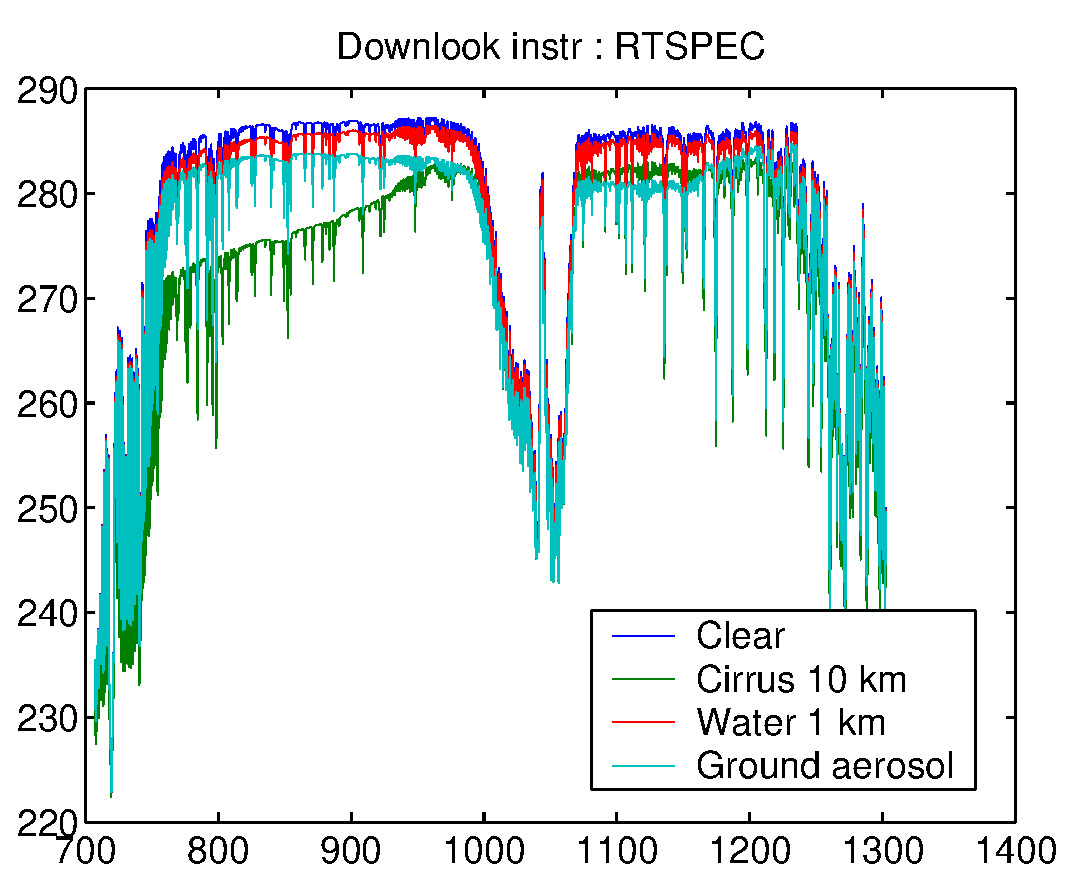
\includegraphics[width=4in]{FIG/down_rtspec.eps}
\caption{Scatter plots : Downlook instrument using RTSPEC}
\label{rtspec_down}
\end{figure}

Figure ~\ref{twostream_up} is a plot of the brightness temperatures for the 
same 4 cases, using the TWOSTREAM code (sun on). The instrument is uplooking. 
\begin{figure}
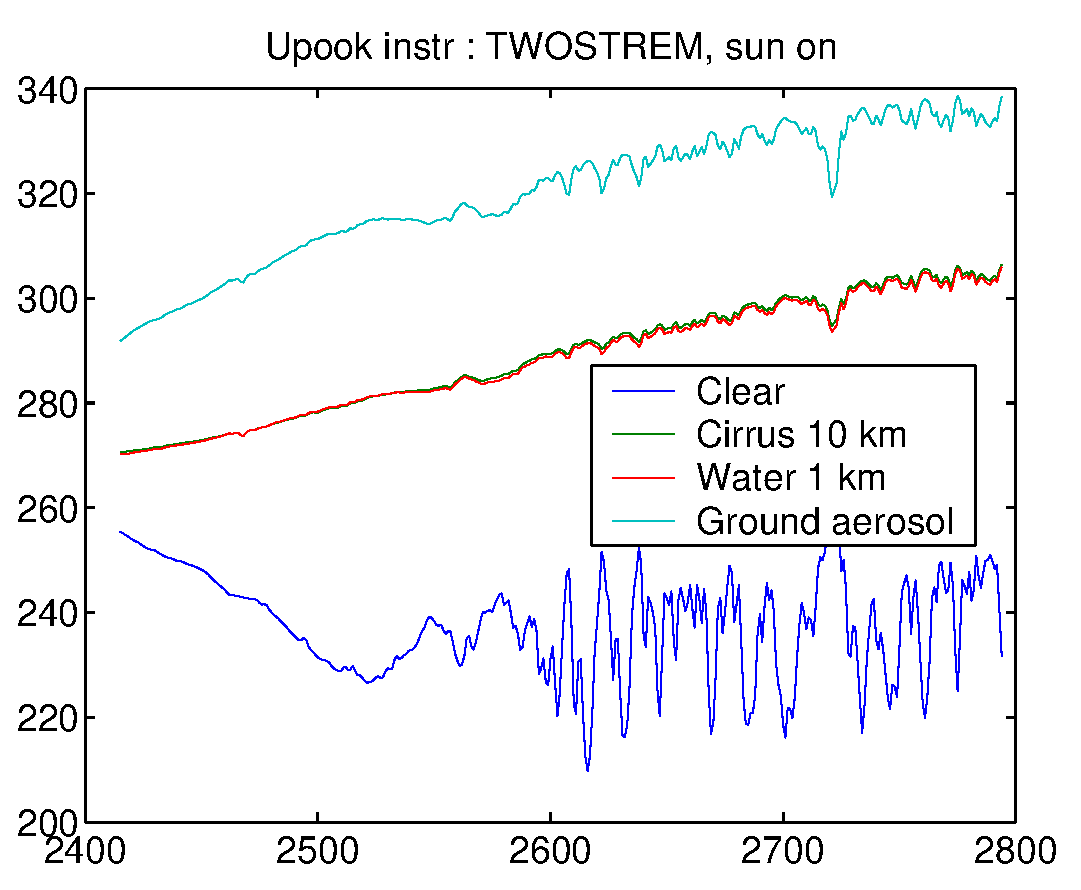
\includegraphics[width=4in]{FIG/up_two.eps}
\caption{Scatter plots : Uplook instrument using TWOSTREAM}
\label{twostream_up}
\end{figure}

\subsubsection{kRTP = +1}
Since the $AIRS$ Fast Forward Model uses a one layer version of our twostream
code, this model is automatically selected when the $RTP$ file contains 
information to include a cloud in the atmosphere. Many of the variables needed
above are then automatically set by \kc; only the very needed information
is read in from the $RTP$ file. Only $ONE$ cloud can be read in and used from 
the $RTP$ file.
\begin{verbatim}
     a) kWhichScatterCode      = +1       !use TwoStream 
     b) kScatter               = 1        !use one run of TwoStream 
     c) raExp(1)               = 0.0 
     d) iScatBinaryFile        = cbinORasc     --> set in nm\_prfile
     e) iNClouds               = 1 
     f) iaCloudNumLayers(1)    = 1 
     g) iaaScatTable(1,1)      = 1 
     h) caaCloudName(1)        = 'RTP cloud' 
     i) caaaScatTable(1,1)     = cfile         --> set in nm\_prfile
     j) raaaCloudParams(1,1,1) = cngwat 
     k) raaaCloudParams(1,1,2) = cpsize 
     l) raaPCloudTop(1,1)      = cprtop 
     m) raaPCloudBot(1,1)      = cprbot 
     n) iaCloudNumAtm(1)       = 1 
     o) iaaCloudWhichAtm(1,1)  = 1 

Note that if $kcarta.x$ is being used when RTP file is being read in, and 
clouds specified, then everything is fine and the code proceeds. However if the
RTP file specifies a cloud when the basic $bkcarta.x$ is being used, then the
code will obviously halt.
\end{verbatim}

\subsection{$nm\_spectra$ (optional)}

This keyword allows the code to read in externally computed spectra, for more
than one gas. If $iNumNewGases$ is greater than 0, Jacobians cannot be 
computed, as the code has no way of perturbing the supplied spectra. The 
files should all be binary unformatted files, and the information in them
is specified in one of the following paragraphs.

The information required in this section is of the following form\\
\medskip
{\sf 
\ttab iNumNewGases   = \\
\ttab iaNewGasID(iI)  = \\
\ttab iaNewData(iI)   = \\ 
\ttab \ttab   iaaNewChunks(iI,1)    =  \\
\ttab \ttab   iaaNewChunks(iI,2)    =  \\
\ttab \ttab   iaaNewChunks(iI,3)    =  \\
\ttab \ttab   caaaNewChunks(iI,1)    =  \\
\ttab \ttab   caaaNewChunks(iI,2)    =  \\
\ttab \ttab   caaaNewChunks(iI,3)    =  \\
\ttab ...\\
\ttab }

$iaNewGasIDIiI)$ is the HITRAN gasID of the gas that the user is supplying 
externally computed absorption spectra for. $iaNewData(iI)$ is an integer 
value denoting the number of kCompressed chunks that the data will be 
supplied for. For each of these new chunks, $iaaNewChunks(iI,iJ)$ 
is an integer value telling the code which \kc chunk the data corresponds to, 
while $caaaNewChunks(iI,iJ)$ is a character array telling the code in which 
file the absorption spectra resides. So for example\\

\medskip
\ttab  iNumNewGases   =             2 \\
\ttab  iaNewGasID(1)  =             1\\
\ttab  iaNewData(1)   =             5\\
\ttab  \ttab iaaNewChunks(1,1)    =           405\\
\ttab  \ttab iaaNewChunks(1,2)    =           415\\
\ttab  \ttab iaaNewChunks(1,3)    =           425\\
\ttab  \ttab iaaNewChunks(1,4)    =           435\\
\ttab  \ttab iaaNewChunks(1,5)    =           445\\
\ttab  \ttab    caaaNewChunks(1,1)     =   'TABLES/scatter405'\\
\ttab  \ttab    caaaNewChunks(1,2)     =   'TABLES/scatter415'\\
\ttab  \ttab    caaaNewChunks(1,3)     =   'TABLES/scatter425'\\\
\ttab  \ttab    caaaNewChunks(1,4)     =   'TABLES/scatter435'\\
\ttab  \ttab    caaaNewChunks(1,5)     =   'TABLES/scatter445'\\
 iaNewGasID(2)  =             3\\
 iaNewData(2)   =             2\\
\ttab  \ttab  iaaNewChunks(2,1)    =           1055 \\
\ttab  \ttab  iaaNewChunks(2,2)    =           1080\\
\ttab  \ttab      caaaNewChunks(2,1)     =   '../DATA/scatter1055'\\
\ttab  \ttab      caaaNewChunks(2,2)     =   '../DATA/scatter1080'\\


tells the code not to use the kCompressed data files for 2 gases. The gases
are GasID = 1, which has 5 new chunks of data (starting with wavenumbers 405, 
415, 425, 435 and 445 \cm), and GasID 3, which has 3 new chunks of data 
(starting with wavenumbers 1055 and 1080 \cm).

The data in each of the files has to be in the following format\\
\medskip
{\sf 
\ttab header\\
\ttab data layer 1\\
\ttab data layer 2\\
\ttab ...\\
\ttab data layer kProfLayer\\
\ttab }

The header info contains the following integers on one line : 
$idgas,npts,nlay$. These are the gasID, number of wavenumber points (should 
equal kMaxPts=10000) and number of layers (which should equal kProfLayer). 
The next line in the header contains two reals : $sfreq, fstep$ which are the 
start frequency and  wavenumber step respectively. These numbers should 
correspond to the corresponding kCompressed file the data is replacing :\\
\medskip
{\sf 
\ttab idgas npts nlay\\
\ttab sfreq fstep\\
\ttab }

After this, the actual data should be stored in layer form, as double 
precision variable : \\
\medskip
{\sf 
\ttab daAbsLayer1(J),J=1,kMaxPts)\\
\ttab daAbsLayer2(J),J=1,kMaxPts)\\
\ttab daAbsLayer3(J),J=1,kMaxPts)\\
\ttab ...\\
\ttab daAbsLayerN(J),J=1,kMaxPts)\\
\ttab }
where as usual, layer 1 is the ground (bottommost) layer and layer kProfLayer
is the highest layer. Matlab programs  umbclbl\_2\_kcarta.m and 
umbclbl\_2\_kcarta2.m in the $UTILITY$ subdirectory allows one to easily 
translate spectra generated (by our MATLAB
line-by-line code, $run6/7.m$) from a MATLAB to a f77 file format.

\subsection{$nm\_endinp$ (mandatory)}

Once this keyword is found, the input file is closed and a check of the 
keywords found is done.  If one of the above 5 mandatory keywords has not
been found, the program halts.  If EOF is found before this keyword is read 
in, the program halts.

\subsection{Sample template files}

As mentioned at the beginning of this section, four sample template files 
exist in the subdirectory {\sf ../DATA/TemplateNML
test1.nml could be used for fast forward model development, as it only sets 
up and outputs mixed paths.  The rest of the files set up mixed paths, and 
then build atmospheres from which radiances can be computed.

\section{Driver Namelist File : Important Points to Remember}

Having read the previous section, we now make a list of the some requirements
the user has to adhere to whilst writing the driver namelist file, in order 
to avoid  some pitfalls. One thing noticed from above is the naming 
convention for variables found in the namelist file : 
\begin{itemize}
\item variables starting with ``i'' are integers
\item variables starting with ``ia'' are arrays of integers, and so need one
        index
\item variables starting with ``iaa'' are arrays of arrays of integers and so
        need two indices

\item variables starting with ``r'' are reals
\item variables starting with ``ra'' are arrays of reals, and so need one
        index
\item variables starting with ``raa'' are arrays of arrays of reals and so
        need two indices

\item variables starting with ``c'' are characters (not used)
\item variables starting with ``ca'' are arrays of characters (strings)
        index
\item variables starting with ``caa'' are arrays of strings and so need one 
      index
\item variables starting with ``caaa'' are arrays of arrays of strings and so 
      need two indices
\end{itemize}

\subsection{General}
\begin{itemize}

\item {\sf kcarta.x} is command line driven. Driver namelist input file and 
      binary output file names, if not present on the command line, are 
      automatically defaulted to stdin and stdout. Similarly, if the program 
      runs to completion successfully, it exits(0) to the operating system; if
      it catches a proble, it exits(1) to the operating system. See section 
      on running the program.  

\item The gas ID's that the user should use are those specified by the
  {\sf HITRAN} database, and are summarized in the file ``gasids'' in
  the {\sf DOC} subdirectory. Note that gasID 101, 102 are the water self and
  foreign continuums respectively. If the kCKD parameter is set so that there
  is to be no continuum (kCKD = -1) then gasIDs 101,102 should NOT be 
  included. If the kCKD parameter is set so that there is to be continuum 
  (kCKD >= 0) then gasIDs 101,102 should be included.
  
\item All angles specified by the user (eg in $nm\_radnce$) are in degrees
  
\item The namelist sections found in the user input file should follow the
  following optimum order, to prevent the program from either
  complaining too much or grinding to a halt, because it is too
  confused: PARAMS, MOLGAS, XSCGAS, PRFILE, WEIGHT, RADNCE, JACOBN,
  SPECTRA, SCATTR, OUTPUT, ENDINP. As mentioned above, not {\sf all} the above
  keywords have to be used in the input namelist file
  
\item Parameter {\sf kGasTemp} (see table in $nm\_params$) is used to control
  the radiating layer temperatures only for radiance (and jacobian)
  calculations.  When uncompressing and computing the gas optical
  depths, the individual gas path temperatures are used.

\item After reading in the driver namelist file, the program ``processes'' 
     the frequencies set from $nm\_frqncy$. If the start and stop frequencies
     are such that they fall in different sets of database files, as described
     above, the program stops.

\item When reading in sections $nm\_molgas$ and, $nm\_xscgas$ the program
  expects to find the specified number of Gas IDs.  For example, if
  section $nm\_xscgas$ specifies that $iX = 2$, then two Gas IDs should
  be specified.  If the program finds less than two, it will stop.
  However, if it finds {\em more} than two, it will ignore the extra
  GasIDs, not complain and go on its way.
  
\item The program can either assume a plane parallel atmosphere, or
  include effects on the satellite viewing angle due to the curvature
  of the earth.  At present, no refractive effects are included in the
  code.
\end{itemize}

\subsection{RTP file}
\begin{itemize}
\item If kRTP = -2,-1, then the driver namelist file needs to specify, define
      all the needed information, such as start and stop frequencies, profile 
      name, atmosphere, cloud etc
\item If kRTP = 0, then the driver namelist file needs to specify and define
      all the needed information, such as start and stop frequencies, profile 
      name, atmosphere, cloud etc. The profile is read in from an RTP file, but
      all the other information in the RTP file is ignored.
\item If kRTP = +1, then the driver namelist file only needs to specify and 
      define $MOLGAS, (XSCGAS) PROFLE, WEIGHT, OUTPUT$. The profile is read 
      in from an RTP file, as are the start/stop frequencies, and the
      atmosphere and cloud information. Only one atmosphere, and only one cloud
      in this atmosphere, can be used. The $TWOSTREAM$ scattering code is
      automatically used if a cloud is specified. 
\end{itemize}

\subsection{Profiles and Weights}

\begin{itemize}
\item The reference profiles, and the PTHFIL profiles, must have kProfLayers
  layers for each gas.  We supply a separate package, $KLAYERS$. This can 
  take in (almost any) point profile and change it to a path averaged 
  kProfLayers layer profile.
  
\item Any gas IDs read in from $nm\_molgas$ and $nm\_xscgas$ should be in
  ascending order.
  
\item When reading in MOLGAS/XSCGAS, the gasID's are stored in the
  order they are read in.  When WEIGHT is read in, the user has
  control over the weightings of the individual gases.  In addition
  the mixed paths are numbered sequentially in blocks of
  kProfLayer mixed paths, in the order they are read in.  

  So if 4 blocks are defined in WEIGHT, this means that after the
  program has read in the weights for all four blocks, a total of
  4*kProfLayer=400 mixed paths will have been defined by the program.
  
  Similarly, in RADFIL, the atmospheres are ordered sequentially,
  1-{\sf iNatm}, in the order they are read in.  However, the user
  can refer to any set of the declared mixed paths (from $nm\_weight$),
  when building up the atmosphere
  
\item When reading in the file specified in PRFILE, the subroutine
  only scans for the GAS ID's stored previously from MOLGAS/XSCGAS.
  The water continuum is defined by parameter {\sf kCKD} in
  $nm\_params$ ---all other relevant gases will automatically have the
  continuum included in their abs coeffs (eg O2,N2). If {\sf kCKD} is turned 
  on and gas IDs 101,102 are included in $MOLGAS$ then the water vapor profile
  will be used for these two gases
  
\item One should {\bf not} use the weights as a method to change the
  satellite viewing angle.  This is now a parameter set by the user in
  $nm\_radnce$ .  However, if the user is not going to compute radiances with
  \kc, but only use it to output transmittances at various angles, for
  example, the user could use the $nm\_weight$  section to achieve this.

\end{itemize}

\subsection{Radiances and Jacobians}

\begin{itemize}
\item the temperatures of the various layers in the atmospheres, built
  up using the mixed paths, are controlled by parameter {\sf kGasTemp}
  (in $nm\_params$).  If {\sf kGasTemp} = 1 {\bf and} CO2 is present, then
  the layer temperatures are set using the CO2 path temperatures.  If
  one of the above conditions is false, the temperatures of the layers
  are set using a weighted average over the gases.
  
\item When defining output pressures, you cannot define more than kProfLayers
  output pressure levels per atmosphere.  If necessary, all these kProfLayers
  pressure levels could be within the same layer.
  
\item Suppose the user puts in a Jacobian file name on the command line, 
      but does not have a $nm\_jacobn$ section in the input driver namelist 
      file. The program handles this by ignoring the jacobian file name.

\item The temperature Jacobian involves the cumulative weighted
  contributions from ALL gases.  Because of memory limitations, the
  individual gas d/dT contributions are not stored.  This means that
  the d/dT Jacobian is completely correct only if one atmosphere has
  been defined, since the d/dT contributions of the individual gases
  are then accurately weighted by the information found in $nm\_weight$.  If
  more than one atmosphere has been defined, with different weightings
  for the gases, then the code stores a d/dT matrix where the
  individual gas contributions have been weighted by 1.0, and uses
  this  matrix for ALL atmospheres.
  
  As the program allocates enough memory to store the individual d/dq
  matrices that the user specifies, this is not a problem for the gas
  amount d/dq Jacobians if more than one atmosphere has been defined.
  The program stores a d/dq matrix weighted by 1.0; when it loops thru
  the atmospheres, it uses the correct gas weightings (from the mixing
  table) for the relevant atmosphere.

\item Parameter 8 (ktempJac) tells the code whether it should compute the 
  temperature Jacobian using only the Planck temp dependence (-2), only
  the optical depth/transmission dependence (option -1) or both (option 0 
  = default). If kTempJac $<$ 0, then the gas amount Jacobians should not 
  be messed up, as the code sets various Planck terms to 0. Also, the 
  setting of kTempJac has no effect on the temperature Jacobians of a 
  upward looking instrument.

\end{itemize}

\subsection{Output}

kMaxPrint is a parameter in {\sf kcarta.param}, that sets the
maximum number of different ``printing jobs'' that the program can
handle.  There are three primary print options.  Options 1 and 2
allow the user to output gas optical depths and mixed path
transmittances respectively, while Option 3 allows the user to
output radiances for specified atmospheres.  Note the following
important points

\begin{itemize}
\item if option 1 is found more than once, then the specific gas
  paths to be output are merged together to form just one list; the
  program considers all this as just one printing option

\item if option 2 is found more than once, then the specific mixed
  paths to be output are merged together to form just one list; the
  program considers all this as just one printing option
\end{itemize}

\noindent
Thus if the following were specified

\medskip
\ttab iaPrinter(1) = 1\\
\ttab  iaGPMPAtm(1) = 1\\
\ttab  iaNp(1) = -1\\
\ttab \\
\ttab iaPrinter(2) = 1\\
\ttab  iaGPMPAtm(2) = 4\\
\ttab  iaNp(2) = -1\\
\ttab \\
\ttab iaPrinter(3) = 1\\
\ttab  iaGPMPAtm(3) = -1\\
\ttab  iaNp(3) = -1\\

\medskip\noindent
first the program would decide it had to print all path spectra for
gasID 1.  The program would then then decide it had to print all
path spectra for gas IDs 1 and 4.  Finally the program would decide
it had to print the path spectra for ALL gases.  All of this would
be considered as ONE print option.

Option 3 (radiances) is special.  If a specific atmosphere is found
more than once, then the output pressures are merged together to
form just one list.  Note that the length of the list should always
be less than kProfLayer, else the program halts.  If
iNp $< 0$ (output radiance at the top of each pressure layer), then
the program does not allow any more radiances to be output for that
atmosphere.  Thus for example, if iAtm=1 used kProfLayers pressure layers

\medskip
\ttab iaPrinter(1) = 3\\
\ttab  iaGPMPAtm(1) = 1\\
\ttab  iaNp(1) = -1\\
\ttab \\
\ttab iaPrinter(2) = 3\\
\ttab  iaGPMPAtm(2) = 1\\
\ttab  iaNp(2) = 3\\
\ttab  raaOp(2,1) = 10.0 \\
\ttab  raaOp(2,2) = 20.0 \\
\ttab  raaOp(2,3) = 30.0 \\

\medskip\noindent 
first the program would decide it had to output radiances at kProfLayers
pressures then the program would try to add on pressures 10,20,30,
but find it cannot.

\section{\kc run-time architecture}

This program computes the radiances associated with a specified
atmosphere, by using the k-compressed data files.  The program is
run in a mode where the user supplies a driver namelist file.  In addition, a
gas profile file must be present (unless the user has specified that
one of the regression profiles are to be used).  Note that, as
supplied, it is expected that the executable file is run from the
RUN subdirectory; this can be changed by modifying paths in
kcarta.param.

The kcarta namelist driver and output data files are specified with command
line arguments.  Valid invocations of kcarta have one of four
following forms:

\begin{itemize}
  \item kcarta driver outfile jacfile
  \item kcarta driver outfile
  \item kcarta driver   
  \item kcarta
\end{itemize}

If the driver namelist file is not specified, or is "{\tt -}", then the
driver namelist file is read from standard input.  If the output or jacobian
files are not specified, or are "{\tt -}", then the respective
outputs or jacobians are written to standard output.  (Note that it
is possible, but probably not a good idea, to mix regular and
jacobian output data.)

Fatal errors are written to ``standard error'', while a list of
informative messages are saved in the file specified by caLogFile (from the 
$nm\_output$ section. This message filename can be set to /dev/null,
if messages are not wanted.

After the driver namelist file is parsed, the program then proceeds with the
uncompressions, radiance calculations, outputting results as
necessary.  Again, if the program finds an error while doing these
computations, it politely prints out a message and halts.

\textcolor{red}
{WARNING!!!! All the character strings in the driver namelist file (e.g., the
comment in $nm\_output$) MUST be enclosed in quotes}

The first section of code executed is to ensure that the user set
parameters in {\sf kcarta.param} are correct and consistent---if
not, the program halts.  After the start/stop frequencies are read
in, the program verifies that they lie between the Min and Max
allowed frequencies.  They are set to the min and max of the
associated 10000 point blocks.  In addition, 0.0025 (or 0.001 or
whatever necessary wavenumber spacing) is subtracted from the stop
frequency, so that an extra set of calculations does not have to be
done for the endpoint.

If the input file was successfully read in, the binary output file
is opened (if this file exists, the program halts).  As these
summaries are saved, the program performs some consistency checks,
and halts if it finds weird stuff (e.g.  asking information from
atmosphere 2 to be output, even if information for only one
atmosphere has been read in).  The main portion of the program then
runs, where the loop structure is as follows~:

\begin{center}
\begin{picture}(360,560)
\thicklines
\put(100,550){\framebox(160,20){parse driver file}}
\put(100,500){\framebox(160,20){uncompress gas abs coeffs}}
\put(100,450){\framebox(160,20){output path spectra?}}
\put(100,400){\framebox(160,20){accumulate mixed paths}}
\put(100,350){\framebox(160,20){another gas?}}
\put(100,300){\framebox(160,20){output mixed path spectra?}}
\put(100,250){\framebox(160,20){do radiance?}}
\put(100,200){\framebox(160,20){output radiances}}
\put(100,150){\framebox(160,20){do jacobian?}}
\put(100,100){\framebox(160,20){another atmosphere?}}
\put(100,50){\framebox(160,20){another frequency?}}

\put(180,600){\vector(0,-4){30}}
\put(180,550){\vector(0,-4){30}}
\put(180,500){\vector(0,-4){30}}
\put(180,450){\vector(0,-4){30}}
\put(180,400){\vector(0,-4){30}}
\put(180,350){\vector(0,-4){30}}
\put(180,300){\vector(0,-4){30}}
\put(180,250){\vector(0,-4){30}}
\put(180,200){\vector(0,-4){30}}
\put(180,150){\vector(0,-4){30}}
\put(180,100){\vector(0,-4){30}}
\put(180,050){\vector(0,-4){30}}

\put(260,460){\vector(4,0){50}}

\put(100,360){\vector(-4,0){100}}
\put(0,360){\vector(0,4){175}}
\put(0,535){\vector(4,0){180}}

\put(260,310){\vector(4,0){50}}

\put(260,260){\vector(4,0){100}}
\put(260,160){\vector(4,0){50}}

\put(100,110){\vector(-4,0){100}}
\put(0,110){\vector(0,4){175}}
\put(0,285){\vector(4,0){180}}

\put(100,55){\vector(-4,0){120}}
\put(-20,55){\vector(0,4){490}}
\put(-20,545){\vector(4,0){200}}
\put(360,55){\vector(-4,0){100}}
\put(360,260){\vector(0,-4){205}}

\put(285,465){yes}
\put(285,315){yes}
\put(285,265){no}
\put(285,165){yes}
\put(65,345){yes}
\put(65,90){yes}
\put(65,45){yes}

\end{picture}
\end{center}

The contributions to the absorption coefficient is computed gas by
gas
\medskip


\ttab  if 1 $\le$ iGasID $\le$ 28 we have compressed database\\
\ttab  if 1 = iGasID can include water continuum\\
\ttab  if 51 $\le$  iGasID $\le$  63 we need XSEC
  
\medskip
As the gas profiles are read in, they are checked to see if the same
temperature profile is found for each gas.  If not, a warning
message is flashed.  If Jacobians need to be computed for the
atmosphere, they are done so after the radiance for the atmosphere
is calculated.

All through the running of \kc, warning messages and information
messages are output by \kc, so that if the program does have to
stop, the user will know where and why (this is not a politically
correct way of avoiding saying the nasty word ``crash,'' as in our
experience \kc never crashes; instead, it could get perplexed by
some of the users directions, missing files and so on and then
politely halts).

\section{Binary Output Files from a \kc run}

This section describes the FORTRAN output binary file that results from a \kc 
run. This will allow a user to write his/her own reader. It might behoove the 
user to refer to our supplied $FORTRAN$ readers {\sf readkcarta.f, 
readjacob.f, readfkux.f} and/or the  $MATLAB$ readers {\sf readkcstd.m, 
readkcjac.m, readkcflux.m}. 

As a further hint, if the user still has problems writing reader code after 
perusing this section, the user should refer to
file {\sf s\_writefile.f} in our {\sf SRC} distribution. The latter half of 
subroutine {\sf prepareoutput} creates the header information, while 
subroutine {\sf wrtout} outputs the actual binary data.

One file is always output - a binary file whose name is defined in
the command line options when starting kcarta.x. The program always
makes  sure the status of this file is ``new'' i.e. it does not
overwrite an existing data file. 

Depending on the value of $kLongOrShort$, one of three types of 
output files can be written by \kc. 

\subsection{Binary Output Files :$kLongORShort = 0$}

The beginning of this data file contains a very short summary header of the 
driver namelist file that was read in, followed immediately by data output by
\kc, in blocks of 10000 points.  A text version of the input namelist file 
is saved to file specified by $caLogFile$, so the user can easily view what 
\kc read in and how it did some set-ups. At present, this option cannot be 
used if fluxes and/or jacobians are to be output. 

The output binary file is in the following binary format

\smallskip
\ttab MAIN HEADER\\
\ttab DATA

\subsubsection{The MAIN HEADER}

This part of the file summarizes \kc parameters, as well as how many outputs
to expect in the data file. 

\begin{small}
\begin{longtable}{llp{\colwidth}}
{\sf char*80}    & comment & set by program, giving version number\\
{\sf integer}    & kProfLayer & \\
{\sf integer}    & kMaxUserSe & max number of params in $nm\_params$\\
{\sf real array} & (raParams(iI),iI=1,kMaxUserSet) & \\
{\sf char*80}    & comment & entered in $nm\_output$ section\\
{\sf 2 reals}    & FrMin,FrMax &set in $nm\_frqncy$\\
{\sf 2 integers} & iSetMin,iSetMax  & kcomp block numbers \\
                 &                  & corresponding to above freqs \\
{\sf integer}    & kLongOrShort & whether long or short header style used\\
{\sf real}       & frequency step size = dv & \\
{\sf real}       & chunk wavenumber spread  & 10000*dv \\
{\sf integer}    & iTotal = total num outputs per 1000 pt chunk & \\
\end{longtable}
\end{small}

\subsubsection{The DATA}
The most relevant information from the above header is contained in the five
parameters $iSetMin, iSetMax,iTotal, FrMin, dv$

The total number of 10000 point \kc chunks processed is 
\textcolor{blue}
{\[
iChunk = iSetMax-iSetMin+1
\]}
For each of these chunks, there are \textcolor{blue}{$iTotal$} outputs of 10000
points each, corresponding to each of the optical depths, mixed paths and 
radiances output by \kc. The corresponding wavenumbers are found by
\textcolor{blue}
{\[
ii=(1:10000*iChunks) - 1
\]}
{\[
wnums(ii) = FrMin + dv*ii; 
\]}
The data can be sequentially read in as
\begin{verbatim}
ii=(1:10000*iChunks) - 1; 
wnums = fmin + dv*ii; 
data = zeros(10000*iChunks,iTotal); 
for ii = 1 : iChunks 
  fprintf(1,'  reading in chunk number %4i .... \n',ii); 
  index = (1:10000) + (ii-1)*10000; 
  for jj = 1 : iTotal
    flen  = fread(fin, 1, 'integer*4'); 
    ra    = fread(fin, 10000, 'real*4'); 
    flen  = fread(fin, 1, 'integer*4'); 
    data(index,jj) = ra; 
    end 
  end 
\end{verbatim}

\subsection{Binary Output Files :$kLongORShort = \pm 1$}

The beginning of this data file contains a 
summary main header of the driver namelist file that
was read in, as well as any path spectra/mixed path spectra/radiances
output by \kc.  If the user has set kLongShort to +1 (in $nm\_params$), a
text version of this is saved to the $caLogFile$ file, so the user
can easily view what \kc read in and how it did some set-ups. If \kc
has been asked to compute Jacobians, another binary file is also
opened for output (the program checks to ensure that this file is
also ``new''). This file also contains a short header section,
where the gases whose gas amount Jacobians are to be output, have
their profiles summarized.  After this header section, comes the actual
Jacobian output.

Depending on the value of iOutputOption set in the $nm\_output$ section,
the path/ mixed path abs spectra are output for the specified paths, or
the radiance spectra, are output for the relevant pressures.  The
output is in blocks of 10000 points.

The output binary file is in the following binary format

\smallskip
\ttab MAIN HEADER\\
\ttab DATA

\subsubsection{The MAIN HEADER}

This part of the file essentially summarizes the input driver namelist file
that was parsed in, so that the user can easily find out how the
program interpreted the input file (especially as regards the possible
merging of the path/mixed path/radiance outputs).

The first section contains general information for the entire run :
a (\kc) comment, basically giving program version number, followed
by kProfLayer.  Next is the integer value of kMaxSet (which
tells the program how many parameters the user can default or set in
$nm\_params$), followed by the (real) values of these $nm\_params$
parameters---parameter 1 to parameter kMaxSet.

\medskip
{\sf 
\ttab      raParams(1)=real(kLayer2Sp)\\
\ttab      raParams(2)=real(kCKD)\\
\ttab      raParams(3)=real(kGasTemp)\\
\ttab      raParams(4)=real(kLongOrShort)\\
\ttab      raParams(5)=real(kJacobOutput)\\
\ttab      raParams(6)=real(kFlux)\\
\ttab      raParams(7)=kSurfTemp\\
\ttab      raParams(8)=kTempJac\\

\medskip
The user defined comment for the specific run then follows, after
which are the frequency endpts, the kCompressed strart/stop file
numbers.  Finally the parameter {\sf kLongOrShort} (whether or not the 
complete driver namelist file info is summarized in the header - gas profiles 
etc) is explicitly given (even though it is buried inside raParams)


The next three sections then consists of the path info, mixed path
info and atmosphere info (NOTE : if {\sf kLongOrShort} = -1, then
the short header option is used, and so information that is repeated
from the profile file, and the mixtable file, is not included in the
header). All the loops shown are FORTRAN implied do loops. Finally, there 
is a summary section that is output. This tells the reader how many sets
of kCompressed files were processed, and also gives a succinct summary of how 
many paths/mixed paths/radiances to expect for each kCompressed set that is 
processed.

-------------GENERAL INFO-------------\\
\begin{small}
\begin{longtable}{llp{\colwidth}}
{\sf char*80}    & comment & set by program, giving version number\\
{\sf integer}    & kProfLayer & \\
{\sf integer}    & kMaxUserSe & max number of params in $nm\_params$\\
{\sf real array} & (raParams(iI),iI=1,kMaxUserSet) & \\
{\sf char*80}    & comment & entered in $nm\_output$ section\\
{\sf reals}      & Frequency min, max &set in $nm\_frqncy$\\
{\sf integers}   & iSetMin,iSetMax  & kcomp block numbers \\
                 &                  & corresponding to above freqs \\
{\sf integer}    & kLongOrShort & whether long or short header style used\\
{\sf integer array} & (iaParams(iI),iI=1,6 =M100mb,...,MthickLayer)& \\
{\sf real array} & (raPressLevels(iI),iI=1,kProfLayer+1) & \\
\end{longtable}
\end{small}

-------------SINGLE PATH INFO-------------\\
\begin{small}
\begin{longtable}{llp{\colwidth}}
                 & if iLongOrShort $>$ 0   & for each gas, loop over kProfLayers 
                                             layers,\\
{\sf integer}    & \indent iNumPaths               & iNumGases*kProfLayer\\
{\sf i i r r}    &\indent do loop over gas & for each of kProfLayers layers, give \\
                 &\indent \indent iPath iGasID rTemp rAmt 
                                           & path num, GASID, temp, amt\\
                 &\indent \indent end              &  \\
{\sf integer}    &iNumPathOut              & number of paths to be output\\
                 & if iNumPathOut $>$ 0    & \\
{\sf integer array} &\indent (iaPathsOut(iI),iI=1,iNumPathsOut) & 
list of gas paths to be output\\
\end{longtable}
\end{small}

-------------MIXED PATH INFO-------------\\
\begin{small}
\begin{longtable}{llp{\colwidth}}
{\sf integer}  & iNpmix                  & number of mixed paths\\
               & if iLongOrShort $>$ 0   & \\
{\sf integer}  &\indent iMixFileLines    & num of lines in mixed table sets \\
               &\indent if iNpMix $>$ 0   & \\
{\sf char*130} &\indent \indent caMix(iI),iI=1,iMixFileLines & copied 
                                       straight from WEIGHT\\
{\sf real array}&\indent \indent raMixVertTemp(iI),iI=1,iNpmix 
                                         & mixed path temps\\
               & if iNpMix $>$ 0   & \\
{\sf integer}  &\indent iNumMPOut        & number of mix paths to be output\\
               & \indent if iNumMPOut $>$ 0 & \\
{\sf integer array} &\indent \indent (iaMixPathsOut(iI),iI=1,iNumMPOut) & 
list of mixed paths to be output\\
\end{longtable}
\end{small}
-------------ATMOSPHERE INFO-------------\\
\begin{small}
\begin{longtable}{llp{\colwidth}}
{\sf integer} &iNatm & Number of Atmospheres \\
              &      & specified in $nm\_radnce$\\
{\sf integer} &kEmsRegions & Number of different \\
              &            & emissivity regions that can be set\\
              &do loop over each atmosphere & \\
{\sf integers}&\indent iI,iNumLayer         & atm number, number of mixed\\
              &                             & mixed path layers in atmosphere\\
{\sf integer array} &\indent(iaRadLayers(iJ),iJ=1,iNumLayer) & list of mixed \\
                    &                 & paths (layers) in the atmosphere\\
{\sf r r r r} &\indent $T_{sp},T_{surf}$,SVA,SH &space temp, surface temp\\
              &          &  satellite view angle, satellite height\\
{\sf i r r i r i} &\indent iSolar,rSolarAngle,rSolarRefl,& details for solar\\
                  &\indent iThermal,rThermalAngle,  &and backgnd thermal\\
                  &\indent iThermalJacob & \\
{\sf integer} & \indent iEms & Number of emissivity data points\\
              & \indent for each emissivity data point &\\
{\sf reals}   & \indent \indent frequency emissivity &\\
{\sf integer} & \indent iAtmOut & number of radiating layers to be output\\
              & \indent if iAtmOut $>$ 0 & \\
{\sf integer array}  & \indent \indent (iaOutLayer(iJ),iJ=1,iAtmOut) &list 
  of mixed paths where to output radiance\\
{\sf real array}     & \indent \indent (raOutPress(iJ),iJ=1,iAtmOut) &list 
  of pressures where to output radiance\\\
\end{longtable}
\end{small}
-------------SUMMARY INFO-------------\\
\begin{small}
\begin{longtable}{llp{\colwidth}}
{\sf i i i} & \indent iTotal iOutTypes &number of kCompressed files and 
                                       number\\
            & &                        of output options\\
{\sf integer array}  & \indent \indent (iaOutNum(iJ),iJ=1,iOutTypes) 
    &list   of number of outputs \\
    &        & for each OutputOption\\
\end{longtable}
\end{small}

iTotal is the total number of sets of kCompressed files that are processed by
the particular run. For example, if the start/stop frequencies are 805.0 and 
905.0 respectively, this means that 4 kCompressed chunks are processed : 
805-830,830-855,855-880 and 880-905. \\

iOutTypes is the total number of print options 
specified. For example, if the program is to output 3 path spectra, 1 radiance
for atmosphere number 1 and 5 radiances for atmosphere number 2, there are a 
total of 3 print options (iOutTypes = 3). 
The total number of outputs to be expected for each of this print option is
set in iaOutNum. For our example, this means iaOutNum(1)=3,iaOutNum(2)=1 and
iaOutNum(3)=5.

\subsubsection{The path spectra/mixed path spectra/radiance DATA}
For each set of data files that have 
been uncompressed, the entire relevant set of data is output to the data file. 
No further subdivision is possible. 
For example, if the current wavenumber block is 855-880 \wn, then the program
will output all 10000 points for each path/mixed path/radiance/ jacobian it
has been asked to output.

Each logical set of data is preceded by its own header. For the standard
kCARTA output, the logical sets are divided into paths, mixed paths and the
separate atmosphere. For the Jacobian output, for each of the atmospheres,
the logical sets are divided into the separate gas jacobians, the temperature
jacobian, the weighting functions and the surface jacobians. 

The header is in the following format : 
\begin{longtable}{lp{\colwidth}}
{\sf i i i}    & iMainType,iSubMainType,iNumberOut\\
{\sf i r r r } & kMaxPts,rFrLow,rFrHigh,rDelta \\
\end{longtable}

\begin{itemize}
\item iMaintype = 1,2,3\\
      This reflects what OutputOption is being processed. 1 means paths, 
      2 means mixed paths and 3 means radiances\\

\item iSubMainType \\
      If paths or mixed paths are being output (iMainType=1,2) then this
      is set to kLayer2Sp (so we easily know if these are transmittances,
      optical depths ...)\\
      If radiances are being output (iMainType=3) then this
      is set to the current atmosphere number\\

\item iNumberOut\\
      This is the number of outputs to expect in this logical set of data. 
      For example, if kProfLayers mixed paths are to be output, this number 
      will be kProfLayers\\      

\item kMaxPts\\
      THis tells how many points are in each output; this is 10000\\

\item rFrLow is the lower frequency bound for this particular kCompressed set\\

\item rFrHigh is the upper frequency bound for this particular kCompressed 
      set\\

\item rDelta is the point spacing for this particular kCompressed set\\

\end{itemize}


Having written out the header, the program then proceeds to output the 
required data. 

\medskip
\noindent If gas abs spectra are being output, then the following is output 
for the required iNumPathOut gas paths \\
\begin{longtable}{lp{\colwidth}}
{\sf real array} & \indent (raAbs(iFr),iFr=1,10000)\\
{\sf real array} & \indent ...\\
{\sf real array} & \indent (raAbs(iFr),iFr=1,10000)\\
\end{longtable}

\medskip
\noindent If mixed path spectra are being output, then the following is output 
for the required iMixOut mixed paths \\
\begin{longtable}{lp{\colwidth}}
{\sf real array} & \indent (raAbs(iFr),iFr=1,10000)\\
{\sf real array} & \indent ...\\
{\sf real array} & \indent (raAbs(iFr),iFr=1,10000)\\
\end{longtable}

\medskip
\noindent If radiances are being output, then the following is output 
for each of the required atmospheres, each needing iOutRad radiances \\
\begin{longtable}{lp{\colwidth}}
{\sf real array} & \indent (raAbs(iFr),iFr=1,10000)\\
{\sf real array} & \indent ...\\
{\sf real array} & \indent (raAbs(iFr),iFr=1,10000)\\
\end{longtable}

Example 1: Suppose the frequency endpts specified by the 
user are 855 to 905 \wn and \kc is expected to output four mixed path 
spectra, and one radiance for each of two atmospheres. Assume kLayerToSpace=-1.

Thus the program has to process two 10000 point chunks, the first from 
855 to 880 \wn, and the second from 880 to 905 \wn. 

\begin{longtable}{llp{\colwidth}}
description&     variables                 & values\\ \hline                  
              & iMainType,iSubMainType,iNumberOut  & 2 -1 4\\
              & kMaxPts,rFrLow,rFrHigh,rDelta  & 10000 855.0 879.9975 0.0025 \\
mixed path 1  & & (raMix1(iFr),iFr=1,kMaxPts)\\
mixed path 2  & & (raMix1(iFr),iFr=1,kMaxPts)\\
mixed path 3  & & (raMix3(iFr),iFr=1,kMaxPts)\\
mixed path 4  & & (raMix4(iFr),iFr=1,kMaxPts)\\
              & iMainType,iSubMainType,iNumberOut  & 3 1 1\\
              & kMaxPts,rFrLow,rFrHigh,rDelta  & 10000 855.0 879.9975 0.0025 \\
atm1,rad1     & & (raRad1\_1(iFr),iFr=1,kMaxPts)\\
              & iMainType,iSubMainType,iNumberOut  & 3 2 1\\
              & kMaxPts,rFrLow,rFrHigh,rDelta  & 10000 855.0 879.9975 0.0025 \\
atm2,rad1     & & (raRad2\_1(iFr),iFr=1,kMaxPts)\\
              & iMainType,iSubMainType,iNumberOut  & 2 -1 4\\
              & kMaxPts,rFrLow,rFrHigh,rDelta  & 10000 880.0 904.9975 0.0025 \\
mixed path 1  & & (raMix1(iFr),iFr=1,kMaxPts)\\
mixed path 2  & & (raMix2(iFr),iFr=1,kMaxPts)\\
mixed path 3  & & (raMix3(iFr),iFr=1,kMaxPts)\\
mixed path 4  & & (raMix4(iFr),iFr=1,kMaxPts)\\
              & iMainType,iSubMainType,iNumberOut  & 3 1 1\\
              & kMaxPts,rFrLow,rFrHigh,rDelta  & 10000 880.0 904.9975 0.0025 \\
atm1,rad1     & & (raRad1\_1(iFr),iFr=1,kMaxPts)\\
              & iMainType,iSubMainType,iNumberOut  & 3 2 1\\
              & kMaxPts,rFrLow,rFrHigh,rDelta  & 10000 880.0 904.9975 0.0025 \\
atm2,rad1     & & (raRad2\_1(iFr),iFr=1,kMaxPts)\\
\end{longtable}

\subsection{ The Jacobian file}

If kJacobian == 1 then an auxiliary data file, with 'JAC' appended to it,
will be produced.  It has the same header info as the main output file, and
is in the format General Header, Special Header, Data.  As usual, the
output Jacobian  file is in the following binary format\\
MAIN HEADER\\
DATA\\

-------------GENERAL INFO-------------\\
\begin{longtable}{llp{\colwidth}}
{\sf char*80}    & comment & entered in $nm\_output$ section\\
{\sf integer}    & kProfLayer &\\
{\sf reals}      & Frequency min, max &set in $nm\_frqncy$\\
{\sf integers}   & iSetMin, iSetMax  & kcomp block numbers \\
                 &                   & corresponding to above freqs \\
\end{longtable}

-----------SPECIAL HEADER -------------\\
\begin{longtable}{llp{\colwidth}}
{\sf integer}       & iNumDQ & number of gases we do d/dq for\\
{\sf integer}       & iAtmJac & number of atmospheres we do rad, jacs for\\
{\sf integer array} & iaLayerJac(iI),iI=1,iAtmJac & \\


{\sf integer}    & kProfLayer &\\
{\sf reals}      & Frequency min, max &set in $nm\_frqncy$\\
{\sf integers}   & kcomp min, max  & kcomp block numbers \\
                 &                 & corresponding to above freqs \\
{\sf i r r}      &do loop over iNumDQ gases & stating GASID, \\
                 &\indent iGasID rTemp rAmt & temperature, amount \\

\end{longtable}

-------------SUMMARY INFO-------------\\
\begin{longtable}{llp{\colwidth}}
{\sf i i i} & \indent iTotal iNatmJac iNumDQ & number of kCompressed files, \\
            &                                & number of atmospheres and \\
            &                           & number of gases whose d/dq computed\\
{\sf integer array}  & \indent \indent (iaLayerJac(iJ),iJ=1,iNatmJac) &list 
  of number of layers in the \\
  &  & atmospheres whose Jacobians computed\\
\end{longtable}

iTotal is the total number of sets of kCompressed files that are processed by
the particular run. For example, if the start/stop frequencies are 805.0 and 
905.0 respectively, this means that 4 kCompressed chunks are processed : 
805-830,830-855,855-880 and 880-905. \\

iNatmJac is the total number of print options that ask for radiances to be
output, so that we know this is the number of forward models that will be
iterated. iNumDQ, as stated above, is the number of gases whose Jacobians
have been specified in $nm\_jacobn$. For each of the iNatmJac atmospheres, 
iaLayerJac contains the number of mixed paths in the atmosphere.
For example, if the program is to output radiances for 2 atmospheres, one 
that has 90 mixedpaths and the other 43 mixedpaths. Then iNatmJac=2, and 
iaLayerJac(1)=90 and iaLayerJac(2)=43.

\subsection{ The Jacobian DATA}
--------- DATA ------------------------\\

As above, the DATA consists of 10000 point blocks, repeated in the 
format described above (header + data) for each of the Jacobians. 
The jacobians have been calculated in the following order 
(for each atmosphere)\\

\indent  d/dq gas 1  layer atm(1,lower) ...  layer atm(1,upper)\\
\indent  d/dq gas 2  layer atm(1,lower) ...  layer atm(1,upper)\\
\indent  ...      ...\\
\indent  d/dq gas N  layer atm(1,lower) ...  layer atm(1,upper)\\
\indent  d/dT        layer atm(1,lower) ...  layer atm(1,upper)\\
\indent  WGT FCN     layer atm(1,lower) ...  layer atm(1,upper)\\
\indent  SURFACE     1 2 3 4\\

where the 4 surface jacobians are d/d(Surface Temp),d/d(Surface Emissivity),
d(Thermal BackGnd)/d(Surface Emissivity) and d(Solar)/d(Surface Emissivity)\\

As usual, the header is in the following format : 
\begin{longtable}{lp{\colwidth}}
{\sf i i i}    & iMainType,iSubMainType,iNumberOut\\
{\sf i r r r } & kMaxPts,rFrLow,rFrHigh,rDelta \\
\end{longtable}

\begin{itemize}
\item iMaintype\\
      This tells which of the atmospheres is being processed\\

\item iSubMainType \\
      This reflects what is being processed. \\
      1,2,3 ... are the GasID whose jacobian is being computed and output\\
      0  means this is the temperature jacobian\\
      -10 means this is the weighting functions\\
      -20 means this is the set of surface jacobians\\

\item iNumberOut\\
      This is the number of outputs to expect in this logical set of data. 
      For example, if kProfLayers mixed paths are to be output, this number 
      will be kProfLayers\\      

\item kMaxPts\\
      THis tells how many points are in each output; this is 10000\\

\item rFrLow is the lower frequency bound for this particular kCompressed set\\

\item rFrHigh is the upper frequency bound for this particular kCompressed 
      set\\

\item rDelta is the point spacing for this particular kCompressed set\\

\end{itemize}

Hence if there are 5 gases, and atmosphere 1 has 10 layers, there will be
[(5+2)*10] + 4 = 74 blobs of data for that atmosphere, as follows.

\begin{itemize}
\item
  For each of the 5 gases, a set of gas amount Jacobians are done; in
  addition, a set of temperature Jacobians and a set of weighting
  functions are computed.  This takes up (5+1+1)*10 = 70 blobs of
  data
\item
  In addition, there are four surface parameter Jacobians output
  (surface temp, surface emissivity,thermal background wrt surface
  emissivity and solar contribution wrt surface emissivity).
\end{itemize}


Example 1: Suppose the frequency endpts specified by the 
user are 855 to 880 \wn and \kc is expected to output four mixed path 
spectra, and one radiance for each of two atmospheres. Assume atmosphere 1 
has 10 layers, while the other has 15 layers, and the user wants the gas 
jacobian for gasID 7 to be output.

Thus the program has to process one 10000 point chunks, from 
855 to 880 \wn.

\begin{longtable}{llp{\colwidth}}
description&     variables                 & values\\ \hline 
Atm 1         & & \\
gas 1         & iMainType,iSubMainType,iNumberOut  & 1 7 10\\
              & kMaxPts,rFrLow,rFrHigh,rDelta  & 10000 855.0 879.9975 0.0025 \\
              & & (raGas7(iFr),iFr=1,kMaxPts)\\
              & & ... \\ 
              & & (raGas7(iFr),iFr=1,kMaxPts)\\
temperature   & iMainType,iSubMainType,iNumberOut  & 1 0 10\\
              & kMaxPts,rFrLow,rFrHigh,rDelta  & 10000 855.0 879.9975 0.0025 \\
              & & (raTempr(iFr),iFr=1,kMaxPts)\\
              & & ... \\ 
              & & (raTempr(iFr),iFr=1,kMaxPts)\\
wgt fcn       & iMainType,iSubMainType,iNumberOut  & 1 -10 10\\
              & kMaxPts,rFrLow,rFrHigh,rDelta  & 10000 855.0 879.9975 0.0025 \\
              & & (raWgt(iFr),iFr=1,kMaxPts)\\
              & & ... \\ 
              & & (raWgt(iFr),iFr=1,kMaxPts)\\
surface param & iMainType,iSubMainType,iNumberOut  & 1 -20 4\\
              & kMaxPts,rFrLow,rFrHigh,rDelta  & 10000 855.0 879.9975 0.0025 \\
              & & (raSurf(iFr),iFr=1,kMaxPts)\\
              & & ... \\ 
              & & (raSurf(iFr),iFr=1,kMaxPts)\\
Atm 2         & & \\
gas 1         & iMainType,iSubMainType,iNumberOut  & 2 7 15\\
              & kMaxPts,rFrLow,rFrHigh,rDelta  & 10000 880.0 904.9975 0.0025 \\
              & & (raGas7(iFr),iFr=1,kMaxPts)\\
              & & ... \\ 
              & & (raGas7(iFr),iFr=1,kMaxPts)\\
temperature   & iMainType,iSubMainType,iNumberOut  & 2 0 15\\
              & kMaxPts,rFrLow,rFrHigh,rDelta  & 10000 880.0 904.9975 0.0025 \\
              & & (raTempr(iFr),iFr=1,kMaxPts)\\
              & & ... \\ 
              & & (raTempr(iFr),iFr=1,kMaxPts)\\
wgt fcn       & iMainType,iSubMainType,iNumberOut  & 2 -10 15\\
              & kMaxPts,rFrLow,rFrHigh,rDelta  & 10000 880.0 904.9975 0.0025 \\
              & & (raWgt(iFr),iFr=1,kMaxPts)\\
              & & ... \\ 
              & & (raWgt(iFr),iFr=1,kMaxPts)\\
surface param & iMainType,iSubMainType,iNumberOut  & 2 -20 4\\
              & kMaxPts,rFrLow,rFrHigh,rDelta  & 10000 880.0 904.9975 0.0025 \\
              & & (raSurf(iFr),iFr=1,kMaxPts)\\
              & & ... \\ 
              & & (raSurf(iFr),iFr=1,kMaxPts)\\
\end{longtable}

Notice how for each atmospher, the gas jacobian, temperature jacobian and 
weighting function have the required number of layers, while the surface
parameter jacobian always has 4 items that are output.

\subsection{ The Flux file}

If kFlux = 1,2,3 then an auxiliary data file, with 'FLUX' appended to it,
will be produced.  It has the same header info as the Jacobian file, and
is in the format General Header, Special Header, Data.  As usual, the
output Flux   file is in the following binary format\\
MAIN HEADER\\
DATA\\

-------------GENERAL INFO-------------\\
\begin{longtable}{llp{\colwidth}}
{\sf char*80}    & comment & entered in $nm\_output$ section\\
{\sf integer}    & kProfLayer &\\
{\sf reals}      & Frequency min, max &set in $nm\_frqncy$\\
{\sf integers}   & iSetMin, iSetMax  & kcomp block numbers \\
                 &                   & corresponding to above freqs \\
\end{longtable}

-----------SPECIAL HEADER -------------\\
\begin{longtable}{llp{\colwidth}}
{\sf integer}       & iFluxDiff & number of flux diffs == 1\\
{\sf integer}       & iAtmRad & number of atmospheres we do rad for\\
{\sf integer array} & iaLayerRad(iI),iI=1,iAtmRad & \\


{\sf integer}    & kProfLayer &\\
{\sf reals}      & Frequency min, max &set in $nm\_frqncy$\\
{\sf integers}   & kcomp min, max  & kcomp block numbers \\
                 &                 & corresponding to above freqs \\
\end{longtable}

-------------SUMMARY INFO-------------\\
\begin{longtable}{llp{\colwidth}}
{\sf i i i} & \indent iTotal iNatmJac iNumFlux & number of kCompressed files,\\
            &                                & number of atmospheres and \\
            &                           & number of flux diffs (1) computed\\
{\sf integer array}  & \indent \indent (iaLayerRad(iJ),iJ=1,iNatmRad) &list 
  of number of layers in the \\
   &  & atmospheres where radiances computed\\
\end{longtable}

iTotal is the total number of sets of kCompressed files that are processed by
the particular run. For example, if the start/stop frequencies are 805.0 and 
905.0 respectively, this means that 4 kCompressed chunks are processed : 
805-830,830-855,855-880 and 880-905. \\

iNatmRad is the total number of print options that ask for radiances to be
output, so that we know this is the number of forward models that will be
iterated. iNumFluxes, is the number of fluxes (== 2, for upward and downward) 
computed. For each of the iNatmRad atmospheres, 
iaLayerRad contains the number of mixed paths in the atmosphere.
For example, if the program is to output radiances for 2 atmospheres, one 
that has 90 mixedpaths and the other 43 mixedpaths. Then iNatmRad=2, and 
iaLayerRad(1)=90 and iaLayerRad(2)=43.

\subsection{ The Flux DATA}
--------- DATA ------------------------\\

As above, the DATA consists of 10000 point blocks, repeated in the 
format described above (header + data) for each flux set. The fluxes 
have been calculated in the following order (for each atmosphere)\\

\indent  net=upward-downward flux    layer atm(1,lower) ...  layer atm(1,upper)\\

As usual, the header is in the following format : 
\begin{longtable}{lp{\colwidth}}
{\sf i i i}    & iMainType,iSubMainType,iNumberOut\\
{\sf i r r r } & kMaxPts,rFrLow,rFrHigh,rDelta \\
\end{longtable}

\begin{itemize}
\item iMaintype\\
      This tells which of the atmospheres is being processed\\

\item iSubMainType \\
      This reflects what is being processed. \\
      +1 means this is net=(upward-downward) flux \\

\item iNumberOut\\
      This is the number of outputs to expect in this logical set of data. 
      For example, if kProfLayers mixed paths are to be output, this number 
      will be kProfLayers\\      

\item kMaxPts\\
      THis tells how many points are in each output; this is 10000\\

\item rFrLow is the lower frequency bound for this particular kCompressed set\\

\item rFrHigh is the upper frequency bound for this particular kCompressed 
      set\\

\item rDelta is the point spacing for this particular kCompressed set\\

\end{itemize}

Hence if atmosphere 1 has 10 layers, there will be 10  blobs of data 
for that atmosphere, as follows.

\begin{itemize}
\item
  For each of the 10 layers, there is a net=(upward-downward) flux\\
\end{itemize}


Example 1: Suppose the frequency endpts specified by the 
user are 855 to 880 \wn and \kc is expected to output four mixed path 
spectra, and one radiance for each of two atmospheres. Assume atmosphere 1 
has 10 layers, while the other has 15 layers. 

Thus the program has to process one 10000 point chunks, from  855 to 880 \wn.

\begin{longtable}{llp{\colwidth}}
description&     variables                 & values\\ \hline 
Atm 1         & & \\
up-down       & iMainType,iSubMainType,iNumberOut  & 1 1 10\\
              & kMaxPts,rFrLow,rFrHigh,rDelta  & 10000 855.0 879.9975 0.0025 \\
              & & (netflux(iFr),iFr=1,kMaxPts)\\
              & & ... \\ 
              & & (netflux(iFr),iFr=1,kMaxPts)\\
Atm 2         & & \\
up-down       & iMainType,iSubMainType,iNumberOut  & 2 1 15\\
              & kMaxPts,rFrLow,rFrHigh,rDelta  & 10000 855.0 879.9975 0.0025 \\
              & & (netflux(iFr),iFr=1,kMaxPts)\\
              & & ... \\ 
              & & (netflux(iFr),iFr=1,kMaxPts)\\
\end{longtable}

\subsection{Reading the binary output file from a \kc run}

For those fortunate {\sf MATLAB} users, a set of read*.m files have
been written so that the binary file can be read in. The main file
names are readkcarta.m and readkcstd.m.

\subsubsection{readkcstd.m}
This is the more powerful $MATLAB$ reader. However it reads in the entire
\kc output file, and so it try to use too much memory. To overcome this 
problem, it does allow the user to store the results in file ``dfile'', 
instead of in memory.
\begin{verbatim}
[data, wnums] = readkcstd(kfile, dfile)
\end{verbatim}
The wavenumbers are stored in ``wnums'' while the entire data set is stored in
``data''

\subsubsection{readkcarta.m}
readkcarta.m can be used on computers which have memory limitations, as it 
allow the user to choose specific sets of data to be read in. At present, 
due to these possible memory limitations, there are two options that can be 
run after the MAIN HEADER has been read in:

\begin{enumerate}
\item 
    (1) read in only one COMPLETE 10000 point block of data.  In other
    words, save in matrix raaData, all the path/mixed path
    absorption spectra AND the radiances for the atmospheres/layers,
    for the chosen k-comp file
\item 
   (2) for ONE of the stored paths/mixed paths/radiating layers, store
   the ENTIRE information, from freq\_min to freq\_max, in array
   raEntire
\end{enumerate}

The program first reads in the path information (gas profiles and 
temperatures, gas paths to output), the mixed path information (weights and 
mixed path temperatures, mixed paths to be output) and then the atmosphere
information (atmosphere definitions, such as start and stop pressures, 
satellite viewing angle and pressures at which to output radiances).

Suppose there are {\em iPathOut} paths to be output, {\em iMixPathOut} mixed 
paths to be output and {\em iRadianceOut} radiances to be output, giving a 
total of {\em iTotal = iPathOut + iMixPathOut + iRadianceOut}. If the user 
chooses (1), the program asks {\em which} of the 10000 point blocks the user 
wants to read in (...,805,830, ...). Assuming the user chooses a block that is
within the frequency range set in $nm\_frqncy$, then all {\em iTotal} paths, 
mixed paths and radiances for this block are read in and saved in matrix
{\em raaData}, with the corresponding  frequency being stored in
array {\em raFreq}.

If the user chooses (2), the program asks {\em which} of the {\em iTotal} 
spectra/radiances in (1 ... iTotal) the user wishes to read in.  
For this choice, the data spanning the entire frequency range is read in 
and saved in array {\em raEntire},  with the corresponding frequency being 
stored in array {\em raFreq}.

\subsubsection{readkcarta.f}

For non-{\sf MATLAB} users, a similar {\sf FORTRAN} file has been written,
readkcarta.f.  This reads in a specified binary file, and outputs one of two
possibilities. The first is a binary file that has ALL the output data in it 
(without the patm/mixed path/ atmosphere header information).
The data for any path/mixed path/radiance is concatenated together
so that the user does not have to "sort" through.  For example, if
the start/stop frequencies spanned 50 \cm$^{-1}$ (making
10000*2=20000 points), then the data relating to each output option
would be output in one 20000 point array.

Suppose there are 20000 data points (eg the start/stop freqs were
605-655 \cm$^{-1}$), and that 3 absorption spectra, 2 mixed path
spectra and 1 radiance are output per each 10000 point chunk
(making a total of 6 data blobs output each time).  The format of
the resulting file is

\smallskip
\ttab (raFreq(i) i=1,20000) \\
\ttab ((raaData(i,j) i=1,20000),j=1,6)

\smallskip
Another possibility is that {\sf readkcarta.x} can also be run so that 
it produces a text file containing two columns : the frequency points 
and {\em one} of the paths/ mixed paths/ radiances contained in the binary 
file produced by \kc. The sequence of user inputs for this type of run is the 
same as that described a few paragraphs above for choice (2) in 
{\sf readkcarta.m}, with the arrays raFreq, raEntire being produced.

\subsubsection{readjacob.f,readjacob.m and readkcjac.m}

The Jacobian files can similarly be read in, using {\sf readjacob.m, 
readkcjac.m} for a  {\sf MATLAB} afficiando, or {\sf readjacob.f} for a 
FORTRAN diehard. 
The {\sf MATLAB} Jacobian readers proceed in exactly the same fashion as the 
the {\sf MATLAB} \kc readers described above, while {\sf readjacob.x} will 
produce a file of the same binary format as {\sf readkcarta.x} above.  

The only difference would be that the jacobian data file is read in. 
Suppose there was only one atmosphere in the \kc run, 
and that it had 80 layers, with the user asking for 3 gas Jacobians.  
Then for each 10000 point chunk, there would be (3*80) gas jacobians, 
80 temperature jacobians, 80 weighting functions and 4 surface parameter 
derivatives, making a total of 404 each time.  So if {\sf readjacob.x} was
being used, the format of the resulting file is

\smallskip
\ttab (raFreq(i) i=1,20000) \\
\ttab ((raaData(i,j) i=1,20000),j=1,404)

Ditto for a flux file; {\sf readflux.m} {\sf readflux.f} would allow the user 
to read in the flux data.

\section{Additional Programs and Readme Files}

There are a number of useful programs that are supplied in UTILITY :

\begin{small}
\begin{longtable}{|l|p{\colwidth}|}
\caption{Utility programs.}\\
\hline
compdatabase97.f & creates a summary of the available k-compressed files, 
       by running script comp.sc.  The results stored in {\sf comp97.param}
       ({\sf xsec.param} is a similar summary for the data in the {\sf XSEC} 
       database, and is also required by {\sf kcarta.x})\\ \hline
readkcarta.f & allows one to read in portions of the output binary file,
               and save the results in a simpler binary or text file\\ \hline
readjacob.f & allows one to read in portions of the output jacobian file,
              and save the results in a simpler binary file\\ \hline
readflux.f & allows one to read in portions of the output flux file,
              and save the results in a simpler binary file\\ \hline
makeinp.f & using a template input file, this can be used as part
      of a script to automate running {\sf kcarta.x}. 
      This file replaces starts/stop frequencies, and output data file
      names, as well as surface temperatures and input profile names\\ \hline
makeprofile.f & using a set of test profiles, this file, along with
                makeinp.f, can be used as part of a script to automate
                testing {\sf kcarta.x} \\ \hline
\end{longtable}
\end{small}

readkcarta.f, readjacob.f and readflux.f are {\sf FORTRAN} files that 
directly read the output from {\sf kcarta.x} and save the results to a data 
file that can be more easi;ly read in, as it has been stripped of all the
header information duplicating the driver namelist file and profile.\\

readkcstd.m, readkcjac.m and readkcflux.m are {\sf MATLAB} files that 
directly read the output from {\sf kcarta.x}. This would be the$MATLAB$ 
readers that we would suggest to be used.\\

readkcarta.m, readjacob.m and readflux.m are {\sf MATLAB} files that 
directly read the output from {\sf kcarta.x}. Since they allow the user to 
choose what part of the file to read in, they could be useful to users whose
computers have limited amounts of memory; however, we would still recommend
using the afore mentioned set of readers.

{\sf rdairs.m} is a {\sf MATLAB}
reader that can load in a file produced by running readkcarta.f, readflux.f  or
readjacob.f (it assumes that the files that are written out by the
read*.f programs have ``CON'' appended to the original filename).

For people familiar with the older versions of \kc, which are driven by a 
GENLN2 style file, we have provided a ``translator'' code  that takes the
old input file and translates it to a namelist file. The set of files
that do this are in SRC/MAKENAMELIST; by typing ``make'' when in this
subdirectory, executable ``makelist.x'' is produced and stored in /BIN.
To use this code to translate file ``old\_driver\_file'' to 
``new\_namelist.nm'' by typing \\
\begin{verbatim}
makelist.x old_driver_file  new_namelist.nml
\end{verbatim}

We also supply KLAYERS, which contains a set of files that take in a
point profile supplied by a user, and changes it to to kProfLayers layer path
averaged profile.  The user is referred to the documentation in that
subdirectory for instructions on how to run the necessary programs, in
particular, the files description.txt and sci.txt.

\noindent To change a radiosonde point profile to a $KLAYERS$ file, go to
subdirectory ``/KCARTA/SCRIPTS'' Assuming everything is OK (eg paths are set
correctly and so on), run your sonde profile through $klayers.x$ by typing: 
\begin{verbatim}
makeprof.sc  sonde_profile_in rtp_layers_out
\end{verbatim}
where ``sonde\_profile\_in'' contains the input (levels) point profile and 
``rtp\_layers\_out'' is the resulting KLAYERS layer averaged RTP profile. This
is the profile that can be used by \kc by specifying its name in the namelist
driver file.

In addition to this document, other helpful files exist.  In the /DOC 
subdirectory, the following files can be found
\begin{itemize}
\item {\sf JQSRT\_kCompress.pdf}: Paper describing the compressed database,
  in pdf format
\item {\sf JQSRT\_kCompress.ps}: Paper describing the compressed database,
  in ps format
\item {\sf netcdfinfo}: for the brave NetCDF user, how to download and
  compile updated versions
\item {\sf readme.tex}: how to set up and run the \kc distribution 
\item {\sf gasids}: list of {\sf HITRAN} gas IDs
\end{itemize}

The KLAYERS/Doc subdirectory has the following text files
\begin{itemize}
\item {\sf junkreadme.txt}: how to set up and compile the source code 
\item {\sf description.txt}: description of the source code files
\item {\sf sci.txt}: description of the physics/math used in
programming up KLAYERS
\end{itemize}

The UTILITY subdirectory also has a file, {\sf Readme.txt}, that
gives a brief description of the auxiliary files contained there.

\section{Science : Radiance and Jacobian calculations}

To allow the user flexibility in creating an atmosphere, \kc allows
the user to define the start/stop pressure boundaries arbitrarily.  In
other words, the user does not have to worry about these pressures
being at the AIRS pressure layers themselves - they can be in the
midst of a pressure layer.

The direction of radiation travel to the instrument is determined by
the start/stop pressures defined by the user.  For example, s
start/stop pressure combination of 1000.0 40.0 would imply a downward
looking instrument, as the radiation travels from a start pressure of
1000.0 mb (ground) to a stop pressure of 40.0 mb (instrument posn).

The program does check to ensure that the start/stop pressures are
within the upper/lower bounds of the AIRS pressure layers - if not,
they are reset to the appropriate value.  For example, a stop pressure
of 0.0 mb is reset to 0.005 mb, while any pressure above 1100.0 mb is
reset to that value.  Within the defined atmosphere, the user can ask
\kc to output the radiance at any pressure level.  The only restriction
is that for any ONE atmosphere, the program can only output radiances
at a maximum of kProfLayers pressures.

Note that the Jacobian calculations are performed only for one
scenario i.e. radiance between top and bottom of atmosphere.  In other
words, if you ask the program to compute the radiances at a number of
different pressures, for any of the defined atmospheres, the only
Jacobian that is performed and output is for an instrument at the very
top (downward looking instr) or very bottom (upward looking
instrument).

\subsection{Fractional layers}

The lower/upper fractions that define the atmosphere are taken into
account as follows:

1)
The specified endpoint pressure of the bottom layer (start pressure
for downward looking instrument, or stop pressure for a upward looking
instrument) defines the fractional bottom layer, rFracBot.   Using this
information, a modified temperature of this layer is used for the
Planck radiance --- an average of the temperature computed at this
pressure and the temperature computed at the top of the layer for a
downward looking instrument (or bottom, for a upward looking
instrument).

Similarly, the specified endpoint pressure of the top layer (stop
pressure for downward looking instrument, or start pressure for a
upward looking instrument) defines the fractional top layer, rFracTop.
Using this information, a modified temperature of this layer is used
for the Planck radiance --- an average of the temperature computed at
this pressure and the temperature computed at the bottom of the layer
for a downward looking instrument (or top, for a upward looking
instrument).

2)
Consider a downward looking instrument.  Suppose the user wants to
output the radiance at pressure P, which lies in the $i$ th AIRS
pressure layer, between AIRS pressure levels {\sf p(i),p(i+1)}, as
shown.

\begin{center}
\begin{picture}(360,160)
\thicklines
\put(10,140){\line(4,0){180}}
\put(10,70){\line(4,0){180}}
\put(30,40){\line(4,0){100}}
\put(30,38){\line(4,0){100}}
\put(30,36){\line(4,0){100}}
\put(30,34){\line(4,0){100}}
\put(30,32){\line(4,0){100}}
\put(30,30){\line(4,0){100}}
\put(30,28){\line(4,0){100}}
\put(30,26){\line(4,0){100}}
\put(30,24){\line(4,0){100}}
\put(30,22){\line(4,0){100}}
\put(30,20){\line(4,0){100}}
\put(30,18){\line(4,0){100}}
\put(30,16){\line(4,0){100}}
\put(30,14){\line(4,0){100}}
\put(30,12){\line(4,0){100}}
\put(30,10){\line(4,0){100}}
\put(30,08){\line(4,0){100}}
\put(30,06){\line(4,0){100}}
\put(30,04){\line(4,0){100}}
\put(30,02){\line(4,0){100}}
\put(10,0){\line(4,0){180}}

\put(210,140){p(i+2)}
\put(210,70){p(i+1)}
\put(210,110){($p_{avg}(i+1),T_{avg}(i+1)$)}
\put(210,30){($p_{avg}(i),T_{avg}(i)$)}
\put(210,0){p(i)}

\put(135,40){P}
\put(135,15){($p_{avg},T_{avg}$)}
\end{picture}
\end{center}

\noindent From the AIRS layering, we know the pressures 
{\sf p(i+2),p(i+1),p(i)} 
We therefore know the average pressures of layers {\sf i-1, i,i+1}, as well as 
that of 
the fractional shaded layer, are given by
\[
p_{avg}(i) = \frac{p(i+1)-p(i)}{ln(p(i+1)/p(i))} \;\;\;\;\;\;
p_{avg}(i+1) = \frac{p(i+2)-p(i+1)}{ln(p(i+2)/p(i+1))} 
\]
\[
p_{avg}(i-1) = \frac{p(i)-p(i-1)}{ln(p(i)/p(i-1))} \;\;\;\;\;\;
p_{avg} = \frac{P-p(i)}{ln(P/p(i))} 
\]

\noindent From the  profile, we know the avg temp of the 
{\sf i-1,i,i+1}th layers 
are $T_{avg}(i+1),T_{avg}(i),T_{avg}(i-1)$ respectively.

Assuming that the average temperature of a layer varies linearly with
$ln(p_{avg})$, we can then quadratically interpolate to find the
temperature of the fractional layer, $T_{avg}$.  (the quadratic
interpolation uses the fractional layer, and the two closest other
layers).  This temperature is used as the Planckian temp of the shaded
portion of layer i.

The scaling of the absorption coefficients for the full layer versus the 
fractional layer also needs to be determined.  This fraction $rF$ is computed 
simply by scaling linearly in pressure 
\[
            rF=\frac{p(i)-P}{p(i)-p(i+1)}
\]
where as usual, $p(i),p(i+1)$ are the AIRS pressure levels and $P$ is the 
user specified pressure.  The absorption coefficients for the fractional layer 
are then given by the product of absorption coefficient for the full layer 
$\times$ required fraction $rF$.

For the downward looking instrument, the bottom portion of the layer
is the required fractional part, as shown.   For an upward looking
instrument, the top portion of the layer would be the required
fractional part.

3)
For a down looking instrument, when computing background
thermal/solar contributions, ALL the layers above ground are used (ie
top of layer kProfLayers - gnd) However, when the upwelling radiation incident
at the instrument is computed, the fractional bottom layer (and any
other fractional layers where the user
specifies radiances to be output) is used so that
\begin{small}
\begin{longtable}{ccl}
Rad(pressure P) & = & Emission(fractional layer) +\\
               &   & Rad(bottom of layer)*Trans(thru fractional layer)\\
\end{longtable}
\end{small}
where an average temperature is computed for the fractional part of the layer
in a manner similar to that described above.  The absorption coefficients used are 
also scaled by the required fraction.

4)
For a up looking instrument, when the downwelling radiation incident at 
the instrument is computed, the fractional top part of the relevant layer
\begin{small}
\begin{longtable}{ccl}
Rad(pressure P) & = & Emission(fractional layer) + \\
               & & Rad(top of layer)*Trans(thru fractional layer) +\\
               & & solar effects(thru fractional layer)\\
\end{longtable}
\end{small}
where an average temperature is computed for the fractional part of
the layer in a manner similar to that described above.  The
absorption coefficients used are also scaled by the required
fraction.

\subsection{Broadening of the lines}
The broadening of each line, due to the self component and the foreign  
component, is computed as
\[ 
brd_{air} = (P - PS) \times abroad 
\] 
\[ 
brd_{self} = (PS) \times sbroad 
\] 
\[ 
brd = brd_{air} + brd_{self} 
\] 
\[ 
brd \rightarrow brd \times (296/T)^{abcoef} 
\] 
For the atmosphere, since nitrogen and oxygen are dominant gases, the self 
broadening component would conceivably be important for these two. However, 
due to their structure, they are very weakly active in the infrared, and so 
for all practical purposes, there is hardly any change. Similarly, almost all 
the other gases in the atmosphere  
are mixed in very weakly, and so the contribution to the line width, due  
to the self component, is very small. Thus if there is a slight  
perturbation to the self pressure of almost any gas in the atmosphere,  
there would hardly be any change in the broadening. Water vapor is a  
special case, as sometimes an especially dry or wet profile is  
encountered, leading to noticeable changes in the broadening. Depending on 
the self pressure, the self width can be almost 10 times the foreign width.
as the amount of water vapor in the atmosphere can be upto a few percent of
the air in the (lower) atmosphere. Furthermore, water vapor concentrations 
have large temporal and spatial variation, and can vary by upto an order of 
magnitude. For these reasons, to do the spectroscopy of water vapor correctly,
\kc interpolates compressed spectroscopy tables both in temperature as well
as in partial pressure. 

\subsection{Radiative transfer algorithm}

The standard Schwartschild equation for time independent radiation transfer 
through a plane atmosphere, can be written as \cite{goo:89,edw:92}
\[
\mu \frac{dI(\nu)}{dk_{a}} = -I(\nu) + J(\nu)
\]
where J is the source function, usually taken to be the Planck function.
However, it could also include scattering terms, or need to account for 
non local thermodynamic equilibrium as well.

For a CLEAR SKY divided into parallel layers, this can be solved to give
\begin{equation}
R(\nu) = R_{s}(\nu) + R_{layer emission}(\nu) + R_{th}(\nu) + R_{solar}(\nu)
\end{equation}
where the four terms are the surface, layer emissions, downward
thermal and solar respectively.  Using an isotropic reflectance of
$(1-\epsilon)/\pi$, and denoting the Planck function as $B(T)$,
$\epsilon$ as the surface emissivity, $T_{s}$ as the surface
temperature, the satellite viewing angle as $\theta_{satellite}$, the
sun zenith angle as $\theta_{solar}$, and discretizing the radiative
transfer equation, the above four terms are written out as
\begin{eqnarray*}
R_{s}(\nu) & = & \epsilon B(\nu,T_{s})
\tau_{1 \rightarrow \infty}(\nu,\theta_{satellite})
\end{eqnarray*}
\begin{eqnarray*}
R_{layer emission}(\nu) & = & \sum_{i=1}^{i=N} B(\nu,T_{i})
(\tau_{i+1 \rightarrow \infty}(\nu,\theta_{satellite})-
 \tau_{i \rightarrow \infty}(\nu,\theta_{satellite}))
\end{eqnarray*}
\begin{eqnarray*}
R_{th}(\nu) & = & \frac{1 - \epsilon}{\pi} \sum_{i=N}^{i=1} 
\int_{0}^{2\pi}d\phi 
\int_{0}^{\pi/2} d(cos(\theta)) cos(\theta) \times \\ 
& & B(\nu,T_{i})(\tau_{i-1 \rightarrow ground}(\nu,\theta)-
 \tau_{i \rightarrow ground}(\nu,\theta))
\end{eqnarray*}
\begin{eqnarray*}
R_{solar}(\nu) & = & \frac{1 - \epsilon}{\pi} 
B(\nu,T_{solar})cos(\theta_{solar}) \times \\
& &                 \tau_{N \rightarrow ground}(\nu,\theta_{solar}))
                 \tau_{ground \rightarrow N}(\nu,\theta_{satellite}))
                 \Omega_{solar}
\end{eqnarray*}

The above terms have been written in terms of layer to space transmittances. 
Alternatively the forward radiative transfer algorithm can easily be written 
iteratively; for example, the first two terms would be rewritten as : 
\begin{equation}
R(\nu) = \epsilon_{s}B(T_{s},\nu) \Pi_{i=1}^{i=N} \tau_{i}(\nu) + \\
         \sum_{i=1}^{i=N} B(T_{i},\nu) (1.0 - \tau_{i}(\nu))\\
         \Pi_{j=i+1}^{N} \tau_{j}(\nu)
\end{equation}
In what follows, the discretized form of the radiative transfer equation 
is used.

\subsubsection{Background thermal radiation}

The thermal background is included by incorporating the diffusion approximation
(refer Liou etc).  This involves replacing an integration over the half plane
with using a single zenith diffusive angle $\theta_{d}$ (along with the 
$2\pi$ factor that arises from the azimuthal integration). 
The zenith integral of the form
\begin{equation}
    d(\theta) \; sin(\theta) \; cos(\theta) \; B(T(i)) \;
    \tau_{i \rightarrow ground}(\nu,\theta)
\end{equation}
can be replaced, using the mean value theorem, to
\begin{equation}
   \frac{1}{2} B(T(i)) \; \tau_{j \rightarrow ground}(\nu,\theta_{d})
\end{equation}
where the angular integration has been reduced to a optimum diffusivity
angle, so requiring the transmittance to be evaluated only for this angle
$\tau_{j \rightarrow ground}(\nu,\theta_{d})$.  Note this angle varies for
each frequency, for each layer.

This reduces the computation for the downward thermal contribution to the form
\begin{equation}
    \frac{1}{2}B(T_{i})\left[ \tau_{i-1 \rightarrow ground}
(\theta_{d1})- \tau_{i \rightarrow ground}(\theta_{d2}) \right]
\end{equation}
where based on the sum of the absorption coefficient upto the $i,i-1$ th 
layers,  $\theta_{d1},\theta_{d2}$ are the optimum diffusion angles. 

These optimum diffusion angles are computed as follows.
Rewriting the transmission $\tau_{i \rightarrow ground}(\nu,\theta))$ as
$exp(-\sum_{j=i-1}^{j=1}k_{j}/cos(\theta)) = $ \\
$exp(-k^{(i)}/cos(\theta))$, 
this is seen to be the exponential integral of the third kind 
$E_{3}(k^{(i)})$, where $k^{(i)} = \sum_{j=i-1}^{j=1}k_{j}$. 
The exponential integral can easily be performed (e.g. Numerical Recipes, 
{\sf MATLAB} toolbox), and the optimum diffusion 
angle for layer $i$, $\theta_{d}$ obtained from
\begin{equation}
         \theta_{d}(k^{(i)}) = \frac{- k^{(i)}}{ln (2 E_{3}(k^{(i)}))}
\end{equation}
In the limit
of $k^{(i)} \ll 1$, $\theta_{d} \rightarrow \arccos(0.5)$, while in the limit
of $k^{(i)} \gg 1$, $\theta_{d} \rightarrow \arccos(1.0)$. 

For a discrete set of values of $k^{(i)}$ between 0 and 10, the
diffusion angles were computed and saved.  A polynomial fit to the
data, such that errors between the computed diffusion angle and the
polynomial approximations were always less than 0.5\%, was then made.
In this fashion, \kc can very quickly compute $\theta_{d}$ for an
arbitrary $k^{(i)}$.

The accuracy of this computation was checked by propagating the
thermal background between the top of the atmosphere and the ground
using this polynomial approximation, and comparing it to the results
from a 40 point Gaussian quadrature.  This was performed over the 605
to 2805 \wn region, for a variety of AIRS regression profiles, The
typical brightness temperature error was less than 0.001 K.

However, this means that at each layer, for each wavenumber bin, the
program has to compute the optimum diffusive angle.  A way of speeding
this up was decided upon, as follows.  The value of $\theta_{d}$ that
is often used is that of $\arccos (3/5)$ see e.g. Liou, especially for
$k \le 1$. As we wished to have a maximum error $\le 0.1K$ in the
brightness temperature measured by the instrument at the top of the
atmosphere, throughout the wavenumber region encompassed by our
spectroscopic \kc database, an investigation of the adequacy of the
simple diffusion approximation (using $\arccos(3/5)$ was carried out,
using the US Standard Profile and a selection of some of the AIRS
regression profiles.  Neglecting solar radiation, the total radiation
at the top of the atmosphere was computed using the forward model and
the reflected background thermal.  The truth for the background
thermal was an angular integration carried out using the exact
diffusion angles at each layer, using the polynomial approximation
instead of computing the exponential integral.  The test value was
obtained by using the diffusive angle of $\arccos (3/5)$ in the
downward thermal at each layer, before reflecting it and including it
in the overall radiance.  As expected, in the wave number regions where
the atmosphere was blacked out, the diffusion approximation was
perfectly acceptable.  However, in the regions where the atmosphere was
transparent, such as the ozone region, the errors could be as large as
0.2K, especially if one used realistic surface emissivity values of
0.8 in this region.

A more desirable thermal approximation was then searched for.  Recall
that the layering structure of \kc assumes an atmosphere divided into
kProfLayers pressure layers.  Due to the $\tau(layer \rightarrow ground)$
factor at each level, one sees that the most significant contribution
to the thermal background is from the bottom layers.  For the topmost
layers ($kProfLayers$ down to $J+1$), the simple diffusive approximation was
used (one angle, $\arccos(3/5)$ at all layers).  For the bottom $J$
layers, the accurate diffusion angle for calculated for each layer,
based on the polynomial approximation to $\theta_{d}(k(i \rightarrow
ground))$.  Depending on the wavenumber region, the value of J used
produces less than 0.1 K errors in all profiles.  For instance, where
the atmosphere is blacked out (e.g. in the water region, about 1500
\wn), a value of $J=6$ was sufficient, while a transparent region such
as about 2500 \wn, a larger value of $J(=30)$ was used.  For the
sampled profiles, using a surface emissivity value of 0.8, this always
produced less than 0.1k brightness temperature errors, and had the
advantage of being faster than if the angle were computed at all
layers, for all frequencies.

Note that when the background thermal contribution to the Jacobians is
computed, the topmost (kProfLayers-J/2) layers are assumed to have no
contribution.  The bottommost J/2 layers are then assumed to have an
acos(3/5) diffusive angle, and this is the value used.  This method is
chosen because we are interested in the sign of the Jacobian, not the
absolute magnitude.  In addition, only the bottom few layers have a
large thermal contribution to the Jacobian (typically less than 30\%).

In section *RADNCE, the thermal background parameter kThermal, has
three possible values the user can use: -1,0,1.  If a value of -1 is
chosen then no background thermal is included.  If a value of 0 is
chosen, the diffusive approximation is used (using acos(3/5) at the
top layers, and then on a monochromatic basis, using the optimum
diffusive angle at the lower layers).  If a value of 1 is chosen, the
code does an analytic integration (Gaussian Quadrature) over the
zenith angle, which is accurate but very slow.

\subsubsection{Solar radiation}
The solar contribution is much easier to include than the thermal 
contribution; assuming the sun radiates as a blackbody whose temperature is
5600 K, the solar term that in incident at the earth's surface is given by 
\begin{equation}
   B(5600 K,\nu) \; \Omega_{solar} \; \tau(top \rightarrow ground)  \;
   cos(\theta_{solar})
\end{equation}
where $\Omega_{solar} = \pi(r_{se}/r_{e})^{2}$ is the geometry factor that 
accounts for the sun-earth distance and radius of sun.  The 
$cos(\theta_{solar})$ is the 
geometry factor accounting for the solar radiation coming in at an angle
with respect to the vertical.  This solar radiation is then reflected back
up to the instrument, where, as for the thermal background, 
an isotropic reflectance factor of $(1-\epsilon)/\pi$ is used.

Both these thermal/solar radiation terms can be easily turned on/off just 
before runtime by simply setting relevant parameter switches. 

\subsubsection{Upward looking instrument}

The code can compute radiance measured by an upward looking
instrument.  This is achieved by only computing the downward flux at
$one$ angle (the satellite viewing angle).  Once again, this feature
can be turned on/off by simply setting a parameter before runtime.

The present AIRS layering is too coarse to give an accurate estimate
of the radiation measured by an upward looking instrument.  However,
one can ask the code to give an estimate, using the following simple
equation :
\begin{equation}
R(\nu) = R_{layer}(\nu) + R_{solar}(\nu)
\end{equation}
where the two terms are the layer emissions and solar respectively.
Again denoting the Planck function as $B(T)$, the satellite viewing
angle as $\theta_{sat}$, the sun zenith angle as $\theta_{solar}$
(which is equal to the satellite viewing angle if the sun fills the
field of view), and discretizing the radiative transfer equation, the
two terms are written out as
\begin{eqnarray*}
R_{layer}(\nu) & = & \sum_{i=N}^{i=1} B(\nu,T_{i})
 \left[ \tau_{i-1 \rightarrow ground}(\nu,\theta_{sat})-
 \tau_{i \rightarrow ground}(\nu,\theta_{sat}) \right]
\end{eqnarray*}
\begin{eqnarray*}
R_{solar}(\nu) & = & B(\nu,T_{solar}) \;
              \tau_{N \rightarrow ground}(\nu,\theta_{solar})
\end{eqnarray*}

\subsection{Jacobian algorithm}

Here we describe the algorithm for a downward looking instrument.
Consider only the upward terms in the radiance equation (the layer
emission and the surface terms), reproduced here for convenience.
Assuming a nadir satellite viewing angle we have :
\begin{equation}
R(\nu) = \epsilon_{s}B(T_{s},\nu) \tau_{1 \rightarrow N}(\nu) +
\Sigma_{i=1}^{i=N} B(T_{i},\nu) (1.0 - \tau_{i}(\nu)) 
\tau_{i+1 \rightarrow N}(\nu)
\end{equation}

Then, one obtains, after differentiation with respect to the m-layer
variable $s_{m}$, (where the differentiation can be with respect to
gas amount or layer temperature $s_{m} = q_{m(g)},T_{m}$)
\[
\frac{\partial R(\nu)}{\partial s_{m}} = \epsilon_{s}B(T_{s}) 
\frac{\partial \tau_{1 \rightarrow N}(\nu)}{\partial s_{m}} +
\sum_{i=1}^{N} B(T_{i},\nu) (1.0 - \tau_{i}(\nu))
\frac{\partial \tau_{i+1 \rightarrow N}(\nu)}{\partial s_{m}} + 
\]
\begin{equation}
\sum_{i=1}^{N} \tau_{i+1 \rightarrow N} \; \frac{\partial } {\partial s_{m}}
\left[ B(T_{i},\nu)(1.0 - \tau_{i}(\nu)) \right]
\end{equation}

As usual, $\tau_{m}(\nu) = exp^{-k_{m}(\nu)}$,
$\tau_{m \rightarrow N}(\nu) = \Pi_{j=m}^{N} exp^{-k_{j}(\nu)}$. Performing the
above differentiation,  
\begin{eqnarray*}
\frac{\partial R(\nu)}{\partial s_{m}} & = &
\left[
\epsilon_{s}B(T_{s}) \tau_{1 \rightarrow N} \right]
(-1)\frac{\partial k_{m}(\nu)}{\partial s_{m}} + \\
& & \left[ \sum_{i=1}^{m-1} (1.0 - \tau_{i}(\nu)) B_{i}(\nu) 
\tau(\nu)_{i+1 \rightarrow N}
\right](-1)\frac{\partial k_{m}(\nu)}{\partial s_{m}} + \\  
& & \left[(1.0-\tau_{m}(\nu))\frac{\partial B_{m}(\nu)}{\partial s_{m}} -
B_{m}(\nu)\frac{\partial \tau_{m}(\nu)}{\partial s_{m}}
\right]\tau_{m+1 \rightarrow N}(\nu)
\end{eqnarray*}

The individual Jacobian terms in \kc code can then by obtained as follows.
Recall the layer transmission are related to absorption coefficients by
\begin{equation}
\tau_{m}(q_{m(g)}) = exp^{-k(T_{m})q_{m(g)}/q^{ref(g)}_{m(g)}}
\end{equation}

Then for all gases other than water, using the SVD compressed notation,
\begin{equation}
k_{m(g)}(\nu) = \frac{q_{m(g)}}{q^{ref}_{m(g)}}
                \sum_{l=1}^{L} c_{l(g)}(T_{m},m) \Psi_{l}
\end{equation}
from which the gas amount derivative is simply 
\begin{equation}
\frac{\partial k_{m}}{\partial q_{m(g)}} = \frac{k_{m}}{q_{m(g)}}
\end{equation}

while for water, 
\begin{equation}
k_{m(w)}(\nu) = \sum_{l=1}^{L} c_{l(w)}(T_{m},m,q_{m}) \Psi_{l}
\end{equation}
from which the water amount derivative is 
\begin{equation}
\frac{\partial k_{m}}{\partial q_{m(w)}} = 
\sum_{l=1}^{L} \frac{\partial c_{l(w)}}{\partial q_{m(w)}} \Psi_{l}
\end{equation}

The temperature derivative can similarly be written as
\begin{equation}
\frac{\partial k_{m}}{\partial T_{m}} = 
\sum_{g=1}^{g=G} \sum_{l=1}^{L} 
\frac{\partial c_{l(g)}}{\partial T_{m}} \Psi_{l}
\end{equation}
where the double sum is over the singular vectors and the gases.

While doing the spline interpolations of the coefficients $c_{l(g)}$,
the derivatives $\frac{\partial c_{l(g)}}{\partial T_{m}}$,
$\frac{\partial c_{l(w)}}{\partial q_{m(w)}}$ can be obtained
concurrently \cite{wil:89*2} in the compressed space.   (These
Jacobians can also be calculated, in compressed space, but by
``perturbing'' the gas amounts/layer temperatures and then doing a
finite difference derivative, before performing the uncompression).
Multiplying by the orthonormal basis matrix $U$ then immediately gives
the analytic derivatives.   Performing the calculations of the
Jacobians in the compressed representation is therefore easily
achieved.  As these radiance Jacobians are obtained in 10000 point chunks,
for all kProfLayers layers, they are easier to obtain than finite difference
Jacobians.  

\subsection{Cross section and water continuum jacobians}
As described above, the cross-section Jacobians are also obtained exactly, by 
analytic differentiation of the terms used to compute these quantities in the 
first place.

The water continuum jacobians are a little more complicated. The continuum
optical depth contribution is given by 
\[
k_{con} = k_{self} + k_{forn} = \gamma(T) q \{ c_{s}(T)p_{s} + c_{f}(T)p_{f} \}
\]
where $\gamma(T)$ are the Van-Huber corrections to the lineshape (essentially
consiting on tanh and other terms), while the $c_{s},c_{f}$ are the self
and foreign coefficients respectively. In general, $c_{s}$ depends on 
temperature; while the standard CKD models do not have $c_{f}$ depending on
temperature, our laboratory data analysis does indicate some dependancy in the
6 \um band, which is reflected in the above formulation. $p_{s},p_{f}$  are 
the self (water) and foreign (mainly nitrogen) pressures in the layer.

Looking at the above equation, naively the amount jacobian for the self 
continuum is $dk_{self}/dq = \gamma(T)c_{s}(T)p_{s}$. However, if we recall
that $p_{s} = n K T$, then the (water vapor) layer gas amount in 
$q = nL = (p_{s}/KT) L$, where $L$ is the layer thickness. This means that the 
self continuum contribution to optical depth is 
\[
k_{self} = \gamma(T) q c_{s}(T) p_{s}  = \gamma(T) q^2 c_{s}(T) (KT/L)
\]
from which  
\[
dk_{self}/dq = \gamma(T) 2q c_{s}(T) (kT)/L = 2 \gamma(T) c_{s}(T)p_{s}
\]
which is a factor of two larger than the previous estimate.

\subsection{solar and background thermal Jacobians}
The solar and background thermal terms for inclusion in the Jacobian
calculations are also included in the algorithm.  However, due to the
increase in run-time of the code when computing the Jacobians, at
present the only possible computation for the thermal background
Jacobians is using the diffusive approximation $\arccos(3/5)$ at
$lower$ levels, independent of whether the forward model radiative
transfer algorithm used the accurate computation or the
diffusive/accurate combination.  Because of this, there would be
slight differences if one compared the computed Jacobians to those
obtained using finite differences between two almost similar
parameterizations of the forward model.

The Jacobians obtained using the compressed representation are much
faster than uncompressing the coefficients, doing a radiative
transfer, perturbing the relevant layer, and doing another radiative
transfer, after which a finite difference radiance Jacobian is
obtained.  The reason is easy to see -- one would have to do these
perturbed calculations for $each$ gas amount, at $each$ layer, instead
of obtaining the Jacobians in big chunks.

\subsection{Weighting functions}
Additionally, weighting functions $W_{i}(\nu)$ are also computed and output 
as part of the overall Jacobian file :
\begin{eqnarray*}
R_{layer emission} (\nu) &  = &
\Sigma_{i=1}^{i=N} B(T_{i},\nu) (1.0 - \tau_{i}(\nu)) 
\tau_{i+1\rightarrow N}(\nu) \\
& = &\Sigma_{i=1}^{i=N} B(T_{i},\nu) W_{i}(\nu)
\end{eqnarray*}

\subsection{Miscellaneous notes about kCARTA Jacobians}
In addition to the gas amount/layer temperature Jacobians and
weighting functions described above, the Jacobians with respect to the
surface temperature and surface emissivity are also computed.  The
Jacobian of the background thermal contribution with respect to the
surface emissivity, and the Jacobian of the solar contribution with
respect to the surface emissivity are also output.  When the
instrument is upward looking, these last four derivatives are all
meaningless and are set to zero.

Another feature of the code is that the Jacobians can be output in any
of three modes.  The first is a raw $dR/d(var)$ mode, where $R$ is a
radiance, and $var$ could be gas amount such as layer temperature etc.
Another mode is a ${dR/d(var)} \times \Delta(var)$ mode, where if
$var$ is a gas amount, then we have appropriately weighted the
Jacobian with the gas amount at that layer.  The third mode is
${d(BT)/d(var)} \times \Delta(var)$ mode, where all the results now
are Jacobians with respect to brightness temperatures, $BT$.

Once again, the turning on or off of the Jacobians can be achieved
simply by setting the appropriate parameter at run time.  Furthermore,
the inclusion of thermal background to the Jacobian can be turned off
(resulting in a significant decrease in run time) at the expense of
incorrectly estimating the Jacobians at the lowest levels (as these
are where the bulk of the background thermal contribution comes from).
One can use either the analytic or the finite difference methods to
calculate the Jacobians, or set any of the three modes to output the
Jacobian results.  In addition these computations can be performed for
both down and up looking instruments.

\section{Science : NLTE and TWOSTREAM scattering}
\subsection{Non LTE computations}
Higher up in the atmosphere, the lower gas densities imply fewer collisions, 
which means that the lower and higher state populations of some molecules 
might be better described with a different, non local temperature. This 
usually happens quite high up in the atmosphere (eg above 90 km for the 15 \um
\cd band), where there are very few molecules; this means that the change in 
optical depth in the upper atmosphere is insignificant for a spaceborne 
nadir viewing instrument, leading to unnoticeable changes in observed 
brightness temperature. However, previous studies of the atmosphere by limb 
viewers have shown that for the 4 \um \cd band, the solar pumping very strongly
affects the vibrational temperatures of the transitions in this region; NLTE
can be seen above heights as low as 45 km, where there are enough molecules
present to noticeably alter the optical depths. While this will not affect the 
daytime observations of instruments on board aircraft, spaceborne instruments
such as HIRS and AIRS will certainly see the enhancement in observed brightness
temperatures. HIRS is a radiometer based instrument, with very low resolution;
AIRS is a much higher resolution instrument (the channel widths in this region
are about 2 \wn), from which it should be possible to make spectral 
comparisons between observations and NLTE models.

\kc allows the user to define a separate NON LTE profile for the (vibrational) 
states of one or more bands of (different) molecules. With this information, 
it can compute the NLTE optical depths and Planck function modifiers for 
these user specified choices ``on the fly,'' adding on the ``background LTE'' 
optical depths of the rest of the molecules plus the rest of the states of 
the molecule(s) in question. Having done all this, \kc then computes a 
TOA radiance. At present, the NLTE capabilities of \kc are optimized for the 
4 \um band of \cd; additionally, instead of using linemixing, the Cousin 
lineshape is used as it is a simpler model to incorporate.

\subsubsection{Computing the optical depths}
Most of the modifications to the code use the standard nonLTE analysis 
\cite{edw:93,edw:98,lop:01,kopra}. Let $T_{l}$ be the local thermodynamic
temperature of layer $l$, while $T_{vib}^{g,l}(i)$ be the NLTE vibrational 
temperature of the $i$th band in question, for gas $g$ at the same layer $l$.
With the vibrational band center denoted by $\nu_{0}$, the optical depths 
at NLTE is related to the LTE optical depth by \\
\[
k_{nlte}^{g,l}(i,\nu_0) q^{g,l} = 
      k^{g,l}(i,\nu_0) \alpha^{g,l}(i,\nu_0) q^{g,l}
\]
where $k^{g,l}(i,\nu_0)$ is the LTE absorption coefficient, $q^{g,l}$ is the
gas amount in lthe layer and $\alpha^{g,l}(i,\nu_0)$ is an
adjustment factor, that depends on the population enhancememt or depletion in
the lower and upper levels of the vibrational transition under consideration.
Let $r_{j}, j = 1,2$ be the population ratios of the lower level ($j=1$) and
upper level ($j=2$); these population ratios are the ratios between the 
level populations $n_{j}$ at NLTE vs LTE : 
\[
r_{1} = \frac{n_{1}^{NLTE}(T_{vib})}{n_{1}^{LTE}(T_{l})} \;\;\;
r_{2} = \frac{n_{2}^{NLTE}(T_{vib})}{n_{2}^{LTE}(T_{l})}
\]
Letting $g_1,g_2$ be the Boltzmann statistical weights of the transition, the
equilibrium population ratio between the upper and lower levels is given by
\cite{edw:93,lop:01}
\[
\Gamma = \frac{g_{1}n_{2}(T_{l})}{g_{2}n_{1}(T_{l})} = 
exp(-hc\nu_{0}/K_{B}T_{l})
\]
The above terms can be combined to \cite{edw:93,lop:01} give an expression for
the adjustment factor
\[
\alpha^{g,l}(i,\nu_0) = \frac{r_1 - r_2 \Gamma}{1 - \Gamma} \times f_{i}
\]
where $f_{i}$ is the correction to the vibration contribution to the partition 
function \cite{edw:93,edw:98}. As the vibrational temperature approaches the
local kinetic temperature, the adjustment factor goes to unity.

Summing over all gases and bands, and using $\zeta(\nu_{0},\nu)$ to denote
the effects of lineshape, we have the following expression for the 
total optical depth $\tau_{l}$ of layer $l$
\begin{eqnarray*}
\tau_{l} & = & 
 \sum_{g,i} \alpha^{g,l}(i,\nu_0) k^{g,l}(i,\nu_0) q^{g,l} \zeta(\nu_{0},\nu)\\
   & =  & \sum_{g,i(LTE)} k^{g,l}(i,\nu_0) q^{g,l} \zeta(\nu_{0},\nu) + 
    \sum_{g,i(NLTE)} \alpha^{g,l}(i,\nu_0) k^{g,l}(i,\nu_0) q^{g,l} 
                 \zeta(\nu_{0},\nu)
\end{eqnarray*}
where we have broken the optical depth into the NLTE contribution (consisting 
of the vibrational bands of the gas(es) in question) and the LTE contribution 
($\alpha = 1$, consisting of the weaker bands as well as other gases). 
As the vibrational temperature approaches the local kinetic temperature, the 
adjustment factor goes to unity, which leaves the optical depths unchanged.

\subsubsection{Computing the source term for radiative transfer equation}

The simple, nonscattering 1D radiative transfer equation is given by
\[
\mu \frac{dI(\nu)}{dk_{a}} = -I(\nu) + J(\nu)
\]
where J is the source function, usually taken to be the Planck function.

The general source function for a two level system is given by 
\cite{edw:93,edw:98,lop:01}
\[
J(\nu,T_{l}) = 2 h c^{2} \nu^{3} [\frac{n_{1}g_{2}}{n_{2}g_{1}} - 1]^{-1}
\]
Using the expression for $\Gamma$ above, at LTE this reduces to the 
usual Planck source function 
\[
B(\nu,T_{l}) = 2 h c^{2} \nu^{3} [exp(+hc\nu_{0}/K_{B}T_{l}) - 1]^{-1}
\]
while for the general NLTE case, this term can be written as
\[
J(\nu,T_{l}) = 
   2 h c^{2} \nu^{3} [\frac{r_{1}}{r_{2}} exp(+hc\nu_{0}/K_{B}T_{l}) - 1]^{-1}
\]

The source term in the solution to the radiative transfer equation can then be
rewritten as \cite{edw:93,edw:98,lop:01,kopra} $\beta^{g,l}(i,\nu_0) 
B(\nu,T_{l})$ where for one individual line, 
\[
\beta^{g,l}(i,\nu_0) = \frac{ r_{2}^{g,l} k^{g,l}(i,\nu_0) q^{g,l}}
 {\alpha^{g,l}(i,\nu_0) k^{g,l}(i,\nu_0) q^{g,l}}
\]
Generalizing for a sum over many lines, 
\[
\beta_{l} = \sum_{g,i} \beta^{g,l}(i,\nu) =  
   \frac{ \sum_{g,i} 
       r_{2}^{g,l}(i,\nu_0) k^{g,l}(i,\nu_0) q^{g,l} \zeta(\nu_{0},\nu) } 
   {\sum_{g,i}  
     \alpha^{g,l}(i,\nu_0) k^{g,l}(i,\nu_0) q^{g,l} \zeta(\nu_{0},\nu)}
\]
Just as was done for $\tau_{l}$ above, both the numerator and denominator can
be broken down into sums over the LTE and NLTE components, so that an overall
numerical answer for $\beta_{l}$ can be computed easily.
As the vibrational temperature approaches the local kinetic temperature, the 
adjustment factor goes to unity, which makes the Planck modification factor 
also tend to unity.

\subsubsection{Solution to the Radiative Transfer Equation}
Assume that the radiation incident one one side (say the bottom) of a layer is
$I(\nu)_{l-1}$. The complete solution to the radiative transfer equation, which
gives the radiation exiting the other side (say the top) of the layer is then
\cite{edw:93,edw:98,lop:01,kopra}
\[
I(\nu)_{l} = I(\nu)_{l-1}exp(-{\tau_{l}}) 
             + B(T_{l}) \beta [1 - exp(-{\tau_{l}})]
\]
where $\tau_{l}$ is given by the expression for total optical depth, and 
$\beta_{l}$ is the Planck function modifier, both given above.

Figure ~\ref{fig:nlte} shows a comparison plot of kCARTA vs GENLN, compared 
to some actual NLTE data seen in daylight viewing conditions on the AIRS 
instrument. Plotted for AIRS, is actual NLTE dayime observations minus LTE 
Fast Model computations, averaged over about 100 spectra taken on 
August 31, 2002. For KCARTA and GENLN2, we plot (NLTE - LTE) 
calculations, with the TOA at about 85 km. The main CO2 $\Sigma-\Sigma, 
\Delta-\Delta, \Pi-\Pi$ bands are in NLTE while the weak background lines are 
in LTE. The Cousin lineshape is used in the simulations.

\begin{figure}
\includegraphics{/home/sergio/KCARTA/DOC/FIG/nlte.eps}
  \caption{Example of a NLTE computation using kCARTA and GENLN2}
  \label{fig:nlte} 
\end{figure} 

\subsection{TWOSTREAM scattering}

Time independent radiative transfer can be described by Schwartzchild's 
equation \cite{lio:80,goo:89}. As a beam propagates through a medium, the 
change in diffuse beam intensity $I(\nu)$ in a plane parallel medium is 
given by 
\[
\mu \frac{dI(\nu)}{dk_{a}} = -I(\nu) + J(\nu)
\]
where $\mu$ is the viewing angle, $k_{a}$ is the optical depth due to 
absorption, $\nu$ is the wavenumber and $J(\nu)$ is the source function. If 
the medium is nonscattering, such as would be expected in a ``clear sky,'' 
the source function is simply the Planck emission $B(\nu,T)$ at the
layer temperature $T$, implying that there is absoprtion attenuating the beam,
and  Planck emission from the layer adding to the beam. If we assume that the
temperature of the layer is constant, and that the incident intensity is 
$I(\nu,0)$, the equation is trivial to solve : 
\[
I(\nu,k_{a}) = I(\nu,0) e^{-k_{a}/\mu} + B(\nu,T)(1 - e^{-k_{a}/\mu})
\]
$1-e^{-k_{a}/\mu}$ is the emissivity $E$ of the layer, $e^{-k_{a}/\mu}$ is 
the transmission of the layer, and the reflection $R$ is 0. One can see that 
$R+T+E = 1$ in this simple case. Since the atmosphere is not isothermal, it 
is best modeled by dividing it up into layers thin enough that the 
temperature variation across each layer does not give significant 
spectroscopic variation between the layer top and bottom. Having obtained 
the one layer solution, it is trivial to propagate the radiation through 
successive layers and compute the radiation incident at the instrument. 

If the atmosphere is to be modeled more realistically, the effects of 
clouds and/or aerosols should be included. As above, there will be 
a reduction of the diffuse intensity $I(\nu,k_{e})$ by single scattering and
absorption (where $k_{e}$ is the extinction crosssection, which is the sum 
of absorption $k_{a}$ and scattering $k_{s}$ cross sections) 
\cite{lio:80,goo:89}
\[
\mu \frac{dI(\nu)}{dk_{e}} = -I(\nu)
\]
The layer Planck emission $B(\nu,T)$ still contributes to the source function 
$J(\nu)$. However, to maintain thermal equilibrium, only the absorptive 
portion of the extinction is included, and so the contribution to the
source term is now
\[
B(\nu,T) \frac{k_{a}}{k_{e}} = B(\nu,T) \left(1 - \frac{k_{s}}{k_{e}} \right) 
\]

In addition, we need to include scattering of diffuse intensities at 
other angles $\mu\prime$ into the viewing angle, which in three dimensions 
would be given by \cite{lio:80,goo:89}
\[
dI(\nu,\Omega,k) = k_{s} \mu \int_{4\pi} I(\Omega,\Omega\prime,k) 
P(\Omega,\Omega\prime) d(\Omega\prime)
\]
as well as the scattering of the direct solar beam into the viewing beam
\cite{lio:80,goo:89}
\[
dI(\nu,\Omega,k) = k_{s} \mu I_{sun}(\Omega,\Omega_{sun},k) 
P(\Omega,-\Omega_{sun}) 
\]
Here $P(\Omega,\Omega\prime)$ is the phase function, which gives the 
probability of scattering from solid angle $\Omega\prime)$ to solid angle
$\Omega$. The phase function and the extinction properties of the layer are
computed using electromagnetic theory; if one assumes that the particles are
spheres such as would be the case of raindrops in a cloud, then Mie theory 
\cite{van:82,lio:80,boh:98} can be used to determine these properties; if
one wants to describe the scattering properties of ice particles in a high
altitude cirrus cloud, one could use more elaborate ray tracing programs to 
determine these properties. 

If we consider  the azimuthally symmetric case, the phase function is now 
\cite{lio:80}
\[
P(\mu,\mu\prime) =  \frac{1}{2\pi} \int_{0}^{2\pi} 
P(\mu,\phi;\mu\prime \phi\prime) d\phi\prime
\]

Defining the single scattering albedo as
 $\omega_{0} = \frac{k_{s}}{k_{s}+k_{a}}$, and pulling together all of
the above, we finally have the radiative transfer equation to be solved 
\cite{lio:80,goo:89}
\[
\begin{array}{ccc}
\mu \frac{dI(\nu)}{dk_{e}} & = & I(\nu) - B(\nu,T)(1-\omega_{0}) - \\
& & 
\frac{\omega_{0}}{2}\int_{-1}^{+1} I(\nu,k_{e},\mu\prime) P(\mu,\mu\prime)
d(\mu\prime) - 
\frac{\omega_{0}}{4\pi} \pi I_{sun} P(\mu,-\mu_{sun}) e^{-k_{e}/\mu_{sun}} 
\end{array}
\]

This is an integrodifferential equation, which means that obtaining
the intensity at an arbitary viewing angle $\mu$ requires knowledge of the 
intensity at various angles, as one needs to perform an integral of these
intensities, weighted by the phase function. One way of evaluating the 
integral is by
Gaussian Legendre quadrature, which minimises the error in the integral by
picking a set of points over the $[-1,+1]$ interval. Depending on the number
of quadrature points chosen, we have an $n$ stream solution. Some scattering
packages such as \textsf{DISORT} and \textsf{CHARTS} allow the user to pick
the number of streams used. Others such as \textsf{RTSPEC} have a fixed 
number of streams. This should not be a very serious problem, as the large 
number of scatterers actually smooths out the phase function \cite{dee:98}, 
and a twostream solution can be quite accurate. The \textsf{RTSPEC} package
includes both the radiative transfer algorithm as well as Mie scattering code
to compute the particle scattering properties (more accurately, the scattering
properties of a distribution of particles). This package, as well as 
\textsf{DISORT} has been interfaced with \textsf{kCARTA}. 

To be able to compute the radiance when a cloud is present, as well as a 
solar beam, we also developed a simple multilayer \textsf{kTWOSTREAM} 
scattering package. This combines the twostream speed of \textsf{RTSPEC} and 
allows the user to include solar beam scattering (\textsf{DISORT} also allows
beam scattering, but is more slow). The atmosphere is divided up into three 
regions : clear from 
Top-Of-Atmosphere to CloudTop, cloudy, and clear from CloudBottom to Ground.
While simple clear sky radiative transfer is computed in the clear layers, the
reflection, transmission, emission and solar components at the twostream 
angles ($R,T,E,B$) and viewing angle ($r,t,e,b$) are computed for each cloudy
layer, with the layers being added together if the cloud is a multilayer one.
This gives the overall reflection, transmission, emission and beam 
scattering parameters of the cloud.
 
For both a downlook as well as an uplook instrument, we first compute the 
background thermal radiation that makes it down to the surface. 
When including the cloud layer in this initial computation, only the 
absorptive contribution of the cloud extinction depth is included. If the sun
is ``on'', a similar computation of the direct solar beam component at the
Earth's surface is performed. Together with surface emission, and the 
reflection of the background thermal and solar radiations, we propagate two 
beams back to the cloud bottom : one beam at viewing angle $\theta$ and a 
beam at the twostream angle $\arccos(1/\sqrt3)$. Similarly we compute the 
radiation incident downwards at the cloud top at stream angle 
$\arccos(1/\sqrt3)$ (and if necessary, the direct solar beam intensity that 
is incident at the cloud top, at solar angle $\theta_{sun}$). 

Having initialised the boundary conditions, we can propagate the up- and down-
going stream radiations (at $\pm arccos(1/\sqrt(3))$) throught the cloud, 
after which we can compute either the upgoing radiation at cloud top, or down 
going radiation at cloud bottom, at the viewing angle. The third and final 
stage is to compute the radiation to the instrument.

Since the sun creates a natural asymmetry in the radiative transfer, we 
choose to merge the cloud layers from top to bottom. Another point to mention 
is that we compute the reflection, transmission and emission coefficients for 
arbitrary viewing angle, and so a casual check of these coefficients would 
make it seem that $r+t+e$ is not energy conserving (i.e. is not 1). However, 
if one limits the computations to a viewing angle that corresponds to that of 
the two streams, then energy is indeed conserved ($R+T+E = 1$, the uupercase 
denoting the coefficients at the stream angles while the lower case denotes
them at arbitrary viewing angle). 

To agree with the clear sky outputs of \textsf{RTSPEC} and \textsf{DISORT}, 
the only layer temperature variation is exponential-in-optical depth in the 
cloudy layers; 
for the clear layers, we use the average temperature of the layer (which 
agrees very well with the linear-in-tau clear layer variation used in the 
above mentioned packages. However, depending on the wavenumber region, it is
apparent that the authors of the various scattering packages might need to 
agree on the exponential-in-tau variation both in cloudy and clear layers, as 
this could lead to brightness temperature differences of upto 0.6 K.

The layer addition is done in much the same fashion as is presented in Goody 
and Young \cite{goo:89}. The two stream equations are exactly solved for 
the layer in question (note that we define $k=0$ at the bottom of the 
layer, and that there is an implicit wavenumber dependence $\nu$) : 

\[
\begin{array}{ccc}
\mu_{+} \frac{dI^{+}}{dk} & = & -I^{+} + \frac{\omega_{0}}{2} 
(I^{+}(1 + 3g\mu_{+} \mu_{+}) + I^{-}(1 - 3g\mu_{+} \mu_{+})) + \\
                             & & B_{b}(1-\omega_{0})e^{\beta k} + 
\frac{\omega_{0}}{4}S_{T}e^{-(T-k)/\mu_{sun)}}P(\mu_{+},-\mu_{sun})
\end{array}
\]

\[
\begin{array}{ccc}
-\mu_{+} \frac{dI^{-}}{dk} & = & -I^{-} + \frac{\omega_{0}}{2} 
(I^{+}(1 - 3g\mu_{+} \mu_{+}) + I^{-}(1 + 3g\mu_{+} \mu_{+})) + \\
                            & & B_{b}(1-\omega_{0})e^{\beta k} + 
\frac{\omega_{0}}{4} S_{T} e^{-(T-k)/\mu_{sun}}P(-\mu_{+},-\mu_{sun})
\end{array}
\]

where we define
\[
\begin{array}{lcl}
\mu_{+}            & & \mbox{upgoing stream angle} \\
\mu_{-}            & & \mbox{downgoing stream angle} = -\mu_{+} \\
I^{+}              & & \mbox{upgoing stream intensity} \\
I^{-}              & & \mbox{downgoing stream intensity} \\
k               & & \mbox{optical depth} \\
$T$           & & \mbox{layer total optical depth (0 at bottom, T at top)} \\
\omega_{0}         & & \mbox{layer single scattering albedo} \\
$g$         & & \mbox{layer asymmetry factor} \\
B_{b}        & & \mbox{radiance at bottom of layer} \\
T_{b}        & & \mbox{temperature at bottom of layer} \\
T_{t}        & & \mbox{temperature at top of layer} \\
\beta        & & 1/T log_{e}(T_{t}/T_{b}) \\
S_{T}        & & \mbox{solar radiance at top of layer} 
\end{array}
\]

The homogeneous part of this set of coupled equations is easily solved, giving
the two eigenvalues for the two streams; the inhomogeneous part corresponding 
to the layer temperature variation and the solar beam incident on the top of 
the layer is also easily solved. The boundary conditions are the incident
upward radiance at the bottom of the layer, and the incident downward 
radiance at the top of the layer. With this information, the twostream 
problem is completely solved for one layer.

For a multilayer cloud, at each spectral point, one could make the intensities
continuous across layer boundaries. The drawback is that a potentially large 
matrix (depending on the number of layers the cloud occupies) would need to 
be inverted for each spectral point, making computations tedious. An 
alternative is to rewrite the exact solutions for one layer in terms of the 
monolayer reflection $R$, transmission $T$, layer 
emission $E$ and beam $B$ coefficients. One can show that $R+T+E = 1$ in this 
case. Having the solution for one layer, we can then add the layers together 
to obtain the solution for a multilayer cloud. It is easily appreciated 
that at each spectral point the only computations used in this multilayer 
model are simple multiplications and additions, instead of matrix inversions.

Using the two stream solution, the problem for arbitrary angles can now be 
solved. The radiative transfer equation in this case can be written as 
(for $\mu \geq 0$)

which can more easily be written as 
\[
\begin{array}{ccc}
\mu \frac{dI}{dk} & = & -I + J\prime(k,I^{+}(k),I^{-}(k))
\end{array}
\]

where $J\prime(k,I^{+}(k),I^{-}(k))$ is the (Eddington's second 
solution) source function

\[
\begin{array}{ccc}
J\prime(k,I^{+}(k),I^{-}(k)) & = & \frac{\omega_{0}}{2} \left(
(I^{+} + I^{-}) + 3g\mu \mu_{+}(I^{+} - I^{-}) \right) \\
                             & & B_{b}(1-\omega_{0})e^{\beta k} + 
\frac{\omega_{0}}{4}S_{T}e^{-(T-k)/\mu_{sun)}}P(\mu,-\mu_{sun}) \\
\end{array}
\]

Since we already know the solutions to the twostream radiances $I^{+},I^{-}$,
this general equation can be exactly solved as well. The solution can be 
written as
\[
\begin{array}{ccc}
I(k,\mu) = \left( I(0,\mu) + S_{up}(k) \right) e^{-k/\mu}
\end{array}
\]
where $S_{up}(k)$ is a term that includes the scattering from the twostream
radiances into the view angle stream, as well as layer emission and 
scattering from the solar beam into the viewing angle. A similar set of 
equations can be written and solved for $\mu \leq 0$. Having obtained the one
layer solution for arbitrary angles, we can rewrite the solutions in terms 
of the more general refection, transmission, emission and beam coefficients
$(r,t,e,b)$ and then add layers together for a complete solution. Note that 
because there is scattering from other beams into the viewing beam, $r+t+e$ 
is not necessarily equal to one in this general case. 

Since the code computes the twostream radiation incident at the top and
bottom of the multicloud layer, as well as the radiation incident at the
viewing angle, it can now propagate the twostream radiances through the cloud 
in either direction, and use that to compute the radiation exiting the cloud 
at the viewing angle. The final stage of the computation is to propagate the 
radiation through the remaining clear sky to the instrument.

\section{Significant Changes from v1.10 to v1.11}
Main improvement is to introduce NONLTE capability for the 4 um CO2. This will
significantly slow down kCARTA, as a line by line computation is now done on
the fly for the strongest bands, for the necessary layers. Most of this 
NonLTE code has been developed using the GENLN3 ideas.

\section{Significant Changes from v1.09 to v1.10}
Input profile, frequency bound settings and atmosphere definitions can now be
set either through the namelist file, or through an AIRS RTP file. The 
appropriate libraries for the RTP file format can be obtained using our 
website. In addition, we have improved the optical depth computations using
non AIRS layering. Also, we have changed radiance units to mW cm-2 sr-1/cm-1.
Spectroscopy has been updated, using a mixture of improved linemixing 
parameters and chi functions for the CO2 4 um region, and an improved water
vapor continuum in the 6.7 um region. Other than this, the usual small bug 
fixes expected inherent with such a large project, were done as necessary.

\section{Significant Changes from v1.08 to v1.09}
This version has gone away from any dependancy on the AIRS layering. In order 
to do this, klayers.x was rewritten (by Scott Hannon) so that cpblev.f 
contains the block data statement of the new layering. layout.f was modified 
(by Sergio Machado) so that it outputs outincLAY.param, outpresslevels.param 
anf outlayers.param with all necessary info. 
 
The kCARTA subroutines that did the pressure interpolations of the subdivided 
or superdivided AIRS layers, have also been modified so that now they do a  
strightforward weighted average layer pressure interpolation. 
 Similarly, subroutine WaterAmountTempJAC had to be modified as well. 
 
The gaussian integration points/weights are no longer hardcoded by 
gauss.param. Instead, subroutine FindGauss(N,raX,raW) is called as necessary 
N = 40  for accurate background thermal  \\
  = 2   for RTSPEC flux \\
  = 10  for CLEARSKY flux ==
 
Fluxes for RTSPEC and DISORT can now be computed. 
 
Radiances at pressure level boundaries for RTSPEC and DISORT can be output 

\begin{verbatim}
kLongOrShort = -1 : output shortened binary file, summarizing nml file 
               +1 : output longer binary file, which rehashes input nml file 
                0 : only output data!!! only works for radiance file  
                    (no flux,jac allowed yet) 
\end{verbatim}
 
In the Makefile, bkcarta.x is just the basic version of kCARTA. This can do  
basic optical depths and mixed paths, and clear sky radiances. It cannot 
do fluxes, jacobians or scattering computations. So the arrays in kcarta.param 
and scatter.param can be scaled back to size 1, to allow for this (they have
been labelled with the comment ``space saver dimensions.''

\section{Significant Changes from v1.07 to v1.08}
This version now has both DISORT and RTSPEC interfaced to the code, to allow 
for scattering computations. When in RTSPEC mode, solar cannot be included
either for up or down looking instruments. 

The namelist $nm_scattr$ section has been slightly extended, so that \\
  1) we tell the code which scattering model to use\\
          kWhichScatterCode = +1 for TWOSTR\\
          kWhichScatterCode = +2 for RTSPEC\\
          kWhichScatterCode = +3 for DISORT\\

  2) if we are using DISORT, then we have 3 options to speed up the code
       kScatter  = +1, DISORT will do rad tranfer on kDisStep pts 
                        (pts 1,1 + J, 1 +2J, 1 + 3J ... etc where 
                         J=kMaxPts DIV kDisStep
                   The code will then do a linear interpolation of the
                   chosen pts ``interp(raFchosen,raInten) -> (raWaves,I)'' \\
                       
       kScatter  = +2, DISORT will do rad tranfer on kDisStep pts 
                       These points are chosen so that they are the lowest 
                       optical depth points (in layer closest to gnd)
                   The code will then do a linear interpolation of the
                   chosen points ``interp(raKchosen,raInten) -> (raK,I)'' \\

       kScatter  = +3, DISORT will do rad tranfer on kDisStep pts 
                       These points are chosen so that they span the min
                       to max optical depth points (in layer closest to gnd)
                   The code will then do a linear interpolation of the
                   chosen points ``interp(raKchosen,raInten) -> (raK,I)''\\

     Conversely if we are using RTSPEC, then we set the model used (single, 
       eddington or hybrid) by setting kScatter  = +1 , +2 or +3 \\

  3) for DISORT to run fast, we can set the number of streams used
       kDis\_nstr  (defaulted to 16)\\

  4) for DISORT to run fast, we can set the number of wavenumber points 
     stepped over kDis\_Pts (defaulted to 50)\\

  5) Introduced a new parameter into *SCATTR, raExp(j), where j is
     the cloud under consideration. If set to 0 and a cloud is 
     ``expanded'' from ``one'' layer to layers (p1,p2), the IWP of each of 
     these layers is the same, and sums up to IWP. 
     If set to other than 0 and a cloud is ``expanded'' from ``one'' layer 
     to layers (p1,p2), the IWP of the individual layers is exponentially 
     decreased roughly as exp(-raExp(j)*p1/p), but the total IWP remains that
     set by the user

   6) Changed RTSPEC so that clouds that occupy completely 
      different regions, can be processed. Eg if cloud 1 is an
      aerosol cloud layer from KCARTA layers 4-5, and cloud 2 is a 
      cirrus cloud from kCARTA layers 43-46, this is handled by 
      setting a ``third'' cloud from layers 6-42, with IWP=0.0

The namelist $nm_radnce$ section has had the meanings of settings of some
parameters slightly altered, in particular raTSpace and iaKSolar for an
uplooking instrument : \\
For the nonscattering kCARTA algorithm, raTSpace(i) should always be 2.7K or 
thereabouts. If iaKSolar(i) = -1 then sun is NOT in FOV, while if iaKSolar(i) 
= 0,1 then sun IS IN FOV, at satellite view angle. Thus raKSolarAngle(i) is 
irrelevant.

For the scattering RTSPEC algorithm, raTSpace(i) should always be 2.7K or 
thereabouts. The sun CANNOT be in the FOV, so iaKSolar(i) = -1 is the only
allowed possibility. 

For the scattering DISORT algorithm, raTSpace(i) should always be 2.7K or 
thereabouts. If iaKSolar(i) = -1 then sun is NOT ON, while if iaKSolar(i) = 
0,1 then sun is on, at arbitrary angle. Thus raKSolarAngle(i) is VERY relevant

The *SCATTR is more general in that it ``expands'' a cloud according
to user parameters. Eg if cloud is from 259-390 mb, all the 
user has to do is say cloud has ``1'' layer, give the IWP/DME
and these two start/stop pressures ... the code will 
automatically figure out that there are more than 1 kLAYERS 
layers used by this cloud. As long as the cloud has sequential
layering, from TOP to BOTTOM, the code is happy .

\section{Significant Changes from v1.06 to v1.07}

The major change is to create gasIDs 101 and 102 for the self and foreign
water continuum. The water continuum is computed using a lookup table based
on the CKDv0,2.2,2.3,2.4 codes from LBLRTM. In addition, we have used the 
HITRAN98 database, along with our latest CO2 spectroscopy, to create a new
kCompressed DataBase.

\section{Acknowledegement}
We wish to thank Dave Edwards of NCAR for allowing us to use his {\sf GENLN}
line-by-line code to test our {\sf kCompressed} database against, give us
lots of advice on how to write our code, and allowing us to use some
modifications of his subroutines in our code. In addition he has given us much
help regarding the NonLTE computations. We also wish to thank Dave Tobin
of U. of Wisconsin-Madison for help in the CO2 line mixing spectroscopy, as 
well as help in determing the water vapor continuum coefficients. 
We also thank Istvan Laszlo of U. of Maryland, College Park for answering many
questions regarding $DISORT$, and Frank Evans of U. of Colorado, 
for doing the same for $RTSPEC$. Thanks also go to Pat Arnott of the Desert 
Research Institute, for advice regarding the twostream code. Ji Gou (UMBC) and 
Szu-Chia Lee (SSEC/U-Wisc) were amongst the innocent users that reported
bugs that required fixes!

\end{document}

% LocalWords:  param radiances gasIDs crosssection GasID CKDv FRQNCY freqs IDs
% LocalWords:  MOLGAS XSCGAS xsecdata ID's PRFILE AFGL gasID RADNCE endpts mb
% LocalWords:  travelling instr emiss dat FOV JACOBN jacobian PARAMS specfies
% LocalWords:  kLayer Sp kCKD ENDINP readkcarta millibars atm kelvin xsec
% LocalWords:  CFCs temps kcarta iG iX
